\documentclass[letterpaper,12pt]{article}

% ==- VARIOUS COMMANDS -==================================== %
\newcommand{\thesistitle}{Acceleration of the Kalman Filter Algorithm for the CLAS12 Event Reconstruction Software}
\newcommand{\city}{Valpara\'iso}
\newcommand{\studentname}{Bruno Benkel}
\newcommand{\professorname}{Claudio Torres, Ph.D.}
\newcommand{\fcorreferentname}{Hayk Hakobyan, Ph.D.}
\newcommand{\scorreferentname}{Raquel Pezoa, Ph.D.}

\newcommand{\exammonth}{September}
\newcommand{\examyear}{2019}

% ==- PACKAGES -============================================ %
% --- FIGURES ---------------------------------------------- %
% \usepackage[font=small]{caption}
\usepackage{graphicx}
\usepackage{wrapfig}
\usepackage{floatrow}
\graphicspath{{figures/}}

% --- TEXT ------------------------------------------------- %
\usepackage[english]{babel}
\usepackage{anyfontsize}
\usepackage{courier}
\usepackage{textcomp}
\usepackage{gensymb}

% --- GEOMETRY --------------------------------------------- %
\usepackage[letterpaper,top=2.5cm,bottom=3cm,left=3cm,right=3cm,marginparwidth=1.75cm]{geometry}
\renewcommand{\baselinestretch}{1.0}
\setlength{\parindent}{0cm}
\usepackage[explicit]{titlesec}

\titleformat{name=\section}[block]{\fontsize{16}{24}\selectfont\bfseries}{}{0pt}{#1}
\titleformat{name=\section,numberless}[block]{\fontsize{16}{24}\selectfont\bfseries}{}{0pt}{#1}
\titlespacing*{name=\section}{0pt}{0pt}{0.5cm}
\titlespacing*{name=\section,numberless}{0pt}{0pt}{0.5cm}

\setlength{\parskip}{0.4cm}

% --- MATHS ------------------------------------------------ %
\usepackage{amsmath}
\usepackage{amsfonts}
\usepackage{siunitx}
\newtheorem{lemma}{Lemma}

% --- TABLES ----------------------------------------------- %
\usepackage{booktabs}
\usepackage{multirow}

% --- OTHERS ----------------------------------------------- %
\usepackage[ruled]{algorithm2e}
\usepackage{hyperref}
\hypersetup{colorlinks = false}

% --- FANCY STUFF ------------------------------------------ %
\usepackage{tocstyle}
\usetocstyle{allwithdot}

\usepackage{lastpage}

\usepackage{fancyhdr}
\fancypagestyle{firstpage}{
    \lhead{}
    \chead{}
    \rhead{}
    \lfoot{}
    \cfoot{\fontsize{10}{12}\selectfont \thepage}
    \rfoot{}
    \renewcommand{\headrulewidth}{0pt}
}
\fancypagestyle{intermediate}{
    \lhead{}
    \chead{\fontsize{10}{12}\selectfont\MakeUppercase{\thesistitle}}
    \rhead{}
    \lfoot{}
    \cfoot{\fontsize{10}{12}\selectfont Page \textbf{\thepage}\ of \textbf{\pageref{LastPage}}}
    \rfoot{}
    \renewcommand{\headrulewidth}{1pt}
}

% ==- SECTION COMMANDS -==================================== %
\newcommand{\secnumbersection}[1]{
\addtocounter{section}{1}
\section*{CHAPTER \thesection \texorpdfstring{\\}\ #1}
\addcontentsline{toc}{section}{CHAPTER \thesection : #1}
\setcounter{subsection}{0}
}
\newcommand{\secnumberlesssection}[1]{
\section*{#1}
\phantomsection
\addcontentsline{toc}{section}{#1}
\setcounter{subsection}{0}
}

\addto\captionsspanish{\renewcommand{\contentsname}{CONTENTS INDEX}}
\addto\captionsspanish{\renewcommand{\listfigurename}{FIGURES INDEX}}
\addto\captionsspanish{\renewcommand{\listtablename}{TABLES INDEX}}
\makeatletter
\renewenvironment{thebibliography}[1]
     {\secnumberlesssection{REFERENCES}
      \@mkboth{\MakeUppercase\bibname}{\MakeUppercase\bibname}
      \list{\@biblabel{\@arabic\c@enumiv}}
           {\settowidth\labelwidth{\@biblabel{#1}}
            \leftmargin\labelwidth
            \advance\leftmargin\labelsep
            \@openbib@code
            \usecounter{enumiv}
            \let\p@enumiv\@empty
            \renewcommand\theenumiv{\@arabic\c@enumiv}}
      \sloppy
      \clubpenalty4000
      \@clubpenalty \clubpenalty
      \widowpenalty4000
      \sfcode`\.\@m}
     {\def\@noitemerr
       {\@latex@warning{Empty `thebibliography' environment}}
      \endlist}
\makeatother

% ==- BEGIN WRITING DOCUMENT -============================== %
\begin{document}
    \sloppy

    % Title page
    \pagestyle{firstpage}
    \pagenumbering{roman}
    \begin{titlepage}
\begin{center}
\noindent
{\fontsize{18}{22}\selectfont UNIVERSIDAD T\'ECNICA FEDERICO SANTA MAR\'IA \\}
{\fontsize{16}{19}\selectfont DEPARTAMENTO DE INFORM\'ATICA \\}
{\fontsize{16}{19}\selectfont \MakeUppercase{\city}\ - CHILE \\}
\vspace{1.5cm}

\includegraphics[width=4.41cm,height=3.34cm]{logo.jpg} \\
\vspace{1.5cm}
{\fontsize{20}{24}\selectfont ``\MakeUppercase{\thesistitle}'' \\}
\vfill
{\fontsize{16}{19}\selectfont \MakeUppercase{\studentname} \\}
\vfill
{\fontsize{16}{19}\selectfont UNDERGRADUATE THESIS TO OPT FOR THE TITLE OF \\}
{\fontsize{16}{19}\selectfont CIVIL INFORMATICS ENGINEER \\}
\vspace{1.5cm}
{\fontsize{14}{17}\selectfont Advisor: \professorname \\}
{\fontsize{14}{17}\selectfont Correferent Professor: \fcorreferentname \\}
{\fontsize{14}{17}\selectfont Correferent Professor: \scorreferentname \\}
\vspace{2.5cm}
{\fontsize{14}{17}\selectfont \exammonth\ - \examyear \\}
\end{center}
\end{titlepage}

% ==- DEDICATION AND OTHERS -=============================== %
\setcounter{page}{2}
\
\vfill
\vfill
\begin{flushright}
    \noindent {\fontsize{16}{19}\selectfont \textbf{DEDICATION} \\}
\end{flushright}

\begin{flushright}
    \noindent
    Dedicated to professor Milan Derpich, for teaching me the real value of knowledge.
\end{flushright}
\vfill
\newpage
\begin{center}
\noindent {\fontsize{16}{19}\selectfont \textbf{ACKNOWLEDGMENTS} \\}
\end{center}

\noindent
I thank professor Claudio Torres for helping me through the development of this document and the project evidenced in it, and professors Hayk Hakobyan and Raquel Pezoa for assisting me during its conclusion.
I also thank professors Javier Ca\~nas, Horst Von Brand, Silvio Olate, Chiu Hui Sun Lin and Mois\'es Ca\~nas for the knowledge they passed onto me through my academic years.

I thank the Jefferson Laboratories institution for allowing me to work with them, and in particular Veronique Ziegler and Vardan Gyurjyan for personally assisting me during the development of this project.

I thank my mother Isabel Balbontin and my father Walter Benkel for doing everything in their power to ensure I had the best possible education up until and including my university years, while also thanking my two sisters Paula and Natalia for their love and support.
In the same way, I thank my grandparents ``Opa'' Klaus Benkel and ``Oma'' Hedi Opitz for providing me with excellent role models in both a professional and personal sense.

I deeply thank my girlfriend Eli Stensberg without whose love and care I wouldn't have been able to finish this project and remain sane in the process, and I also take the opportunity to apologize for my constant cranky mood during it.
I also thank the other students with whom I shared the pain and glory of higher education, with the special mention of Francisco Casas, who personally helped me through the development of this project and even more so during its conclusion.
\vfill
\newpage
\secnumberlesssection{ABSTRACT}
\noindent \textbf{Abstract---}
Particle accelerators and detectors are one of the main sources of data for High Energy Physics studies and analysis in general, and thus are tools that require work and maintenance to keep running in optimal conditions.
In light of this, special care must be put into the software dedicated to the reconstruction of the detected events, and thus its optimization is essential to keep the production chain running efficiently. \\
This document presents this exact optimization, which is done by focusing on different elements associated with the components that take the most time in the offline reconstruction software of the CLAS12 detector. \\
The results obtained in the project are highly favorable, with a reduction of half the running time of the entire software.
These results are relevant because they allow for a much faster reconstruction of the available data, and thus accelerating the whole production chain.
A favorable part of the optimizations applied is that they can be useful for other institutions working with particle detectors.

\noindent \textbf{Keywords---} Particle detectors; Jefferson Laboratories; CLAS12; Drift chambers; Event reconstruction software.

\vspace{1.0cm}

\secnumberlesssection{RESUMEN}
\noindent \textbf{\emph{Resumen}---}
Los aceleradores y detectores de part\'iculas son una de las principales fuentes de data para el estudio y an\'alisis de la f\'isica de part\'iculas de alta energ\'ia, y por tanto son herramientas que requieren trabajo y mantenimiento para correr en condiciones \'optimas.
En vista de esto, especial atenci\'on se debe poner en el \textit{software} dedicado a la reconstrucci\'on de los eventos detectados, y por tanto su optimizaci\'on es esencial para mantener la l\'inea de producci\'on corriendo eficientemente.\\
Este documento presenta esta optimizaci\'on, la cual se realiza enfoc\'andose en los distintos elementos asociados a los componentes que m\'as tiempo toman en el \textit{software} de reconstrucci\'on \textit{offline} del detector CLAS12. \\
Los resultados obtenidos en el proyecto son altamente favorables, viendo una reducci\'on de la mitad del tiempo de la totalidad del \textit{software}.
Estos resultados son relevantes porque permiten una reconstrucci\'on mucho m\'as r\'apidos de los datos disponibles, y por tanto aceleran la l\'inea de producci\'on en su totalidad.
Una parte favorable de las optimizaciones aplicadas es que pueden ser \'utiles para otras instituciones que trabajan con detectores de part\'iculas.

\noindent \textbf{\emph{Palabras Clave}---} Detectores de part\'iculas; Jefferson Laboratories; CLAS12; \textit{Drift Chambers}; \textit{Software} de reconstrucci\'on de eventos.
\newpage
\secnumberlesssection{GLOSSARY}
{\setlength{\parskip}{0cm}
    AB4: Fourth Order Adams-Bashforth method

    ABM4: Fourth Order Adams-Bashforth-Moulton method
    
    AM4: Fourth Order Adams-Moulton method

    ASIC: Application-Specific Integrated Circuit
    
    BMT: Barrel Micromegas Tracker
    
    CEBAF: Continuous Electron beam Accelerator Facility
    
    CERN: European Council for Nuclear Research (\textit{Counseil Europ\'een pour la Recherche Nucléaire})
    
    CLARA: CLAs12 Reconstruction and Analysis framework
    
    CLAS12: CEBAF Large Acceptance Spectrometer for 12GeV
    
    CND: Central Neutron Detector
    
    CPU: Central Processing Unit
    
    CTOF: Central Time-Of-Flight detector
    
    DC: Drift Chambers
    
    DCHB: Drift Chambers Hit-Based tracking engine
    
    DCTB: Drift Chambers Time-Based tracking engine
    
    DOCA: Distance Of Closest Approach
    
    DPE: Data Processing Environment
    
    EBHB: Hit-Based Event Builder
    
    EBTB: Time-Based Event Builder
    
    EC: Electric Calorimeter
    
    EKF: Extended Kalman Filter

    eV: electron Volt
    
    FD: Forward Detector
    
    FLOPS: Floating point operations per second
    
    FPGA: Field Programmable Gate Array
    
    FT: Forward Tagger
    
    FTCAL: Forward Tagger CALorimenter
    
    FTOFHB: Hit-Based Forward Time-Of-Flight detector
    
    FTOFTB: Time-Based Forward Time-Of-Flight detector
    
    GeV: Giga electron Volt
    
    GPGPU: General Purpose Graphical Processing Unit
    
    GPU: Graphical Processing Unit
    
    HEP: High Energy Physics

    HIPO: HIgh Performance Output (data format)
    
    HPC: High Performance Computing
    
    HTCC: High Threshold Cherenkov Counter
    
    JLab: Jefferson Laboratories
    
    JVM: Java Virtual Machine
    
    KF: Kalman Filter
    
    MINCHI2: \texttt{HITBASEDTRKGMINFITHI2PROB} Variable
    
    MPC: Multiwire Proportional Chamber
    
    MSE: Mean Squared Error
    
    LHC: Large Hadron Collider
    
    linac: linear (particle) accelerator
    
    LQE: Linear Quadratic Estimator
    
    LTCC: Low Threshold Cherenkov Counter
    
    OOT: Out of Timers (Hits)
    
    RF: Radiofrequency
    
    RK4: 4th Order Runge Kutta
    
    SV: State Vector
    
    RICH: Ring Imaging CHerenkov detectors
    
    SOA: Service Oriented Architecture

    SVT: Silicon Vertex Tracker
        
    TeV: Tera electron Volt
    
    TJNAF: Thomas Jefferson National Accelerator Facility
    
    ZMQ: Zero Message Queueing
}

\newpage
    \newpage

    % Table of contents
    \thispagestyle{firstpage}
    \tableofcontents

    % List of figures
    \newpage
    \thispagestyle{firstpage}
    \phantomsection
    \addcontentsline{toc}{section}{LIST OF FIGURES}
    \listoffigures

    % Beginning of actual document
    \newpage
    \pagestyle{intermediate}
    \pagenumbering{arabic}
    \secnumberlesssection{INTRODUCTION} \label{sec:intro}
For much of the first half of the last century, it was believed that there were just three fundamental particles: protons, neutrons and electrons.
These three particles however were only able to describe a small portion of the phenomena that defines particles physics, and improvements in particle accelerator and detector technologies gave way to the discovery of a plethora of new particles.
This led to a richer understanding of particle physics and to a simple, unified theory to explain these particles on a fundamental level.

This unified theory eventually became known as the Standard Model of Particle Physics, and it explained the known particles with incredible accuracy.
The theory describes two fundamental types of particles: \textbf{fermions} and \textbf{bosons}.
\textbf{Fermions} make up all the ``stuff'' in the world, and \textbf{bosons} describe the way fermions interact with one another.
\textbf{Fermions} are then further divided into \textbf{quarks}, which make up protons and neutrons, and \textbf{leptons}, which include electrons in addition to more elusive particles like muons, taus and neutrinos~\cite{perkins2000introduction}.

While the Standard Model could predict the properties of particles with incredible precision, it faced one major problem: it could not explain why particles have mass, and thus could not predict the masses of individual particles.
To solve this problem, \cite{higgs1964broken} theorized an extension to the Standard Model, which involved the existence of another fundamental field which gives mass to all fundamental particles.
To prove the existence of this field, a particle that could only come to be from the excitation of this field had to be observed: the famed \textbf{Higgs Boson}.

This particle remained a theory for nearly fifty years, until the European Organization for Nuclear Research (CERN) confirmed that the elusive particle had been observed in $2012$~\cite{aad2012observation, collaboration2008cms}.
This observation was achieved by analyzing the particles produced in the collision of a beam of particles and a target, which is commonly named event in the field of High Energy Physics (HEP).
The experiment was performed in the Large Hadron Collider (LHC) at CERN, which is a type of particle accelerator.
The process of figuring out what particles in which conditions cause each detection or hit is called \textbf{event reconstruction}~\cite{leduff2005longitudinal}, and is usually done in software due to the complexity of analyzing the large amounts of available data~\cite{demchenko2013addressing}.

To reconstruct an event from the available data, it is required to use both an understanding of the physics behind it and a plethora of mathematical tools to estimate the particles' characteristics and trajectories.
Naturally, this process relies on the heavy use of many different hardware components to detect and categorize all the gathered data and of computing units to filter it and reconstruct the event.
Thus, valuable information is obtained that can be used by physicists to further understand the underlying structure of the universe~\cite{sirunyan2017particle}.
An example of a common process the data goes through from the detector to the physics analysis can be seen in figure \ref{fig:data_processing}.

    \begin{figure}[ht]
        \centering
        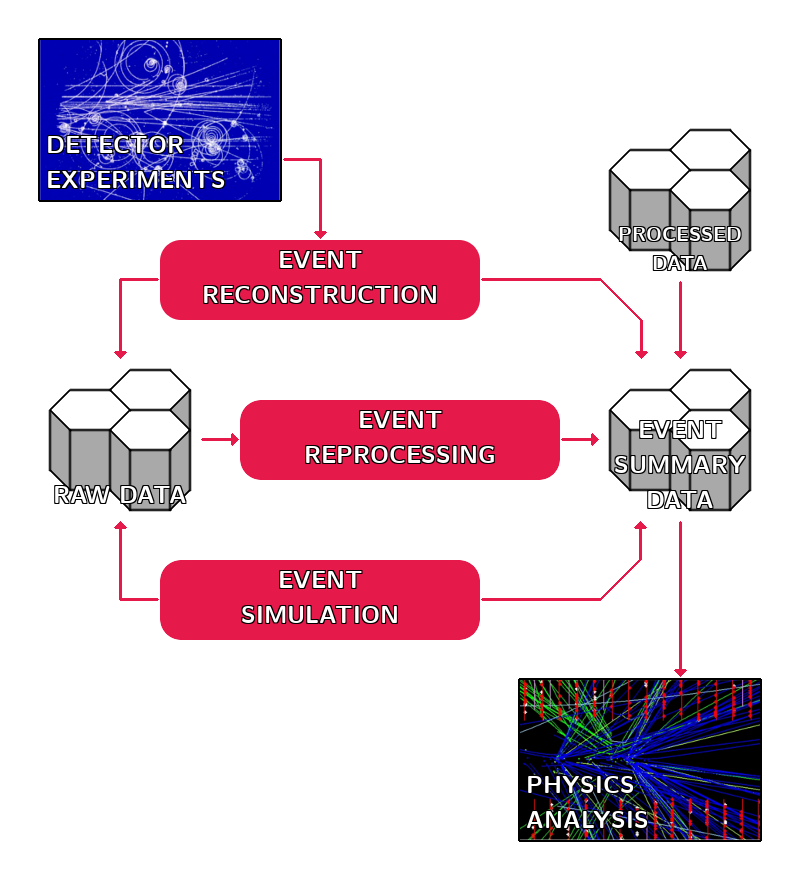
\includegraphics[scale=0.465]{data_processing}
        \caption{\label{fig:data_processing} Example data process found in particle detector software. Source: Own elaboration. Images used are freely available at \texttt{https://home.cern/}.}
    \end{figure}

% DONE UP UNTIL HERE!

A common problem that arises from this structure is the fact that, as technology progresses and particle detectors become more advanced, the produced data becomes more detailed and thus more expensive to process.
This issue is seen too at the Thomas Jefferson National Accelerator Facility (TJNAF) in Virginia, USA, where the linear accelerator and its paired detectors produce large amounts of data faster than what the available hardware can cope with. % Note: While this could use a citation, it only rises from conversations with Veronique and Vardan and afaik there ain't any formal documents regarding the issue.
Two natural solutions can be seen to this problem: Upscale the hardware to deal with the ever-increasing amounts of data to be processed; or improve the software to process more information without using new resources.
While the first option can't always be avoided, it's easy to see that the second is usually preferable since it helps alleviate the expenses of upgrading hardware.
In the present document, this second solution is explored by thoroughly going through each factor that slows down the data processing speed and assessing them separately.

% \newpage

% AREA IN COMPUTER SCIENCE/ENGINEERING
While the problem analyzed in this document belongs to the field of High Energy Physics, the effort done is more closely related to algorithms and complexity analysis.
This is attributed to the fact that the nature of the work lies in the underlying framework of the event reconstruction process, which in its core is about minimizing the error in a fit.
This by no means is a problem unique to physics.
Due to this, the contribution of this work has multiple objectives: It directly benefits the software development team at TJNAF in that it accelerates the software used, and it also provides a framework for other projects that look into speeding up the computation of the event reconstruction software for other particle accelerators or systems in general.

% A sample of these contributions would be, for example, the possibility of using mathematical tools for working with matrices such as the Sherman-Morrison formula, the matrix determinant lemma or the Cholesky decomposition for speeding up the update phase of an Extended Kalman Filter (EKF), described in Section \ref{ssec:prop_matrices}.

% The improvement in the processing time of the software brought by each step of the solution applied in this work can be seen in Figure \ref{fig:engines_times_improvements}.
% DCHB and DCTB are the engines used in the reconstruction software where this project's work is focused.

%     \begin{figure}[ht]
%         \centering
%         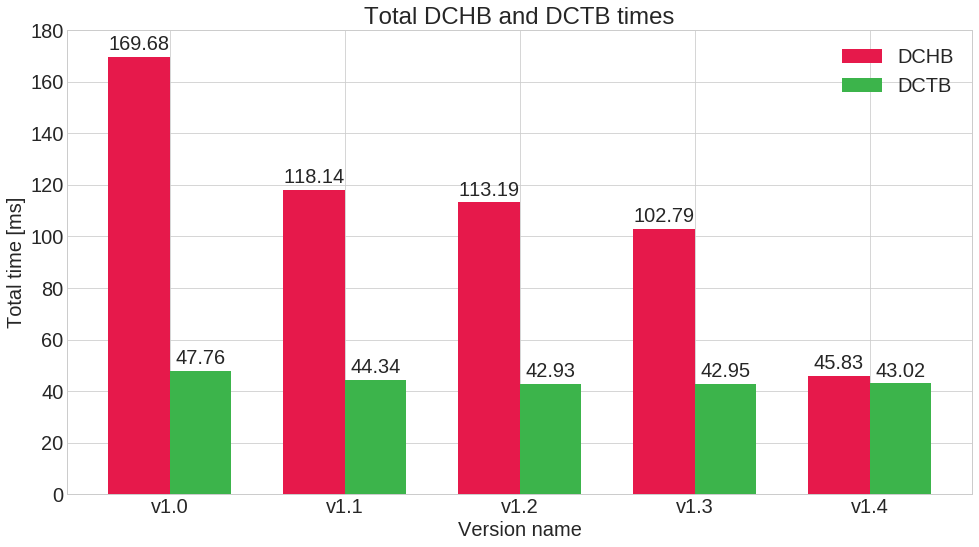
\includegraphics[scale=0.44]{engine_times/complete_improvement}
%         \caption{\label{fig:engines_times_improvements} Engine time improvements for DCHB and DCTB over the different versions. Source: own elaboration.}
%     \end{figure}

% \newpage

Figure \ref{fig:clas12_software_diagram} shows a detailed tree diagram of the CLAS12 software components.
CLAS12 is the reconstruction software used at TJNAF, and is described in detail in Section \ref{ssec:framework_clas12}.

    \begin{figure}[ht]
        \centering
        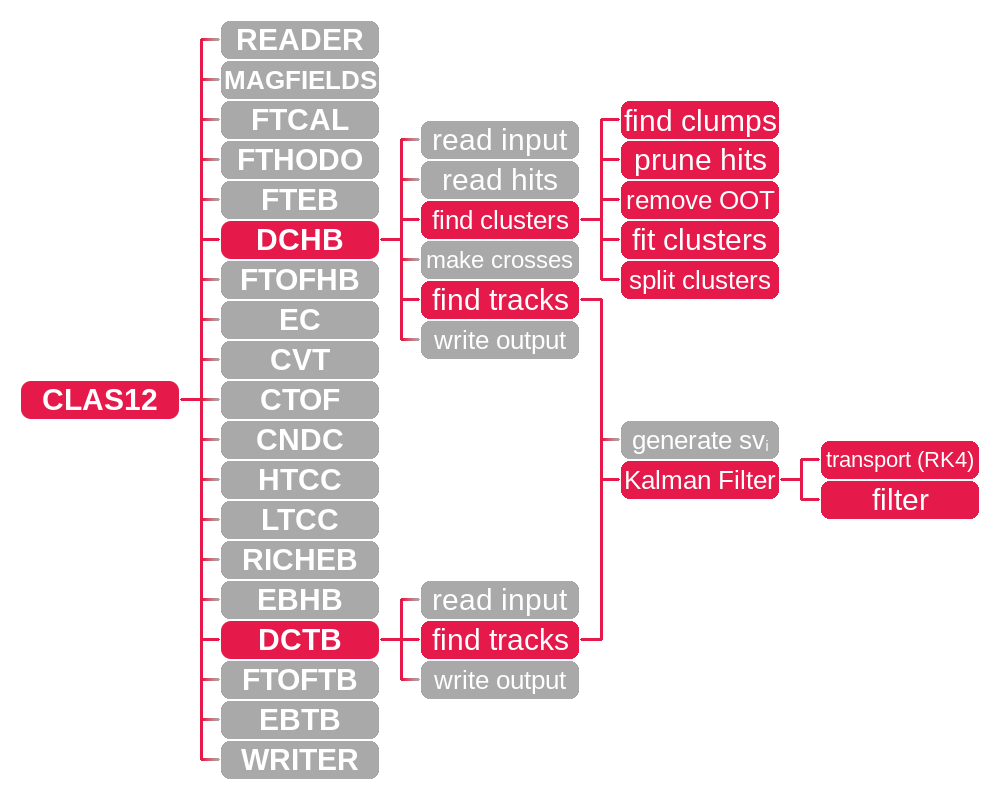
\includegraphics[scale=0.44]{clas12_software_diagram}
        \caption{\label{fig:clas12_software_diagram} Tree diagram with the CLAS12 software components. The components where the project's work is focused are highlighted.}
    \end{figure}

\newpage

Chapter $1$ presents a part of the current state of the art, along with a short description of each publication listed.
In Chapter $2$ the problem is formally defined, along with its context and the goals of the project.
In Chapter $3$ most of the large concepts that are related to the project and the document are explained, including the hardware and the software components.
Chapter $4$ elucidates in detail the profiling process described previously and presents the results of the profiling sessions.
Chapter $5$ explains the solutions implemented to each different bottleneck found in Chapter $4$ and proposes an algorithm for future work.
Then in Chapter $6$ the validity of the results produced after each change is asseverated and the computing times are compared.
Finally, Chapter $7$ provides with the concluding remarks of the work, including the setbacks faced and future work is proposed. % CHAPTER REFERENCE
    \newpage
    \secnumbersection{STATE OF THE ART} \label{sec:state_of_the_art}
A list of state-of-the-art methods aiming at similar objectives as the one described in this work follows:

\textbf{GPGPU Tracking in the COMET Phase-I Cylindrical Drift Chamber}~\cite{yeo2019gpgpu}: The COMET Phase-I experiment is a project in Japan that is aiming at discovering neutrinoless coherent transition of a muon to an electron in the field of an aluminum nucleus.
Just as in CLAS12, a Kalman filtering method is implemented to find the particle tracks, whose seeds are obtained by iterating through different combinations of hits using a fourth order Runge Kutta algorithm.
A seed is initial state vector that is fed to the filter, as is described in Section \ref{ssec:framework_ekf}.

This algorithm is implemented with the objective of finding the seeds with the minimum possible Distance Of Closest Approach (DOCA) to the wires in the detector, assigning only the seeds with a DOCA below a specific threshold to be investigated further with the Kalman Filter.
Due to the fact that the algorithm iterates through many combinations of seeds and that the operations that need to be done on them are constant, it is implemented as a parallel algorithm for a General Purpose Graphical Processing Unit (GPGPU).

This work is useful for the study of the event reconstruction software related to Drift Chambers (DC) because it shows that a commonly used algorithm for DC can be leveraged to a GPU, potentially reducing the computing times.

\textbf{Discriminative Training of Kalman Filters}~\cite{abbeel2005discriminative}: While useful in a plethora of fields, it's undeniable that the Kalman Filter is an essential tool in robotics due to its fine precision for state-estimation problems. % Note: I could add a citation here but a good reference is literally the same one I used for the title.
Considering this, scientists and engineers from the Department of Computer Science at the Stanford University brought up the idea of using machine learning algorithms to fine-tune the parameters in the filter and minimize the effect of perturbations or noise in the estimation of state vectors.

In view of this objective, various training algorithms with different objective functions in mind were developed, such as maximizing the joint likelihood of all the data, maximizing the measurement likelihood or the prediction likelihood, among others.
The way in which these algorithms help is in the fact that their output can help adjust the covariances of the EKF, in a way such that maximizes their predictive accuracy.

\textbf{Accelerating the Kalman Filter on a GPU}~\cite{huang2011accelerating}: As is described in Section \ref{ssec:prob_the_problem}, the usual cause for high computing times for the EKF are related to the matrix operations performed by the filter.
To counter this, the matrix computations can be leveraged to a GPU in order to accelerate the general computing time of the filter.

\cite{huang2011accelerating} implemented this approach and proved that the Kalman filter time on CPU is approximately linear with the state dimension while on GPU it can be sublinear due to its ease for computing matrix inversions and multiplications.
It's worth noting that while this publication is essential to most projects aiming to accelerate the KF, in the specific case of the CLAS12 software is not appropiate for because of the small size of the state vector being used~\cite{moravanszky2003dense}.

\textbf{GPU Enhancement of the Trigger to Extend Physics Reach at the LHC}~\cite{halyo2013gpu}: The idea of using computer vision and pattern recognition on detector data is explored by scientists at CERN, and considering that problems in this field were the origin of the GPU technology~\cite{pharr2005gpu}, they propose the idea of using these methods on detector data.

The main idea proposed in the publication is that of using the Hough Transform (described in Appendix \ref{add:hough_transform}) on a list of hits to find clusters following straight or curved lines.
Although this publication makes good use of the Hough Transform, it does not provide a framework for using it, it rather is proposed as a complement to the conventional combinational track finder algorithms commonly used in High Energy Physics.

\textbf{Kalman-Filter-Based Particle Tracking on Parallel Architectures at Hadron Colliders}~\cite{cerati2016kalman}: While not directly looking to reduce the total computing time of the particle tracking algorithm, this publication looks into parallelizing the algorithms used at the Large Hadron Collider (LHC) to make use of lower-power, multi-core processor units such as GPGPUs.

These improvements begin with the implementation of a custom matrix library named \textbf{Matriplex} which is optimized for dealing with small matrices (no larger than $6\,\times\,6$), like the ones used for particle tracking at the LHC.
To optimize the loading a small matrices into a GPU's memory, the library supports special vector registers for loading sets of matrices at once.
\textbf{Matriplex} also includes a code generator for generation of optimized matrix operations supporting symmetric matrices and on-the-fly matrix transposition.

To optimize memory management, \cite{cerati2016kalman} also try offloading the memory management work to a worker process or to another thread, thus grouping all memory operations together and removing redundant operations.

Continuing on the work with memory management, the size of the data structures used on the algorithm are also optimized in size to fit into the fastest cache memory.
This is done by replacing the hit data, the track data and the covariance matrices from object-oriented data structures to C-style arrays, along with the optimization of the contents of the data structures.
    \newpage
    \secnumbersection{PROBLEM DEFINITION} \label{sec:prob}
% ==- CONTEXT -=============================================
\subsection{Context} \label{ssec:prob_context}
% GENERAL DEFINITION OF A PARTICLE ACCELERATOR
A particle accelerator is a machine that can accelerate charged particles to very high speeds and contains them in well-defined beams via an electromagnetic field, providing an environment in which controlled collisions can occur so that particle physicists can study the small particles that result from these impacts~\cite{leduff2005longitudinal}.
It is important to note that due to the fact that the special theory of relativity requires that matter always travels slower than the speed of light in a vacuum, a particle will never reach this speed.
Due to this, the particle's speed is not thought of in traditional terms, but rather in terms of its energy or momentum, usually measured in electron Volts (eV).

As of the time of writing of this work, two types of accelerators are mainly used to study particle physics: the circular or cyclic radiofrequency (RF) and the linear accelerators.
The former is, as the name suggests, a ring, where the particles' track is bent into a circle, allowing them to re-use the same track as much as possible so that they can reach energies up to the order of Tera eV (TeV) in some cases, like the well-known Large Hadron Collider (LHC), at CERN~\cite{leduff2005longitudinal}.
The latter, usually denominated linear particle accelerators (linacs), accelerate particles by attracting them onto charged plates and switching their charge after the particles pass the plate to repel them, pushing them to the next plate.
While the particles accelerated by linacs generally achieve lower momenta than the ones pushed by their circular counterparts, they offer the advantage that they can produce a continuous stream of particles, whereas a cyclic accelerator can only periodically raise the particles to sufficient energy to merit a ``shot'' at the target~\cite{pinchoff2005introduction}.

% BRIEF DESCRIPTION OF JLAB, CEBAF AND CLAS12 (DETECTOR)
At the laboratory for which this work is done, TJNAF or Jefferson Laboratories (JLab) research is assisted by the use of one such linac, the Continuous Electron Beam Accelerator Facility (CEBAF).
CEBAF is composed of a polarized electron source and a pair of superconducting radiofrequency linear accelerators connected to each other by two arc sections that contain steering magnets~\cite{leemann2001continuous}.
The peculiar design of CEBAF allows for the continuous beam characteristic of other linacs, while also being able to reuse the tracks, effectively reaching energies found in an accelerator ten times its size~\cite{leemann2001continuous}.
A picture of CEBAF can be seen in \ref{fig:cebaf}.

    \begin{figure}[ht]
        \centering
        \fbox{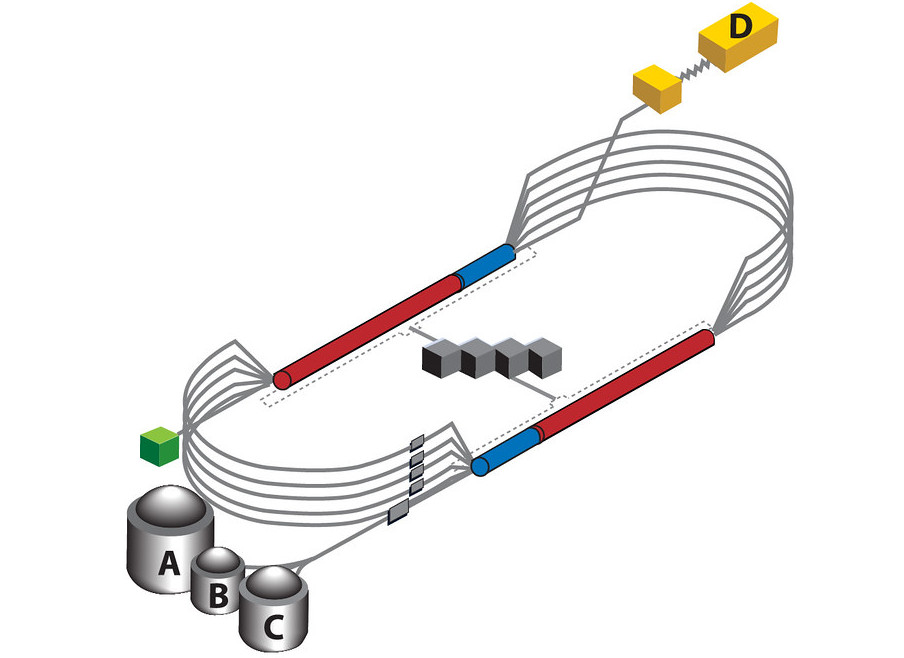
\includegraphics[scale=0.36]{cebaf}}
        \caption{\label{fig:cebaf} The Continuous Electron Beam Accelerator Facility (CEBAF). Source: \texttt{https://www.flickr.com/photos/jeffersonlab/12599705145}}
    \end{figure}

The produced beam ends at one of the four available experimental halls, labeled Hall A, B, C and D, each containing specialized spectrometers to record the products of collisions between the electron beam with itself or with a stationary target.
Particularly, in experimental Hall B, the detector utilized to study the results of these collisions is the CEBAF Large Accelerator Spectrometer for 12 GeV (CLAS12), where each particle-target collision, commonly denominated ``event'', is captured.
This is done in an order of up to several thousand events per second, and the recorded data is later transferred to a farm of computing processors for teams of physicists to analyze them and look for new kinds of particles or information related to the structure of different particles~\cite{mecking2003cebaf}.

% BRIEF DESCRIPTION OF AN EVENT RECONSTRUCTION SOFTWARE
Most particle detectors deal with enormous amounts of data, usually too large to be analyzed ``by hand'' by the physicists trying to understand it, so it's common to build software that aids in the analysis process by filtering the useful data from the background noise~\cite{demchenko2013addressing}.
In the case of CLAS12, this software follows a Service Oriented Architecture (SOA) and consists of the framework, event reconstruction, visualization, calibration, monitoring services as well as detector and event simulator.
The scope of this work is centered mostly with the framework and the event reconstruction software, which are the CLAs12 Reconstruction and Analysis framework (CLARA) and the event reconstruction software itself, specifically with its components associated to the Drift Chambers (DC).

Roughly speaking, the CLARA framework acts as a fairly simple to use system to separate different sections of the software into services which run in so-called Data Processing Environments (DPEs).
The DPEs allow for easy scaling of the software by leaving the distribution of the hardware resources to CLARA~\cite{gyurjyan2013clara,gyurjyan2015component} using the ZeroMQ message transfer protocol~\cite{hintjens2013zeromq}.
The event reconstruction software works by analyzing the data obtained from each of the different components of the CLAS12 detector and tries to reconstruct the event, as its name suggests~\cite{ziegler2013clas12}.

% BRIEF DESCRIPTION OF THE DRIFT CHAMBERS AND THEIR SOFTWARE IMPLEMENTATION
Like any particle detector, CLAS12 is divided into a series of many different components that detect different types of particles utilizing a variety of detection methods~\cite{pinchoff2005introduction}.
One such kind of detectors are the Drift Chambers (DC), which work by measuring the fluctuations in the charge of the matter inside the chambers and in turn try to ``guess'' what passing particle caused such difference in charge.
This measurement is obtained via a set of wires acting as cathodes which, in the case of CLAS12, are strung inside 18 wire chambers inside 3 hexagonal shapes, each with 2 superlayers of 6 layers with 112 wires each, thus having a total of 24,192 wires~\cite{mestayer2017clas}.
These measurements are obtained with the hope that a set or cluster of hits in different wires will allow to estimate the trajectory of the particle that caused these hits and in turn understand its properties.
A diagram of the CLAS12 detector can be seen in Figure \ref{fig:dc_horizontal_cut}, where two particle trajectories are marked in a pointed line.
The wires hit by each trajectory are marked in red in the image to the left and the area that is detected by each wire is denoted by the hexagons in the image to the right.

    \begin{figure}[ht]
        \centering
        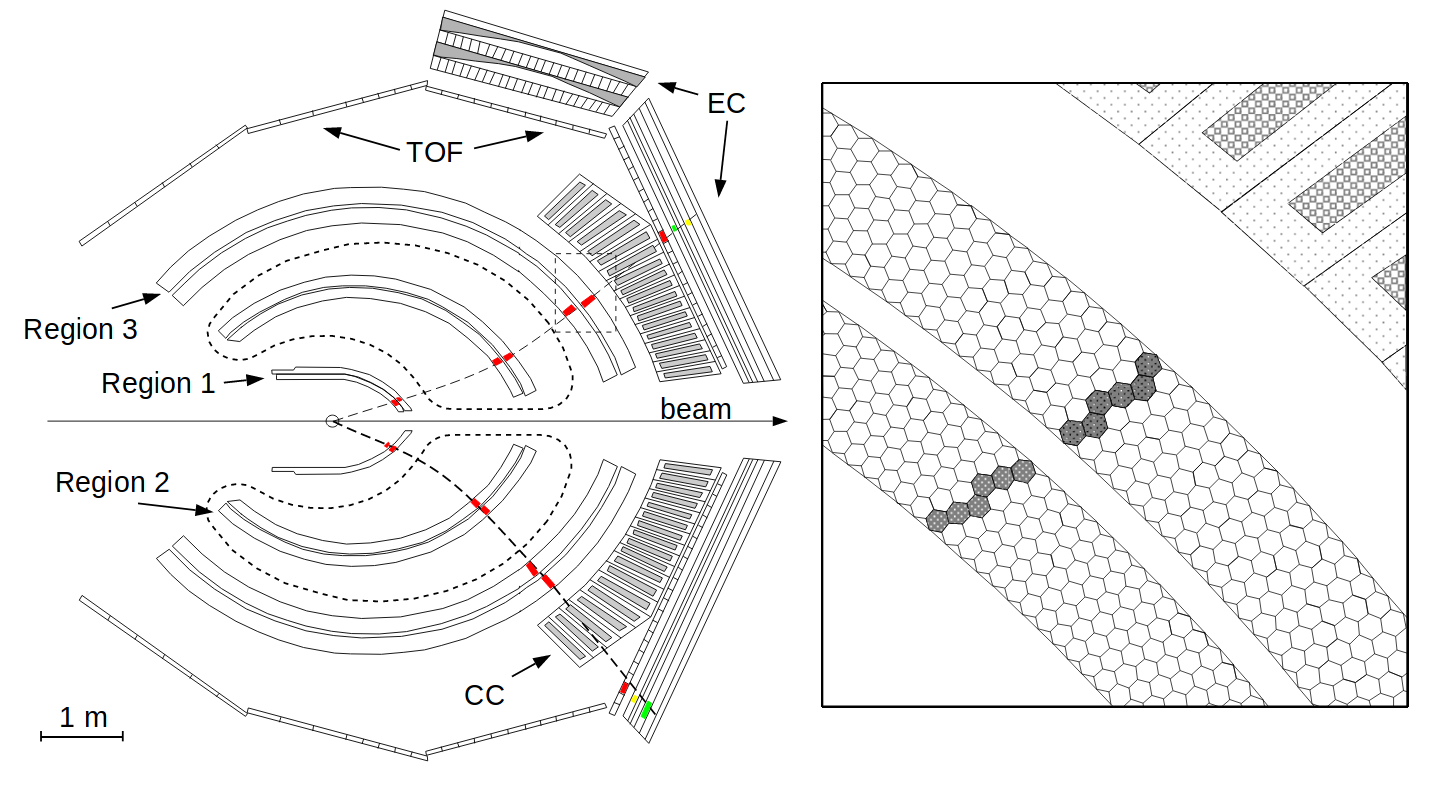
\includegraphics[scale=0.30]{dc/horizontal_cut}
        \caption{\label{fig:dc_horizontal_cut} Horizontal cut through the CLAS detector at beam line elevation showing two charged particles traversing the $18$ superlayers in the $3$ regions of the drift chambers in opposite sectors. The picture to the right shows an enlargement of the boxed area in the picture to the left. Source: The CLAS Drift Chamber System~\cite{mestayer2000clas}.}
    \end{figure}

% ==- THE PROBLEM -=========================================
\subsection{The Problem} \label{ssec:prob_the_problem}
% BRIEF DESCRIPTION OF PARTICLE TRACKING AND THE KALMAN FILTER
Different algorithms are used to estimate the trajectory or track of some of the particles that are ejected in each event, and these algorithms belong in a field named particle tracking.
In the specific case of the DC in CLAS12, particle tracking is done via the Extended Kalman Filter (EKF), which is a popular algorithm for estimating the position of a moving object with a good precision given that the path followed by it can be modeled by deterministic movement equations and that measurements (i.e: the ones taken by the wires) can be obtained for this object's position over time.
This makes it a good estimator for the charged particles ejected by the target after each event~\cite{kalman1960new}.

The EKF shows great performance at its task in the reconstruction software, but it suffers from the disadvantage that it is a fairly slow algorithm.
To reach the previously mentioned precision, both the Kalman Filter (KF) and its extended counterpart require matrix multiplications and inversions when computing states, as well as the calculation of Jacobian matrices, as is described in Section \ref{ssec:framework_ekf}.
These matrix operations mean that the computational complexity of the algorithm is quite high, which in big-O notation is:
    \begin{equation*}
        O(\text{C}(\mathbf{f}(\cdot, \cdot)) + \text{C}(\mathbf{h}(\cdot)) + n^3 + n^2\,m + n\,m^2)\,,
    \end{equation*}

% \newpage

where $n$ and $m$ are the state and measurement vector sizes and $C(\mathbf{f}(\cdot, \cdot))$ along with $C(\mathbf{h}(\cdot))$ are used to denote the costs of $\mathbf{f}(\cdot, \cdot)$ and $\mathbf{h}(\cdot)$ respectively, where $\mathbf{f}$ and $\mathbf{h}$ are the transition functions between two arbitrary timesteps $k$ and $k+1$ for the state vector $\mathbf{x}_k$ and the measurement vector $\mathbf{z}_k$ respectively.
The mathematical formulation of the model and the calculation of the computational complexity of each operation are described in detail in Section \ref{ssec:framework_ekf}.

Something to note is that while most systems using the Kalman Filter are slowed down because they process large state and measurement vectors with large covariance matrices, the DC software suffers from a different issue.
The $n$ and $m$ mentioned before are constants $5$ and $6$ respectively, but the state transition itself between states $k$ and $k+1$ takes a large amount of time and is iterated over a large number of times as is described in Sections \ref{ssec:framework_ekf}, \ref{ssec:framework_tf} and \ref{ssec:framework_rk4}.
Even more, the Kalman Filter is used as a fixed point iteration to compute the state vector at the last measurement site $K$ with enough precision, requiring many runs to obtain precise results.

This large computation time takes a heavy toll on the total running time of the two engines that process the DC data in the reconstruction software: the DC Hit-Based tracking engine (DCHB) and the DC Time-Based tracking engine (DCTB); taking a total of $49.3\%$ of the total running time of the whole CLAS12 software.
It's also worth noting that the second component in terms of processing time is the Cluster Finding used in DCHB and DCTB, which takes in total a $40.1\%$ of the previously mentioned time.
To better visualize the impact on the processing time of the DCHB and DCTB components, see Figure \ref{fig:engines-times-sep2018}.
As all the other performance tests in this document, these measurements were obtained by running the CLAS12 software on $10.000$ events with real experimental data.
The test file used is named \texttt{clas\_004013.0.hipo}, and can be obtained by contacting the Hall B team at Jefferson Lab (https://www.jlab.org/Hall-B/).

    \begin{figure}[ht] % Note: Maybe I could mention the github's HEAD used to obtain this?
        \centering
        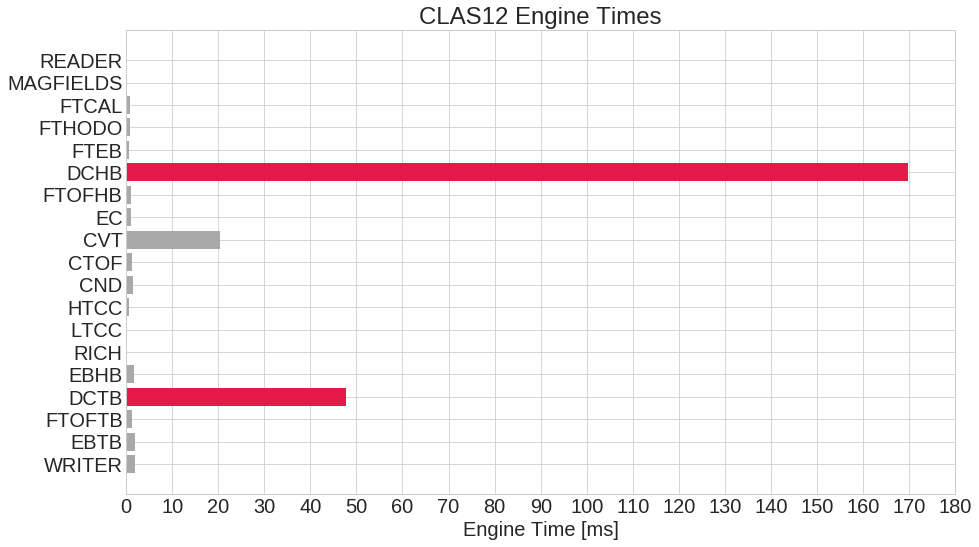
\includegraphics[scale=0.44]{engine_times/1_0}
        \caption{\label{fig:engines-times-sep2018} CLAS12 Engine times as of September 7th, 2018.}
    \end{figure}

The problem that this project focuses on is that of reducing the total computation time of the whole CLAS12 offline software.
To tackle the problem, the project focuses in the slowest components of CLAS12, DCHB and DCTB, and especifically to the acceleration of the Kalman Filter used in these two DC engines.
Another smaller part of the project also focuses in the acceleration of the cluster finding algorithm, considering that it is the second largest bottleneck in the software's execution.

% \newpage

% ==- GOALS -=============================================== %
\subsection{Goals} \label{ssec:prob_goals}
As can be seen in Figure \ref{fig:engines-times-sep2018}, the combined time taken by the DCHB and DCTB engines is as much as $86.35$\% of the total execution time of the CLAS12 software, making them prime candidates for accelerating the reconstruction software.
Therefore, the main goal of this project is to reduce the total running time of the CLAS12 software by specifically accelerating the KF algorithm currently implemented in the code while also trying to tackle the cluster finding algorithm to a lesser extent.
The project's major goals are:

\newpage

    \begin{itemize}
        \item Compare a set of the different Java profilers and analyze which one is the most useful to measure the CLAS12 software performance.
        \item Study which components of the KF and Cluster Finding algorithms implemented in CLAS12 can be accelerated via optimizations and/or parallelization.
        \item Study the way in which these optimizations and/or parallelizations could take place in the context of execution of the software, the CLARA framework.
        \item Effectively apply the optimizations and implement the algorithms that would allow a substantial improvement in the running time of the software.
        \item Profile and test the code continuously while applying changes, ensuring that the output data is consistently the same through the development process.
        \item Document the changes made to the code and describe in detail the algorithms and optimizations implemented in order to help future related work.
    \end{itemize}

It's worth noting that these objectives differ slightly from the ones originally proposed for this project: Originally only parallelization techniques were going to be tested, but during development it was decided to apply general optimizations.
    \newpage
    \secnumbersection{CONCEPTUAL FRAMEWORK} \label{sec:framework}
\subsection{The CLARA Framework} \label{ssec:framework_clara}
CLARA is a SOA platform designed to build streaming scientific-data analytics applications that allows users to process data as streams across data centers and clouds~\cite{gyurjyan2011clara}.
The framework is used both in JLab for CLAS12 and in NASA for the NASA Information and Data System (NAIADS) and Surface Radiation Budget (SRB) projects~\cite{lukashin2015earth}.

As defined in the Introduction, a data event is the collision of a beam of particles into a target which results in a shower of particles.
A data processing engine or simply engine is a software component that processes the data event, usually reconstructing the data obtained in a specific detector component or providing a secondary functionality.

The CLARA framework consists of four core components: A Data Processing Station, a Pipe, a Data Processing Environment and an Orchestrator:
    \begin{itemize}
        \item \textbf{Data Processing Station}: Usually referred to as a CLARA station, the Data Processing Station acts as a container for a user-made data processing engine.
        In the context of the CLAS12 software, this acts as the container for each engine associated to a hardware component of the CLAS12 detector, with a simple relationship of one station for one engine.
        This station-engine coupling is denoted as a Data Processing Service or simply service, and can be seen in Figure \ref{fig:clara_service}.
        
            \begin{figure}[ht]
                \centering
                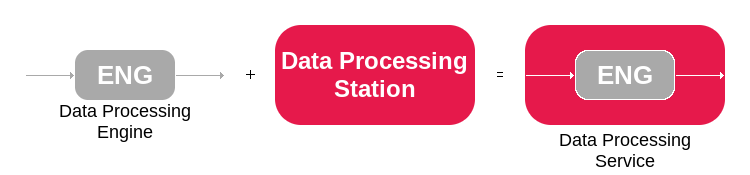
\includegraphics[scale=0.50]{clara/service}
                \caption{\label{fig:clara_service} Data engine and CLARA station coupling.}
            \end{figure}
        
        \item \textbf{Data Stream Pipe}: A data bus based on the xMsg messaging system, which in turn is based on the ZeroMQ protocol~\cite{hintjens2013zeromq}.
        xMsg is a messaging protocol based on the publisher-subscriber pattern which allows for various agents to communicate based on topic subscriptions.
        In the context of the CLAS12 software, the data buses act as pipes between services, allowing one service to send Data Events to another.
        The interaction between stations and pipes can be seen in Figure \ref{fig:clara_station_pipe}.
        
            \begin{figure}[ht]
                \centering
                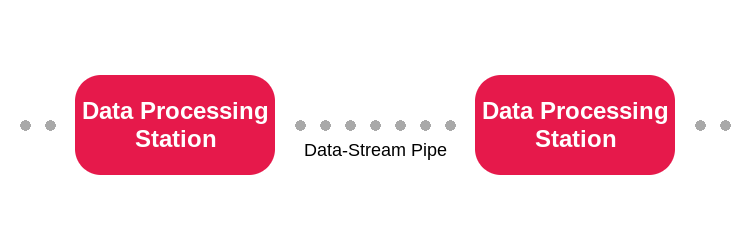
\includegraphics[scale=0.50]{clara/stations_and_pipes}
                \caption{\label{fig:clara_station_pipe} CLARA stations coupled with pipes.}
            \end{figure}
    
        \item \textbf{Data Processing Environment (DPE)}: A DPE is a container unit for one or more services and their corresponding data pipes which acts as a communications hub between the services and the hardware.
        Communication between DPEs can be done using the same data stream pipes.
        Different DPEs can be placed in different computing environments, thus allowing the communication of different services between different machines.
    
        \item \textbf{Data Flow Orchestrator}: The Orchestrator is a system to coordinate the communication between the Data Processing Services via the Data-stream Pipes.
        In CLAS12, the Orchestrator simply forms a straight line between services which is called ``Production Chain'', and each service alters the Data Event as it sees fit to then have the engines following read and write it.
        To setup a production chain such as the one seen in Figure \ref{fig:clara_production_chain}, the Orchestrator must be used to configure each service and pipe to allow the free flow of data.
        
            \begin{figure}[ht]
                \centering
                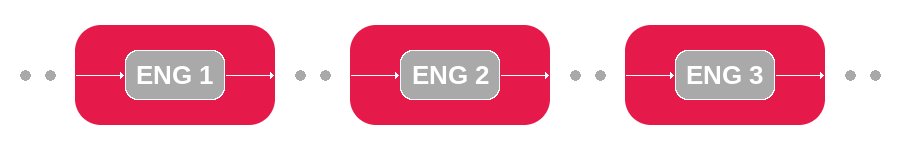
\includegraphics[scale=0.50]{clara/production_chain}
                \caption{\label{fig:clara_production_chain} CLARA production chain.}
            \end{figure}
            
    \end{itemize}
\newpage
\subsection{CLAS12 Offline Software} \label{ssec:framework_clas12}

The CLAS12 Offline Software is the software associated to reconstructing the data detected at the CLAS12 detector from Hall B.
It is separated into two components: \textbf{common tools} and \textbf{reconstruction}~\cite{ziegler2013clas12}.

The \textbf{common tools} package is a set of libraries developed by the physicists at JLab that contain all the tools that are commonly reused by different engines, like the \textbf{detector geometry} or \textbf{magnetic fields} packages.
The \textbf{reconstruction} package, which is where most of this work is focused, is composed by a set of semi-independent engines connected via the aforementioned CLARA pipes, where each detector component is represented by one or more CLARA Data Processing Services.

These services are separated into two categories, ones that ``help'' the data flow (Event Builders, IO, etc) and others that describe the hardware of the CLAS12 detector.
A diagram of the detector can be seen in Figure \ref{fig:clas12_hardware_design}.

    \begin{figure}[h]
        \centering
        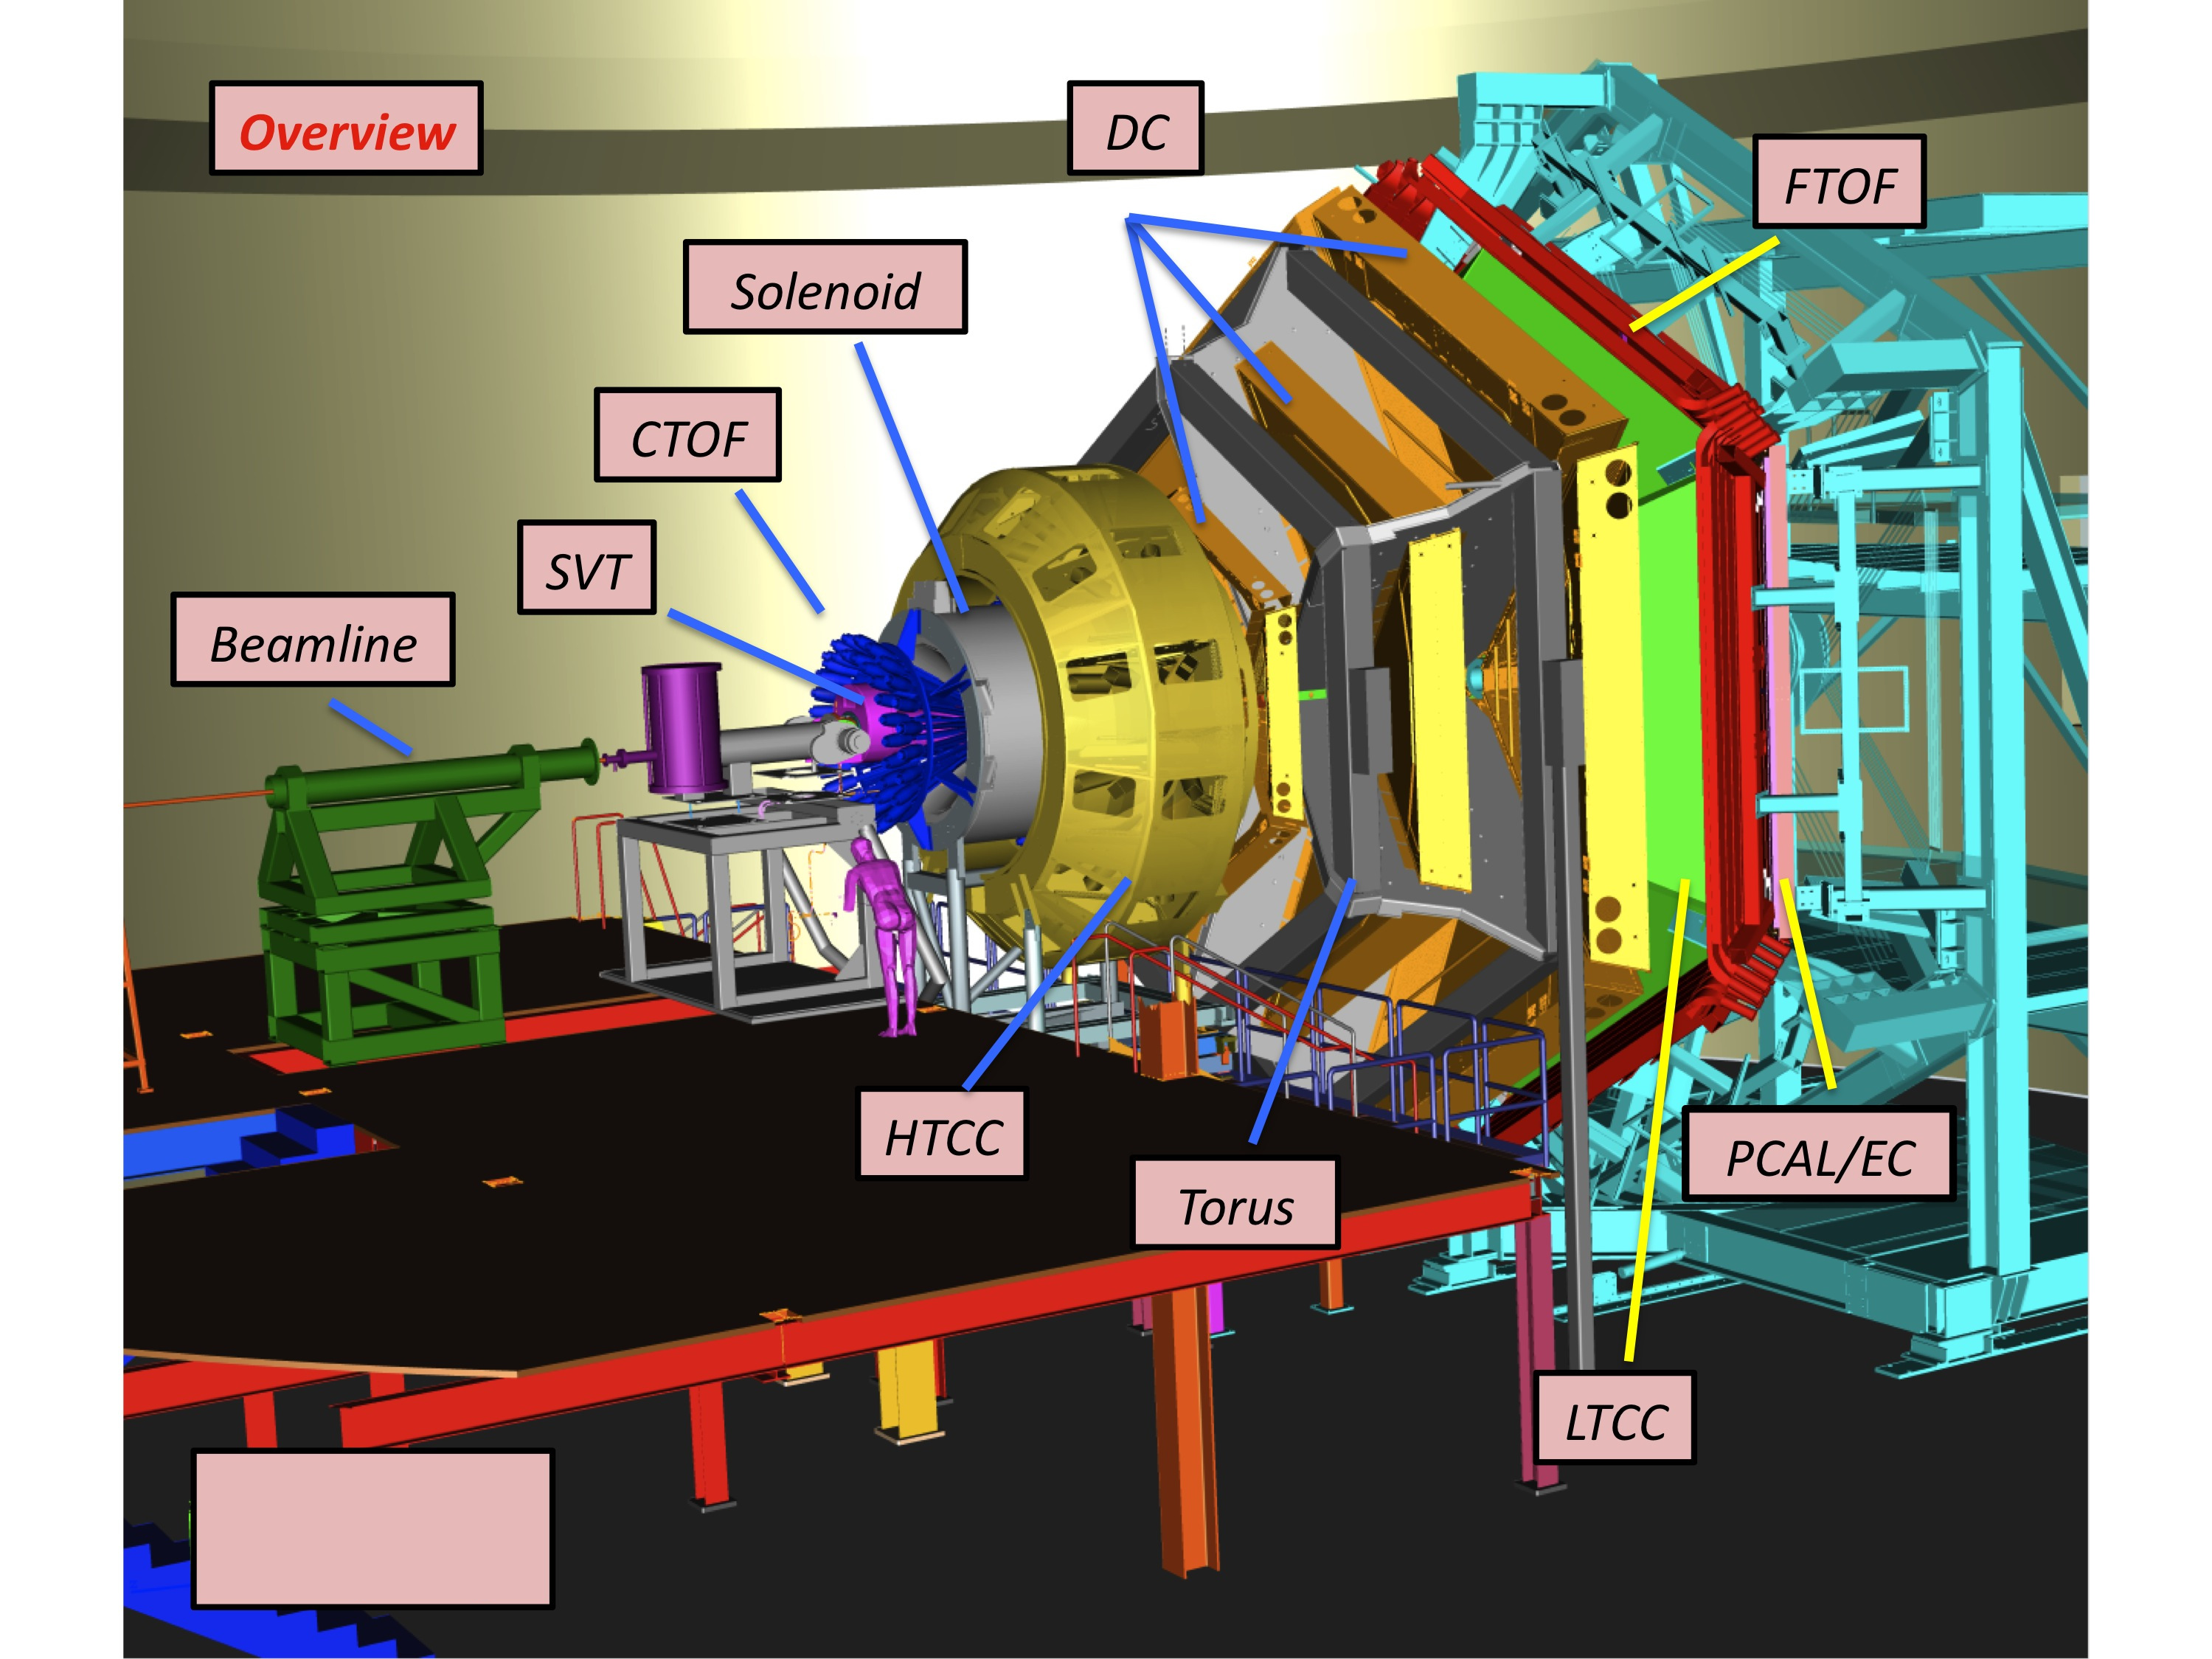
\includegraphics[scale=0.147]{clas12_hardware_design}
        \caption{\label{fig:clas12_hardware_design} CLAS12 detector hardware design. Source: CLAS12 web (\texttt{https://www.jlab.org/Hall-B/clas12-web/}).}
    \end{figure}

\newpage

A comprehensive list of CLAS12 software engines and their associated physical components (when available) is given.
It is worth noting that many engines run twice for each data event, first running a Hit-Based (HB) analysis and then a Time-Based (TB) analysis.
HB analysis is done without using time-related data and is mainly used to filter through the data and eliminate noise, while TB analyzes the filtered data and finds the final particle tracks.
    \begin{itemize}
        \item \textbf{HIPO READER and WRITER}: Engines that provide the file reading and writing, based on the HIgh Performance Output (HIPO) data format~\cite{gavalian2019data}. % Note: I could describe HIPO further, but it doesn't come in anytime during the whole thesis so idk.
        
        \item \textbf{Event Builder Hit-Based (EBHB) and Event Builder Time-Based (EBTB)}: Engines that build the data events from the HIPO data and pass them to the other engines.
        
        \item \textbf{MAGFIELDS}: Engine providing a model for the magnetic field inside the detector, used by components that need to estimate a particle's trajectory. % Note: I could describe how the magnetic field is simulated, but idk if it's really necessary.
        
        \item \textbf{High Threshold Cherenkov Counter (HTCC) and Low Threshold Cherenkov Counter (LTCC)}: Engines detecting particles moving faster than the local speed of light in a medium utilizing the emitted cone of light.
        The HTCC detects pions with high momenta ($>5~GeV/c$), while the LTCC the ones with low momenta ($>3~GeV/c$), and both are part of the Forward Detector (FD), a superconducting Torus magnet that covers the range from $5\degree$ to $40\degree$ measured from the source of the event, as can be seen in Figure \ref{fig:dc_horizontal_cut} from Section \ref{ssec:prob_context}.
        
        \item \textbf{DC Hit-Based tracking (DCHB) and Time-Based tracking (DCTB)}: The engines where most of the work in this thesis is focused, and are explained in detail in Section \ref{ssec:framework_dc}.
        Part of the FD.
        
        \item \textbf{Forward Time-Of-Flight Hit-Based detector (FTOFHB) and Time-Based detector (FTOFTB)}: Plastic scintillators that provide precise time-of-flight measurements for charged particle identification up to $4.5~GeV/c$.
        Scintillators are materials that show a scintillation or flash of light when excited by ionizing radiation.
        Part of the FD.
        
        \item \textbf{Ring Imaging Cherenkov (RICH) Detectors}: Similar in design to the FTOF detector, but capable of detecting charged particles with momenta of up to $8~GeV/c$ instead of $4.5$.
        Part of the FD.
        
        \item \textbf{Electromagnetic Calorimeter (EC)}: Allows for the detection of single high-energy photons by using a pre-shower calorimeter, improving spatial resolution and the separation of two photos for momenta of up to $10~GeV/c$.
        In particle physics, a shower refers to the cascade of secondary particles after the collision between the beam and the target.
        Part of the FD.
        
        \item \textbf{Central Time-Of Flight detector (CTOF)}: A scintillator array allowing for pion identification in a momentum range of up to $1.2~GeV/c$.
        Part of the Central Detector (CD), which is a superconducting Solenoid magnet that covers the polar angles from $35\degree$ to $135\degree$.
        
        \item \textbf{Central Neutron Detector (CND)}: A barrel with scintillator bars that detects high energy neutrons with an efficiency of up to $15\%$.
        The efficiency of a neutron detector refers to how many neutrons that pass through it are detected~\cite{pinchoff2005introduction}.
        Part of the DC.
        
        \item \textbf{Forward Tagger (FT) electromagnetic calorimeter (FTCAL), FT tracker (FTEB) and FT scintillation counter (FTHODO)}: An extension of the CLAS12 capabilities that allows it to detect electrons and photons at angles as low as $2.5\degree$.
        
        \item \textbf{Silicon Vertex Tracker (SVT) and Barrel Micromegas Tracker (BMT)}: Reconstruct the trajectories of charged tracks in the angular region from $35\degree$ to $125\degree$ with a momenta up to $1~GeV/c$.
        In the code, both components are contained inside the CVT engine.
    \end{itemize}

The production chain integrating all of the engines that represent these detectors can be seen in Figure \ref{fig:engines-chain}.

    \begin{figure}[h]
        \centering
        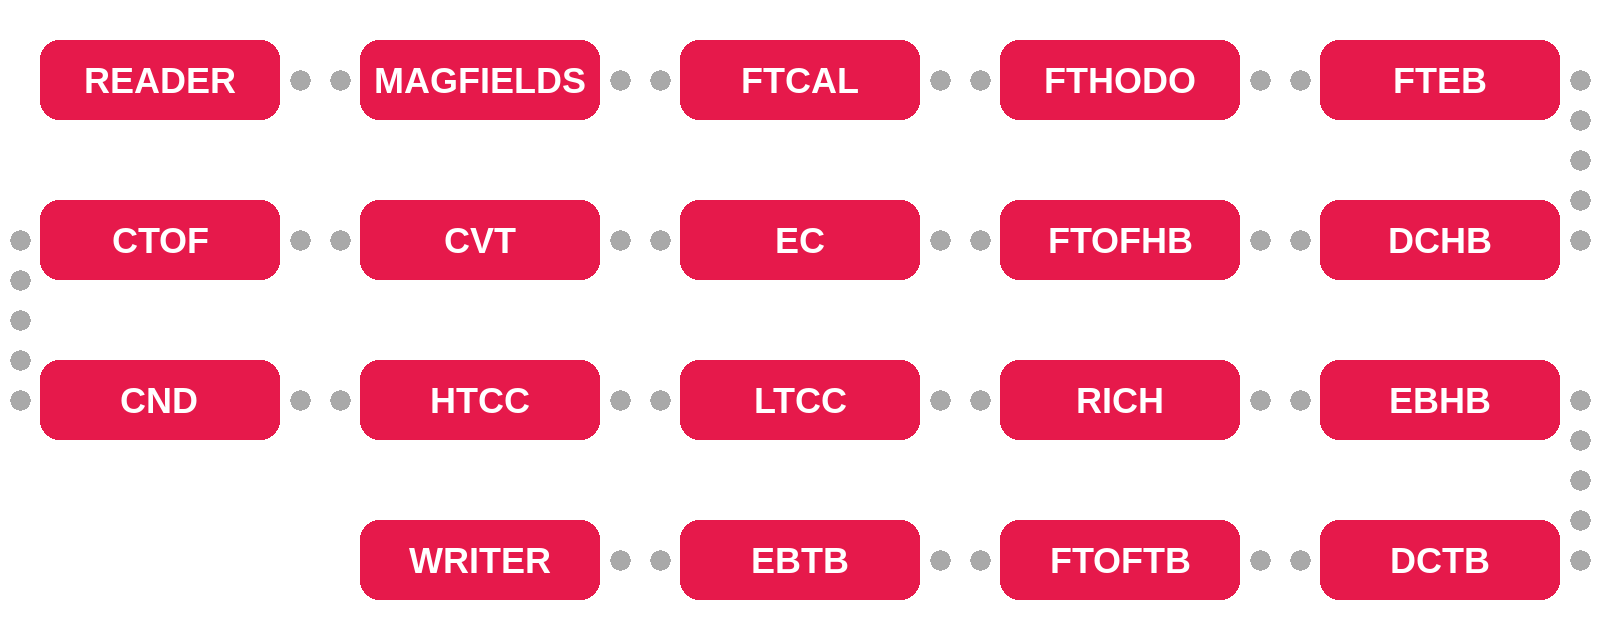
\includegraphics[scale=0.27]{engines_chain.png}
        \caption{\label{fig:engines-chain} CLAS12 engines production chain.}
    \end{figure}
    
\newpage
\newpage
\subsection{Drift Chambers} \label{ssec:framework_dc}
Drift Chambers in general are a type of Multiwire Proportional Chambers (MPC) that use an array of wires at high voltage running through a chamber held at ground potential which is filled with gas.
Any ionized particle passing through the chamber will ionize its surrounding atoms, accelerating them across the chamber so that they can be collected by the nearest wire.
By computing the different pulses on each of these wires, the trajectory of the particle can then be estimated~\cite{sauli1977principles}.

DC differentiate themselves from MPC by the fact that they can obtain very precise measurements of the timing of the pulses from the wires along with the information commonly obtained by MPC.
This allows a more precise estimation of the distance at which the particle passed the wire and greatly improves the accuracy of the path reconstruction~\cite{blum2008particle}.

As can be seen in Figures \ref{fig:dc_horizontal_cut} and \ref{fig:dc_vertical_cut}, the CLAS12 Drift Chamber system measures the momentum of charged particles emerging from the target using a set of $18$ wire chambers distributed into $3$ regions with $6$ wire chambers each.
Each wire chamber consists of $2$ superlayers, while each superlayer of $6$ layers and each layer of $112$ wires, making up to a total of $24,192$ sense wires strung on the entire machine~\cite{mestayer2000clas}
    
    \begin{wrapfigure}{r}{0.51\textwidth}
        \centering
        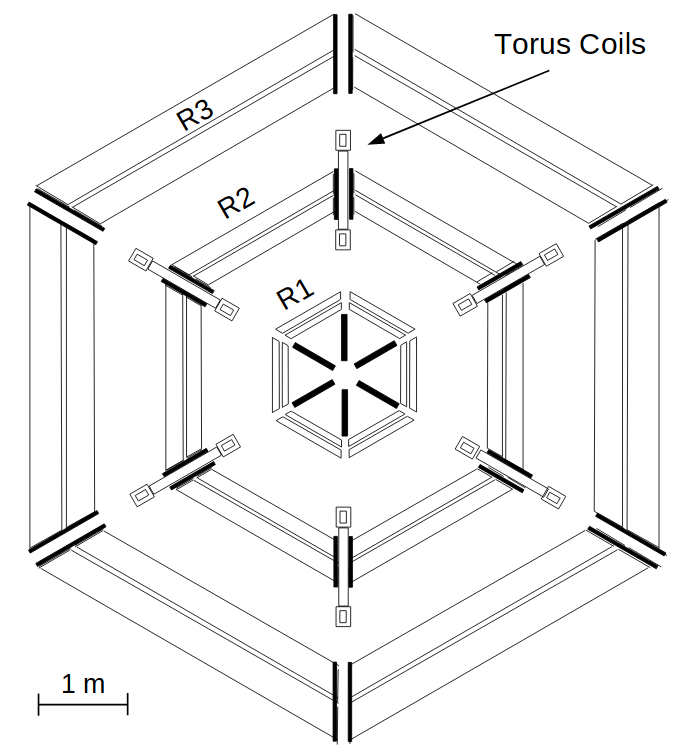
\includegraphics[width=1\textwidth]{dc/vertical_cut}
        \caption{\label{fig:dc_vertical_cut} Vertical cut through the drift chambers transverse to the beam line at the target location. Source: The CLAS Drift Chamber System~\cite{mestayer2000clas}.}
    \end{wrapfigure}

After obtaining the measurements, the DCHB and DCTB CLARA engines run to process them and deduce the tracks of the detected particles.
Pattern recognition for the DC is first done on a hit-based basis, where a hit is defined as a wire with a recorded signal.
Prior to searching for track segments (groups of hits) in each superlayer, a hit-pruning algorithm is employed to reject apparent noise, which is defined based on the number of contiguous hits in a layer.

Since the particles should go through layers close to horizontally, if many hits are detected contiguously in one layer it usually means that either the wires are malfunctioning or various wires are detecting the same particle, so unnecessary hits are rejected.

The pruned hits are then grouped into clusters, defining a cluster as a contiguous set of hits spanning through different layers in a superlayer.
A more detailed description of the cluster finding algorithm is given in Section \ref{ssec:framework_cf}.
The pairs of clusters in two adjacent superlayers are denoted as crosses.
Linear fits to these crosses serve as cluster refiners and are a preliminary step to estimating a particle's trajectory or track.

Then, a fit is done to sets of three crosses which can be linear o curved depending on the strength of the local effect of the magnetic field in the particle's trajectory.
This fit is commonly denoted as track fitting.
Track parameters are estimated in the global coordinate system of the detector from this trajectory, and are then fed as input to the Kalman Filter, which refines an estimate of the parameters of a track.

A general description of the KF algorithm is explained in Section \ref{ssec:framework_ekf}, while the specific implementation done for the track finding in CLAS12 can be read in Section \ref{ssec:framework_tf}.
\newpage
\subsection{Cluster Finding} \label{ssec:framework_cf}
    \begin{wrapfigure}{r}{0.51\textwidth}
        \centering
        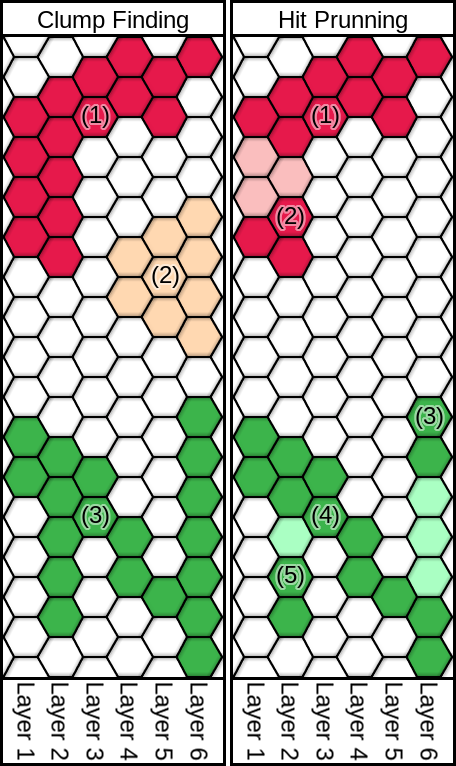
\includegraphics[width=1\textwidth]{clus_finding/00_01}
        \caption{\label{fig:cf_figure1} Clump Finding \& Hit Pruning algorithms over the layers in a superlayer.}
    \end{wrapfigure}

The Cluster Fitting algorithm used at the DC can be described by dividing it into the five algorithms that conform it, which are \textbf{Clump Finding}, \textbf{Hit Pruning}, \textbf{Out of Timers Removal}, \textbf{Cluster Fitting} and \textbf{Cluster Splitting}.

\textbf{Clump Finding}: A clump is defined as a simple set of adjacent hits that spans at least \texttt{DC\_MIN\_NLAYERS} layers, which is a constant at CLAS12 usually set at $4$.
In the image to the left of Figure \ref{fig:cf_figure1}, the clusters formed from a group of hits in one superlayer is denoted.
Each clump formed from the hits is marked using a different color and is also denoted using a simple numbering system.
Running the clump finding algorithm on this group of hits, it can be seen that clumps ($1$) and ($3$) are valid since they span at least $4$ layers while clump ($2$) is invalid for the opposite reason.

\textbf{Hit Pruning}: Hits that are considered noise are pruned in this step.
Four cases are considered for each sequence of hits in a layer: \textbf{(I)} if the sequence contains more than $10$ hits, all hits are considered noise and are removed.
\textbf{(II)} If the sequence contains between $5$ and $10$ hits, only two at each end of the sequence are conserved.
\textbf{(III)} If the sequence contains between $2$ and $4$ hits, only one hit from each end is conserved.
\textbf{(IV)} If $2$ or less hits are in the sequence, no hits are removed.

In the image to the right of Figure \ref{fig:cf_figure1}, the hits removed from each clump are denoted by a lighter color than the ones that stay.
After running the pruning algorithm, the \textbf{Clump Finding} algorithm is ran again on the now pruned hits.
The new clumps are denoted again in the image, with clumps ($2$), ($3$) and ($5$) considered invalid.

\newpage

    \begin{wrapfigure}{l}{0.49\textwidth}
        \centering
        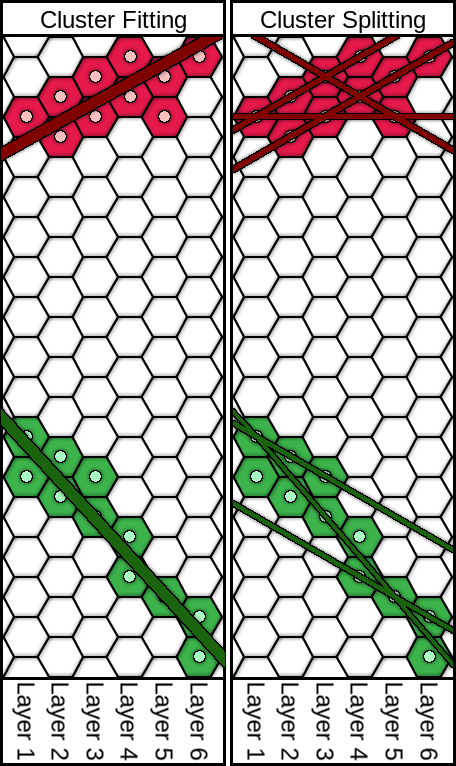
\includegraphics[width=1\textwidth]{clus_finding/02_03}
        \caption{\label{fig:cf_figure2} Cluster Fitting and Splitting algorithms over the layers in a superlayer.}
    \end{wrapfigure}

\textbf{Out of Timers (OOT) Removal}: This method iterates through all the hits in each clump and removes the ones considered Out of Timers.

``Out of Timers'' are hits that have a Distance Of Closest Approach (DOCA) higher than their cell size.
A hit's DOCA refers to the closest distance between the charged particle and the center of the wire in the particle's trajectory, and is measured by analyzing the fluctuations in the wire's charge through time~\cite{blum2008particle}.
A wire's cell size simply refers to the size of the side of the hexagonal cell that contains the wire, as can be seen in Figures \ref{fig:cf_figure1} and \ref{fig:cf_figure2}.

\textbf{Cluster Fitting}: After the clumps are pruned and cleaned from out of timers, a linear fit is attempted for each.
The fit is considered successful if its associated $\chi^2_k$ error is lower than a pre-defined constant threshold named \texttt{HITBASEDTRKGMINFITHI2PROB} (denoted as $\chi^2_{min}$), where $k$, or the number of degrees of freedom, is the number of hits minus $2$.
In the image to the left of Figure \ref{fig:cf_figure2}, a drawing of a possible fit line for each of the clusters obtained in the last step is shown.
$\chi^2$ error is described in Appendix \ref{add:errors}.

\textbf{Cluster Splitting}: When the fitted cluster's $\chi^2_k$ error is above \texttt{MINCHI2}, it becomes necessary to split it and check for better fits using these split clusters.
To do this, all the hits in a cluster are passed through a \textbf{Hough Transform}, which is described in Appendix \ref{add:hough_transform}.
In simple terms, the Hough Transform is a method to detect lines from a set of points via representing these points in a special ``Hough Space''~\cite{duda1971use}.
After the new clusters are formed, only the ones with a $\chi^2_k$ error lower than \texttt{MINCHI2} are accepted.

In the image to the right of Figure \ref{fig:cf_figure2}, multiple lines that could be obtained via the Hough Transform are presented.
It is worth noting that, in the current state of the software, a hit may end up being placed in more than one cluster if these clusters were produced by the Cluster Splitting procedure. % REMOVE THE NEWPAGE ABOVE THIS AND SOMEHOW DEAL WITH THE AWFUL CONSEQUENCES
\newpage
\subsection{Extended Kalman Filter} \label{ssec:framework_ekf}
% Kalman Filter
The Kalman Filter (KF) is a useful algorithm to analyze a dynamical system that can be modeled regardless of how uncertain the information that is known about it is~\cite{rauch1965maximum}.
Its utility is given by the fact that it can estimate the current state of a process while minimizing the average quadratic error (described in Appendix \ref{add:errors}) using only the measurement system and the last state, without requiring access to the whole chain of events previous to the current one~\cite{einicke2006optimal}.
Kalman filters are commonly used for control of vehicles, signal processing and econometrics~\cite{zarchan2013fundamentals}.

This filter, also known as the Linear Quadratic Estimator (LQE), is an algorithm that estimates the value and uncertainty of variables associated to a statistical noise using a series of measurements through time~\cite{kalman1960new}, representing the variables as a state vector $\mathbf{x}_k$ and an observation (or measurement) vector $\mathbf{z}_k$ for an arbitrary moment on time or ``timestep'' denominated $k$.

% Extended Kalman Filter
The basic Kalman Filter, as useful as it is, is limited in the sense that it assumes that the model is linear, and thus is of little use when facing problems with non-linear processes or observation models~\cite{simon2006optimal}.
For this type of problems, the so-called Extended Kalman Filter (EKF) is used~\cite{karimipour2015extended}, which only requires the functions used to predict the next state and the next observation to be differentiable.
It linealizes over an estimation of the current expected value and the covariance of the state vector.
It's worth noting that the cited textbook explains the original work from $1959-1961$ since no publications were found explaining the EKF from that time by the author.

Different from its linear counterpart, the EKF is not an optimum estimator, and if fed an erroneous initial vector it can quickly diverge.
The estimated covariance matrix can also underestimate the real covariance matrix, being sometimes inconsistent without the addition of stabilization noise~\cite{julier1997new}.
Due to this and the sometimes inefficient calculation of Jacobian matrices (described in addendum \ref{add:jacobian_matrix}) necessary for the EKF, it is often preferred to use the Unscented Kalman Filter (UKF)~\cite{julier1997new}.

Regardless, for the specific case of CLAS12, it was decided during development that only the EKF was necessary since, as described in Section \ref{ssec:framework_dc}, the filter is fed preprocessed data with already some degree of precision.
While not linear, the \textbf{predict} and \textbf{update} functions (explicitly defined in Section \ref{ssec:framework_tf}), are quasi-linear and their Jacobian matrices aren't complicated enough as to require the usage of the UKF, with them only being $5\times5$.
% Note: This could use a citation but it came from a conversation with Veronique so idk.

\newpage

To describe the Extended Kalman Filter (EKF) and derive its computational complexity, it is necessary first to provide a mathematical formulation for the next state $\mathbf{x}_k$ and the obtained measurements $\mathbf{z}_k$ with transition functions $\mathbf{f}(\mathbf{x}, \mathbf{u})$ and $\mathbf{h}(\mathbf{x})$ respectively:
    \begin{align*}
        \mathbf{x}_k &= \mathbf{f}(\mathbf{x}_{k-1}, \,\mathbf{u}_k) + \mathbf{w}_k\\
        \mathbf{z}_k &= \mathbf{h}(\mathbf{x}_k) + \mathbf{v}_k\,.
    \end{align*}
    
% \newpage

    \begin{figure}[ht]
        \centering
        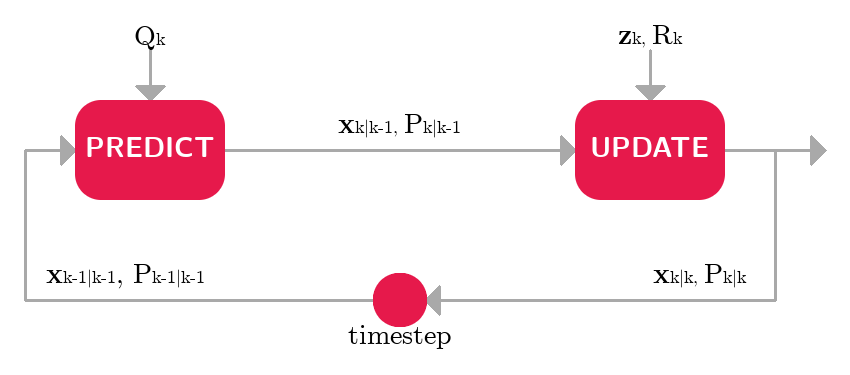
\includegraphics[scale=0.50]{ekf_diagram}
        \caption{\label{fig:ekf_diagram} System diagram showing the EKF process to estimate a state vector $\mathbf{x}_{k|k}$ and its covariance matrix $P_{k|k}$ from $\mathbf{x}_{k-1|k-1}$, $P_{k-1|k-1}$ and $\mathbf{z}_k$ with noise matrices $Q_k$ and $R_k$.}
    \end{figure}
    
where $\mathbf{u}_k$ is the control vector and $\mathbf{w}_k$ and $\mathbf{v}_k$ are the errors in the measurement process, which are assumed to be Gaussian noises with an average of zero and with covariance matrices $Q_k$ and $R_k$ respectively.
For the purposes of this project the control vector $\mathbf{u}_k$ is left as $\mathbf{0}$ considered that it denotes user input, which isn't present in this model.

A note on the notation: $k_1|k_2$ refers to state in step $k_1$ given the information known in step $k_2$, where $k_1$ and $k_2$ are arbitrary steps.
Based on this, $\mathbf{x}_{k|k-1}$ is the state vector $\mathbf{x}$ in step $k$ knowing the information from $k-1$.
The exact logic on how this is updated is related to the measurement vector and is explained later in this section.

The transition and observation matrices $J_{\mathbf{f}(k)}$ and $J_{\mathbf{h}(k)}$ are also defined as the following Jacobian matrices:
    \begin{align*}
        J_{\mathbf{f}(k)} &= \frac{\partial \mathbf{f}}{\partial \mathbf{x}}\Bigr|_{\substack{\mathbf{\hat{x}}_{k-1|k-1}}}\\
        J_{\mathbf{h}(k)} &= \frac{\partial \mathbf{h}}{\partial \mathbf{z}}\Bigr|_{\substack{\mathbf{z}_{k}}}\,.
    \end{align*}

\newpage

To calculate the computational complexity of the algorithm, the size of the state vector $\mathbf{x}_k$ is first defined as $n$ and the size of the measurement vector $\mathbf{z}_k$ as $m$, while also defining the computational cost of applying the functions $\mathbf{f(\mathbf{x}, \mathbf{u})}$ and $\mathbf{h}(\mathbf{x})$ on an arbitrary input as $\text{C}(\mathbf{f}(\cdot,\cdot))$ and $\text{C}(\mathbf{h}(\cdot))$ respectively.

% \newpage

To obtain the next state two steps are required, \textbf{Predict} and \textbf{Update}.
The former requires the following computations to obtain the estimate $\mathbf{\hat{x}}_{k|k-1}$ and the covariance matrix $P_{k|k-1}$ \textit{a priori}:
    \begin{align*}
        \mathbf{\hat{x}}_{k|k-1} &= \mathbf{f}(\mathbf{\hat{x}}_{k-1|k-1}, \mathbf{u}_k) &\rightarrow \text{C}(\mathbf{f}(\cdot, \cdot))\\
        P_{k|k-1} &= J_{\mathbf{f}(k)} P_{k-1|k-1} J_{\mathbf{f}(k)}^T + Q_k &\rightarrow 2n^3 + n^2\,,
    \end{align*}

Then, to calculate the estimated state $\mathbf{\hat{x}}_{k|k}$ and the covariance matrix $P_{k|k}$ \textit{a posteriori}, the following calculations are done in the latter step:
    \begin{align}
        \nonumber &\mathbf{\tilde{y}}_k = \mathbf{z}_k - \mathbf{h}(\mathbf{\hat{x}}_{k|k-1}) &\rightarrow m + \text{C}(\mathbf{h}(\cdot))\\
        &S_k = J_{\mathbf{h}(k)} P_{k|k-1} J_{\mathbf{h}(k)}^T + R_k &\rightarrow n^2m + nm^2 + m^2 \label{eq:ekf_Sk}\\
        &K_k = P_{k|k-1} J_{\mathbf{h}(k)}^T S_k^{-1} &\rightarrow n^2m + nm^2\label{eq:ekf_Kk}\\
        \nonumber &\mathbf{\hat{x}}_{k|k} = \mathbf{\hat{x}}_{k|k-1} + K_k \mathbf{\tilde{y}}_k &\rightarrow nm + m\\
        &P_{k|k} = (I - K_k J_{\mathbf{h}(k)}) P_{k|k-1} &\rightarrow n^2m + n^2\,,\label{eq:ekf_Pk}
    \end{align}
where $\mathbf{\tilde{y}}_k$ is the called residual measurement of the step $k$, $S_k$ is its covariance matrix, named residual covariance matrix, and $K_k$ is defined as the Kalman gain during that step.
The Kalman gain is a matrix of gain from each measurement to each estimation, and if it's zero then $\mathbf{x}_{k|k} = \mathbf{x}_{k|k-1}$.

To calculate the computational complexity of each step, it is assumed that the complexity of multiplying two matrices of the same size $p\times p$ is $O(p^3)$, multiplying matrices of sizes $p\times q$ and $q\times r$ is $O(p\,q\,r)$ and inverting a matrix of size $p\times p$ has a complexity of $O(p^3)$.
Considering that the computation of $P_{k|k-1} (J_h)_k^T$ in step \eqref{eq:ekf_Sk} is reused in step \eqref{eq:ekf_Kk}, the total complexity at an arbitrary step $k$ of the algorithm is the following:
    \begin{align*}
        \text{C}(\mathbf{f}(\cdot, \cdot)) + \text{C}(\mathbf{h}(\cdot)) + 2n^3 + 2n^2(1+m) \\+ n(1+m+2m^2) + m(1+m)\,,
    \end{align*}
and in Big O notation:
    \begin{align}
        \text{O}(\text{C}(\mathbf{f}(\cdot, \cdot)) + \text{C}(\mathbf{h}(\cdot)) + n^3 + n^2m + nm^2)\,.
    \end{align}
\newpage
\subsection{Track Finding} \label{ssec:framework_tf}
In the Drift Chambers software, each particle's track is estimated independently via the EKF, process that is dubbed \textbf{Track Fitting}.
The state vector estimated by the EKF is $\mathbf{x}_k(z)$, and is defined as:
    \begin{equation*}
        \mathbf{x}_k(z) = \begin{pmatrix}x\\ y\\ \theta_x\\ \theta_y\\ q\end{pmatrix}\,,
    \end{equation*}
given that:
    \begin{equation*}
        \theta_x = \frac{\text{p}_x}{\text{p}_z},
        \theta_y = \frac{\text{p}_y}{\text{p}_z},
        q = \frac{Q_e}{\|\mathbf{p}\|}\,,
    \end{equation*}
    
where ($x,y$) represents the coordinates of the particle measured in a specific plane $z$, commonly denominated \textbf{measurement plane}.
A measurement plane $z$ can be thought of as a plane perpendicular to the beam line seen in Figure \ref{fig:dc_horizontal_cut} producing a view similar to the one seen in Figure \ref{fig:dc_vertical_cut}.
Unlike traditional methods, $z$ is used as the ``time'' variable because the speed of each particle in $z$ is constant for this purpose.
$\mathbf{p}=(p_x,p_y,p_z)$ is the momentum of the particle in that measurement plane and $Q_e$ is the electric charge of the particle. The equations of motion
% , expressed as derivatives with respect to $z$, 
are:
    \begin{align*}
        f_x(z, \mathbf{x}) &= \theta_x\\
        f_y(z, \mathbf{x}) &= \theta_y\\
        \nonumber f_{\theta_x}(z, \mathbf{x}) &= q\, v \sqrt{1+\theta_x^2+\theta_y^2}\\
        &~~\left(\theta_y(\theta_x \operatorname{B_{1}}(x,y,z)+\operatorname{B_{3}}(x,y,z) - (1+\theta_x^2) \operatorname{B_{2}}(x,y,z)\right)\\
        \nonumber f_{\theta_y}(z, \mathbf{x}) &= q\, v \sqrt{1+\theta_x^2+\theta_y^2}\\ 
        &~~\left(-\theta_x (\theta_y\, \operatorname{B_{2}}(x,y,z)+\operatorname{B_{3}}(x,y,z) + (1+\theta_y^2) \operatorname{B_{1}}(x,y,z)\right)\\
        f_q(z, \mathbf{x}) &= 0\,,
    \end{align*}

where $\textbf{B}(x,y,z) = (\operatorname{B_{1}}(x,y,z), \operatorname{B_{2}}(x,y,z), \operatorname{B_{3}}(x,y,z))$ is the effect of the magnetic field in a particular $(x,y,z)$ position inside the detector and $v$ is the speed of light in the medium.
The components of $\textbf{B}$ are defined as $\operatorname{B_{1}}$, $\operatorname{B_{2}}$ and $\operatorname{B_{3}}$ instead of $\operatorname{B_{x}}$, $\operatorname{B_{y}}$ and $\operatorname{B_{z}}$ to avoid confusion with the notation of partial derivatives.
For the EKF to be able to be solved, the gradient of these equations of motion are also obtained:
    \begin{align*}
        \frac{\partial f_x}{\partial x} = 0,~
        \frac{\partial f_x}{\partial y} = 0,~
        \frac{\partial f_x}{\partial \theta_x} &= 1,~
        \frac{\partial f_x}{\partial \theta_y} = 0,~
        \frac{\partial f_x}{\partial q} = 0\\
        \frac{\partial f_y}{\partial x} = 0,~
        \frac{\partial f_y}{\partial y} = 0,~
        \frac{\partial f_y}{\partial \theta_x} &= 0,~
        \frac{\partial f_y}{\partial \theta_y} = 1,~
        \frac{\partial f_y}{\partial q} = 0\,,
    \end{align*}
    \begin{align}
        \frac{\partial f_{\theta_x}}{\partial x} &= 
        q\, v \sqrt{\theta_{x}^{2} + \theta_{y}^{2} + 1} \nonumber\\ 
        &~~\left(\theta_{y} \left(\theta_{x} \frac{\partial}{\partial x} \operatorname{B_{1}}{\left (x,y,z \right)} + \frac{\partial}{\partial x} \operatorname{B_{3}}{\left (x,y,z \right )}\right) + \left(- \theta_{x}^{2} - 1\right) \frac{\partial}{\partial x} \operatorname{B_{2}}{\left (x,y,z \right )}\right) \label{eq:tf_dtx_dx}\\
        \frac{\partial f_{\theta_x}}{\partial y} &=
        q\, v \sqrt{\theta_{x}^{2} + \theta_{y}^{2} + 1} \nonumber\\
        &~~\left(\theta_{y} \left(\theta_{x} \frac{\partial}{\partial y} \operatorname{B_{1}}{\left (x,y,z \right )} + \frac{\partial}{\partial y} \operatorname{B_{3}}{\left (x,y,z \right )}\right) + \left(- \theta_{x}^{2} - 1\right) \frac{\partial}{\partial y} \operatorname{B_{2}}{\left (x,y,z \right )}\right) \label{eq:tf_dtx_dy}\\
        \frac{\partial f_{\theta_x}}{\partial \theta_x} &=
        \frac{q\, \theta_{x}\, v \left(\theta_{y} \left(\theta_{x} \operatorname{B_{1}}{\left (x,y,z \right )} + \operatorname{B_{3}}{\left (x,y,z \right )}\right) - \left(\theta_{x}^{2} + 1\right) \operatorname{B_{2}}{\left (x,y,z \right )}\right)}{\sqrt{\theta_{x}^{2} + \theta_{y}^{2} + 1}} \nonumber\\
        &~~ + q\, v \left(- 2 \theta_{x} \operatorname{B_{2}}{\left (x,y,z \right )} + \theta_{y} \operatorname{B_{1}}{\left (x,y,z \right )}\right) \sqrt{\theta_{x}^{2} + \theta_{y}^{2} + 1} \nonumber\\
        \frac{\partial f_{\theta_x}}{\partial \theta_y} &=
        \frac{q\, \theta_{y}\, v \left(\theta_{y} \left(\theta_{x} \operatorname{B_{1}}{\left (x,y,z \right )} + \operatorname{B_{3}}{\left (x,y,z \right )}\right) - \left(\theta_{x}^{2} + 1\right) \operatorname{B_{2}}{\left (x,y,z \right )}\right)}{\sqrt{\theta_{x}^{2} + \theta_{y}^{2} + 1}} \nonumber\\
        &~~ + q\, v \left(\theta_{x} \operatorname{B_{1}}{\left (x,y,z \right )} + \operatorname{B_{3}}{\left (x,y,z \right )}\right) \sqrt{\theta_{x}^{2} + \theta_{y}^{2} + 1} \nonumber\\
        \frac{\partial f_{\theta_x}}{\partial q} &=
        v \left(\theta_{y} \left(\theta_{x} \operatorname{B_{1}}{\left (x,y,z \right )} + \operatorname{B_{3}}{\left (x,y,z \right )}\right) - \left(\theta_{x}^{2} + 1\right) \operatorname{B_{2}}{\left (x,y,z \right )}\right) \sqrt{\theta_{x}^{2} + \theta_{y}^{2} + 1} \nonumber
    \end{align}
    \begin{align}
        \frac{\partial f_{\theta_y}}{\partial x} &=
        q\,v \sqrt{\theta_{x}^{2} + \theta_{y}^{2} + 1} \nonumber\\
        &~~ \left(- \theta_{x} \left(\theta_{y} \frac{\partial}{\partial x} \operatorname{B_{2}}{\left (x,y,z \right )} + \frac{\partial}{\partial x} \operatorname{B_{3}}{\left (x,y,z \right )}\right) + \left(\theta_{y}^{2} + 1\right) \frac{\partial}{\partial x} \operatorname{B_{1}}{\left (x,y,z \right )}\right) \label{eq:tf_dty_dx}\\
        \frac{\partial f_{\theta_y}}{\partial y} &=
        q\, v \sqrt{\theta_{x}^{2} + \theta_{y}^{2} + 1} \nonumber\\
        &~~ \left(- \theta_{x} \left(\theta_{y} \frac{\partial}{\partial y} \operatorname{B_{2}}{\left (x,y,z \right )} + \frac{\partial}{\partial y} \operatorname{B_{3}}{\left (x,y,z \right )}\right) + \left(\theta_{y}^{2} + 1\right) \frac{\partial}{\partial y} \operatorname{B_{1}}{\left (x,y,z \right )}\right) \label{eq:tf_dty_dy}\\
        \frac{\partial f_{\theta_y}}{\partial \theta_x} &=
        \frac{q\, \theta_{x}\, v \left(- \theta_{x} \left(\theta_{y} \operatorname{B_{2}}{\left (x,y,z \right )} + \operatorname{B_{3}}{\left (x,y,z \right )}\right) + \left(\theta_{y}^{2} + 1\right) \operatorname{B_{1}}{\left (x,y,z \right )}\right)}{\sqrt{\theta_{x}^{2} + \theta_{y}^{2} + 1}}  \nonumber\\
        &~~ + q\, v \left(- \theta_{y} \operatorname{B_{2}}{\left (x,y,z \right )} - \operatorname{B_{3}}{\left (x,y,z \right )}\right) \sqrt{\theta_{x}^{2} + \theta_{y}^{2} + 1} \nonumber\\
        \frac{\partial f_{\theta_y}}{\partial \theta_y} &=
        \frac{q\, \theta_{y}\, v \left(- \theta_{x} \left(\theta_{y} \operatorname{B_{2}}{\left (x,y,z \right )} + \operatorname{B_{3}}{\left (x,y,z \right )}\right) + \left(\theta_{y}^{2} + 1\right) \operatorname{B_{1}}{\left (x,y,z \right )}\right)}{\sqrt{\theta_{x}^{2} + \theta_{y}^{2} + 1}} \nonumber\\
        &~~ + q\, v \left(- \theta_{x} \operatorname{B_{2}}{\left (x,y,z \right )} + 2 \theta_{y} \operatorname{B_{1}}{\left (x,y,z \right )}\right) \sqrt{\theta_{x}^{2} + \theta_{y}^{2} + 1} \nonumber\\
        \frac{\partial f_{\theta_y}}{\partial q} &=
        v \left(- \theta_{x} \left(\theta_{y} \operatorname{B_{2}}{\left (x,y,z \right )} + \operatorname{B_{3}}{\left (x,y,z \right )}\right) + \left(\theta_{y}^{2} + 1\right) \operatorname{B_{1}}{\left (x,y,z \right )}\right) \sqrt{\theta_{x}^{2} + \theta_{y}^{2} + 1} \nonumber
    \end{align}
    \begin{equation*}
        \frac{\partial f_q}{\partial x} = 0,~
        \frac{\partial f_q}{\partial y} = 0,~
        \frac{\partial f_q}{\partial \theta_x} = 0,~
        \frac{\partial f_q}{\partial \theta_y} = 0,~
        \frac{\partial f_q}{\partial q} = 0\,.
    \end{equation*}

\newpage

It's worth noting that $\frac{\partial \textbf{B}}{\partial x}$, $\frac{\partial \textbf{B}}{\partial y}$ and $\frac{\partial \textbf{B}}{\partial z}$ are in practice very small.
Due to this, Equations \eqref{eq:tf_dtx_dx}, \eqref{eq:tf_dtx_dy}, \eqref{eq:tf_dty_dx} and \eqref{eq:tf_dty_dy} are redefined as:
    \begin{equation*}
        \frac{\partial f_{\theta_x}}{\partial x} = 0, ~
        \frac{\partial f_{\theta_x}}{\partial y} = 0, ~
        \frac{\partial f_{\theta_y}}{\partial x} = 0, ~
        \frac{\partial f_{\theta_y}}{\partial y} = 0\,.
    \end{equation*}
All of these equations of motions are then solved via Runge Kutta 4 as explained in Section \ref{ssec:framework_rk4}.

After transporting from one measurement plane to the next, EKF's \textbf{Update} phase must be applied.
The input state vector is again the same $\mathbf{x_{k|k-1}}$, with its related covariance matrix denoted as $P_{k|k-1}$, and the measurement vector $\mathbf{z}_k$, for each measurement plane $z$, is defined as:
    \begin{equation*}
        \mathbf{z}_k(z) = \begin{pmatrix}x_m\\ u\\ t\\ l\\ w\end{pmatrix}\,,
    \end{equation*}

A measurement results from an effective hit to a particular wire where a local tilted coordinate system is defined in which $y=0$ for convenience.
Each of the scalar components denote different attributes related to the measurement itself:
    \begin{itemize}
        \item $x_m$: \textbf{measured $x$ at $z$}.
        Note that since $y$ is fixed to $0$ and the measurement plane $z$ is known, only $x$ needs to be measured.
        \item $u$: \textbf{uncertainty of the measurement}.
        Converting the time to distance from the moment the measurement is taken at the wire, a certain statistical uncertainty is related to the measurement, with a minimum close to $300$ [ns].
        \item $t$: \textbf{measurement tilt}.
        Tilt used to define the tilted coordinate system which can be either $30\degree$ or $-30\degree$.
        \item $l$: \textbf{length of the wire from which the measurement is obtained}.
        As can be seen in Figure \ref{fig:dc_vertical_cut} from Section \ref{ssec:framework_dc}, each superlayer in each sector has an isosceles trapezoid shape when viewed transverse to the beam line at the target location.
        This means that wires can have different lengths depending on where on the trapezoid they're strung, so this needs to be considered when using the measurements.
        \item $w$: \textbf{the wire's maximum sag}.
        This variable denotes the maximum possible sag caused by the catenary the wire naturally follows due to gravity.
    \end{itemize}
then, vector $\mathbf{h}_k(z)$ is computed:
    \begin{equation} \label{eq:framework_tf_h}
        \mathbf{h}_k(z) = \begin{pmatrix}1\\ -\text{tan}(t) - \frac{4w}{l} \cdot (1 - \frac{2y}{l})\\ 0\\ 0\\ 0\end{pmatrix}\,,
    \end{equation}
which is a vector used to define the transformation necessary to project the state vector into the local coordinate system of the measurement.

A $H_k$ matrix can then be computed from $\mathbf{h}_k(z)$ to update the covariance matrix:
    \begin{equation*}
        H_k = \mathbf{h}_k \mathbf{h}_k^T\,,
    \end{equation*}
then, to calculate the filtered covariance matrix $P_{k|k}$:
    \begin{equation*}
        P_{k|k} = \left( P_{k|k-1}^{-1} + \frac{H_k}{|u|} \right)^{-1}\,,
    \end{equation*}

From this new covariance matrix, a vector $\mathbf{k}_k$ can be computed:
    \begin{equation*}
        \mathbf{k}_k = \frac{P_{k|k} \times \mathbf{h}_k}{|u|}\,,
    \end{equation*}
using $\mathbf{h}_k(z)$ from Equation \eqref{eq:framework_tf_h}.
From this vector $\mathbf{k}_k$, both the state vector $\mathbf{x}_{k|k}$ and the quadratic error $\chi^2_k$ (described in Appendix \ref{add:errors}) can be obtained:
    \begin{align*}
        \mathbf{x}_{k|k} &= \mathbf{x}_{k|k-1} + (x_m - (x - h_{k(2)})) \cdot \mathbf{k}_k\\
        \chi^2_k &= \chi^2_{k-1} + \frac{(x_m - (x - h_{k(2)}))^2}{|u|}\,,
    \end{align*}
where $h_{k(2)}$ is the second scalar component of the vector $\mathbf{h}_k(z)$ from Equation \eqref{eq:framework_tf_h}.
The quadratic error obtained can be used to evaluate how well the fit is going and, when the EKF is finished, to measure the quality of the fit.

The pseudocode for this particular implementation of the EKF for CLAS12 is presented:

\newpage

    \begin{algorithm}[H]
        \caption{Kalman Filter}
        \SetAlgoLined
        \DontPrintSemicolon
        \SetKwProg{Def}{def}{:}{}
        $Z \gets$ array of measurement planes\;
        $m \gets$ array of measurements\;
        $\mathbf{s}_0 \gets$ initial state vector\;
        $S_0 \gets$ initial covariance matrix\;
        $I \gets$ total number of iterations\;
    
        \Def{\upshape run\_fitter$(Z, m, \mathbf{s}, S, I)$}{
            $\chi_b^2 \gets\infty$\;
            $K \gets \text{size}(Z)-1$\;
            \For{$i\gets0$ \KwTo $I$}{
                $\chi_c^2 \gets0$\;
                \uIf{$i > 0$}{
                    $\mathbf{s}_0, S_0 \gets \text{transport}(K, 0, \mathbf{s}_K, S_K, \chi_c^2, Z)$\;
                }
                \For{$k\gets0$ \KwTo $K$}{
                    $\mathbf{s}_{k+1}, S_{k+1} \gets \text{transport}(k, k+1, \mathbf{s}_k, S_k, Z)$\;
                    $\mathbf{s}_{k+1}, S_{k+1}, \chi_c^2 \gets \text{filter}(\mathbf{s}_{k+1}, S_{k+1}, m_{k+1}, \chi_c^2)$\;
                }
                \uIf{\upshape $|\mathbf{s}_b.Q-\mathbf{s}_K.Q| < 5\cdot10^{-4}$ and 
                    $|\mathbf{s}_b.x-\mathbf{s}_K.x| < 10^{-4}$ and 
                    $|\mathbf{s}_b.y-\mathbf{s}_K.x| < 10^{-4}$ and 
                    $|\mathbf{s}_b.\theta_x-\mathbf{s}_K.\theta_x| < 10^{-6}$ and 
                    $|\mathbf{s}_b.\theta_y-\mathbf{s}_K.\theta_y| < 10^{-6}$}{
                    $i = I$\;
                }
                \uIf{$\chi_c^2 < \chi_b^2$}{
                    $\chi_b^2 \gets \chi_c^2$\;
                    $\mathbf{s}_b \gets \mathbf{s}_K$\;
                }
            }
            % $\chi^2 \gets \text{getFinalChi2()}$ % Note: Describing this is really hard and probably worth less than its benefit imo.
            \Return{$\mathbf{s}_K$, $S_K$, $\chi_b^2$}
        }
    \end{algorithm}
    
\newpage

    \begin{algorithm}[H]
        \caption{Transport}
        \SetAlgoLined
        \DontPrintSemicolon
        \SetKwProg{Def}{def}{:}{}
        $i \gets$ initial state ($k-1|k-1$)\;
        $f \gets$ final state ($k|k-1$)\;
        $\mathbf{s}_i \gets$ state vector at $i$\;
        $S_i \gets$ covariance matrix at $i$\;
        $\chi^2 \gets \chi^2$ error\;
        $Z \gets$ array of measurement planes\;
        \Def{\upshape transport$(i, f, \mathbf{s}_i, S_i, \chi^2, Z)$}{
            $\mathbf{s}_f \gets \mathbf{s}_i$\;
            $S_f \gets S_i$\;
            $h \gets 1$ \CommentSty{// step size}\;
            $z \gets Z_i$\;
            % $a \gets \text{sign}(Z_f - Z_i)$\;
            \While{\upshape $\text{sign}(Z_f - Z_i)\cdot \mathbf{s}_f.z < \text{sign}(Z_f - Z_i)\cdot Z_f$}{
                $h_{\text{signed}} \gets \text{sign}(Z_f - Z_i)\cdot h$\;
                \uIf{\upshape $\text{sign}(Z_f - Z_i)\cdot (\mathbf{s}_f.z + h_{\text{signed}}) > \text{sign}(Z_f - Z_i)\cdot Z_f$}{
                    $h_{\text{signed}} \gets \text{sign}(Z_f - Z_i)\cdot |Z_f - \mathbf{s}_f.z|$\;
                }
                $z, \mathbf{s}_f, S_f, \chi^2 \gets \text{rk4\_transport}(z, h_{\text{signed}}, \mathbf{s}_f, S_f, \chi^2)$\;
            }
            \Return{$\mathbf{s}_f$, $S_f$}
        }
    \end{algorithm}

    \begin{algorithm}[H]
        \caption{Filter}
        \SetAlgoLined
        \DontPrintSemicolon
        \SetKwProg{Def}{def}{:}{}
        $\mathbf{s}_i \gets$ state vector at $i$ ($k|k-1$)\;
        $S_i \gets$ covariance matrix at $i$ ($k|k-1$)\;
        $\mathbf{m}_k \gets$ measurement vector at $k$\;
        $\chi^2 \gets \chi^2$ error before running the filter\;
        \Def{\upshape filter$(\mathbf{s}_i, S_i, \mathbf{m}_k, \chi^2)$}{
            $\mathbf{h} \gets \text{get\_h}(\mathbf{s}_i.y, \mathbf{m}_k.t, \mathbf{m}_k.w, \mathbf{m}_k.l)$\;
            $S_f \gets S_i - \frac{S_i\mathbf{h}\mathbf{h}^TS_i}{1 + \mathbf{h}^TS_i\mathbf{h}}$\;
            $\mathbf{k} \gets <0, 0, 0, 0, 0>$\;
            \For{$j \gets 1$ \KwTo $5$}{
                $k_j \gets \frac{(h_0\cdot S_{f(j,0)} + h_1\cdot S_{f(j,1)})}{|\mathbf{m}_k.u|}$\;
            }
            $c \gets \text{get\_correction}(\mathbf{s}_i.x, \mathbf{s}_i.y, \mathbf{m}_k.t, \mathbf{m}_k.w, \mathbf{m}_k.l)$\;
            $\chi^2 \gets \chi^2 + \frac{(\mathbf{m}_k.x - c)^2}{|\mathbf{m}_k.u|}$\;
            $\mathbf{s}_f \gets \mathbf{s}_i + \mathbf{k}\cdot (\mathbf{m}_k.x - c)$\;
            \Return{$\mathbf{s}_f$, $S_f$, $\chi^2$}
        }
        \Def{\upshape get\_h$(y,t,w,l)$}{
            \Return{$<1, -\tan(6t) - w\cdot\frac{4}{l}\cdot\big(1-\frac{2y}{l}\big), 0, 0, 0>$}
        }
        \Def{\upshape get\_correction$(x,y,t,w,l)$}{
            \Return{$x - \tan(6t)\cdot y - w\cdot\big(1-\frac{2y}{l}\big)^2$}
        }
    \end{algorithm}
\newpage
\subsection{Fourth Order Runge Kutta} \label{ssec:framework_rk4} 
The Fourth Order Runge Kutta method or simply Runge Kutta 4 (RK4) is an iterative method used to solve initial value problems, originally proposed by Carl Runge and Wilhelm Kutta~\cite{runge1895numerische}.
In CLAS12, the method is used to estimate a state vector $\mathbf{x}(z+h)$ between two measurement planes $z_{k-1}$ and $z_k$, denoted as $z_{k-1} + h$, where $h$ is the step size used, given that $z_k > z_{k-1} + h$, and thus $\mathbf{x}(z+h)$ is between $\mathbf{x}_{k-1|k-1}$ and $\mathbf{x}_{k|k-1}$.

Let an initial value problem for estimating $\mathbf{x}(z+h)$ be:
    \begin{equation*}
        \mathbf{\dot{x}} = \mathbf{f}(z,\mathbf{x}), \mathbf{x}(z_0) = \mathbf{x}_0\,,
    \end{equation*}
where $\mathbf{x}$ is the unknown vector function of the measurement plane $z$ to be approximated, $\mathbf{\dot{x}}$ is its rate of change, defined as a function of $z$ and $\mathbf{x}$ itself.
$\mathbf{f}$ denotes the equations of motion from Section \ref{ssec:framework_tf} and the initial $z_0$ and $\mathbf{x}_0$ are given.
Using the step size $h > 0$ defined before:
    \begin{equation}
        \mathbf{x}(z+h) = \mathbf{x}(z) + \frac{1}{6}(\mathbf{r}_1 + \mathbf{r}_2 + \mathbf{r}_3 + \mathbf{r}_4)\,,\label{eq:framework_rk4_x}
    \end{equation}
with $\mathbf{r}_1$, $\mathbf{r}_2$, $\mathbf{r}_3$ and $\mathbf{r}_4$ defined as:
    \begin{align*}
        \mathbf{r}_1 &= h\cdot\mathbf{f}(z, \mathbf{x}(z))\,,\\
        \mathbf{r}_2 &= h\cdot\mathbf{f}\left(z + \frac{h}{2}, \mathbf{x}(z) + \frac{\mathbf{r}_1}{2}\right),\\
        \mathbf{r}_3 &= h\cdot\mathbf{f}\left(z + \frac{h}{2}, \mathbf{x}(z) + \frac{\mathbf{r}_2}{2}\right),\\
        \mathbf{r}_4 &= h\cdot\mathbf{f}(z + h, \mathbf{x}(z) + \mathbf{r}_3)\,.
    \end{align*}
Finally, the $\mathbf{x}(z+h)$ presented in Equation \eqref{eq:framework_rk4_x} is named the RK4 approximation of $\mathbf{x}(z+h)$~\cite{sauer2012numerical}.

The pseudocode for the implementation of RK4 at the DC software is presented:

\newpage

    \begin{algorithm}[H]
        \caption{Runge Kutta 4}
        \SetAlgoLined
        \DontPrintSemicolon
        \SetKwProg{Def}{def}{:}{}
        $z \gets$ initial measurement location\;
        $h \gets$ step size\;
        $\mathbf{s}_k \gets$ state vector at $k$\;
        $S_k \gets$ covariance matrix at $k$\;
        $\chi^2 \gets \chi^2$ error\;
        \Def{\upshape rk4\_transport$(z, h, \mathbf{s}_k, S_k, \chi^2)$}{
            \CommentSty{// $r_1$}\;
            $\mathbf{B} \gets$ bfield at location\;
            $\mathbf{k}_{\mathbf{x}(1)} \gets \mathbf{f}_{\mathbf{x}}(z, \mathbf{x}, \mathbf{B})$\;
            $K_{J(1)} \gets F_J(z, \mathbf{x}, J, \mathbf{B})$\;
            \CommentSty{// $r_2$}\;
            $\mathbf{B} \gets$ bfield at new location\;
            $\mathbf{k}_{\mathbf{x}(2)} \gets \mathbf{f}_{\mathbf{x}}(z+\frac{h}{2}, \mathbf{x}+\frac{h}{2}\mathbf{k}_{\mathbf{x}(1)}, \mathbf{B})$\;
            $K_{J(2)} \gets F_J(z+\frac{h}{2}, \mathbf{x}+\frac{h}{2}\mathbf{k}_{\mathbf{x}(1)}, J+\frac{h}{2}K_{J(1)}, \mathbf{B})$\;
            \CommentSty{// $r_3$}\;
            $\mathbf{B} \gets$ bfield at new location\;
            $\mathbf{k}_{\mathbf{x}(3)} \gets \mathbf{f}_{\mathbf{x}}(z+\frac{h}{2}, \mathbf{x}+\frac{h}{2}\mathbf{k}_{\mathbf{x}(2)}, \mathbf{B})$\;
            $K_{J(3)} \gets F_J(z+\frac{h}{2}, \mathbf{x}+\frac{h}{2}\mathbf{k}_{\mathbf{x}(2)}, J+\frac{h}{2}K_{J(2)}, \mathbf{B})$\;
            \CommentSty{// $r_4$}\;
            $\mathbf{B} \gets$ bfield at new location\;
            $\mathbf{k}_{\mathbf{x}(4)} \gets \mathbf{f}_{\mathbf{x}}(z+h, \mathbf{x}+h\mathbf{k}_{\mathbf{x}(3)}, \mathbf{B})$\;
            $K_{J(4)} \gets F_J(z+h, \mathbf{x}+h\mathbf{k}_{\mathbf{x}(3)}, J+h K_{J(3)}, \mathbf{B})$\;
            \CommentSty{// RK4}\;
            $z \gets z + h$\;
            $\mathbf{x} \gets \mathbf{x} + \frac{h}{6} (\mathbf{k}_{\mathbf{x}(1)} + 2\mathbf{k}_{\mathbf{x}(2)} + 2\mathbf{k}_{\mathbf{x}(3)} + \mathbf{k}_{\mathbf{x}(4)})$\;
            $J \gets J + \frac{h}{6} (K_{J(1)} + 2K_{J(2)} + 2K_{J(3)} + K_{J(4)})$\;
            $S_k \gets$ update\_cov\_mat$(S_k, J)$\;
            $S_k \gets$ q\_process\_estimate$(S_k, z, h, \mathbf{x}, \text{mass})$\;
            \Return{$z,\mathbf{x},S_k,\chi^2$}
        }
    \end{algorithm}
    
where $\mathbf{f}_{\mathbf{x}}(z, \mathbf{x}, \mathbf{B})$ and $F_J(z, \mathbf{x}, J, \mathbf{B})$ are the equations of motion described in Section \ref{ssec:framework_tf}, \texttt{update\_cov\_mat}($S_k, J$) applies the equations of motion of the Jacobian matrix to the covariance matrix and \texttt{q\_process\_estimate}($S_k, z, h, \mathbf{x}, \text{mass}$) updates it from the estimated noise in $q$.
More detail on this can be seen in the original source code from the repository linked in Appendix \ref{add:code_and_reproducibility}. % Note: There's a spacing issue.
    \newpage
    \secnumbersection{CODE PROFILING} \label{sec:prof}
Since the project consists on the heavy optimization of the DC code, a logical starting point is a detailed profiling of the compiled program in order to figure out where the performance bottlenecks are found so as to focus work on them. % Note: This could use a citation.
Different profiling programs or \textbf{profilers} were evaluated for this purpose, but in the end the default java profiler, or \textbf{jvisualvm}, was used.
A small analysis into the reasoning behind this decision is shown in Section \ref{ssec:prof_tools} and then the profiling results and a short analysis of them is given in Section \ref{ssec:prof_results}.

% DEFINE PROFILING.
Profiling or ``software profiling'' is a dynamic program analysis method that measures all factors to analyze the performance of an application.
These factors were separated into four categories: CPU/GPU usage, memory usage, IO and network operations and database queries.
These categories are used because they encompass all the processes that can be commonly found in an application.

A \textbf{profiler} is a tool that analyzes either the source code or the running program to report its performance after or while it is running, usually offering information like the program's total memory use, the number of times a certain method was called or the largest bottlenecks in the programs execution~\cite{ball1997efficient}.
% EXPLAIN PROFILING VIA SAMPLING VS INSTRUMENTING.
There are three ways to obtain profiling information: \textbf{code instrumentation}, \textbf{statistical sampling} and \textbf{application monitoring}.

\textbf{Code instrumentation} is the act of placing new lines of code in a program and counts how many times they were ran, so as to give the exact number while the program is running or after it is completed~\cite{ball1994optimally}.
Instrumentation can give a very detailed view into exactly how the program is working, but due to the fact that new lines of code are added to the program, the execution time can drastically increase while profiling is taking place.
An important terminological consideration is that code instrumentation is usually simply referred to as profiling, which can lead to confusion when studying the area. % Note: This could use a citation but it comes from reading a lot about the subject online.

In stark contrast, \textbf{statistical sampling} is a less disruptive method that work by stopping the program in regular intervals during its execution, taking a so-called ``snapshot'' and then allowing the application to continue, sacrificing accuracy in favor of speed~\cite{wenisch2006simflex}.
Summarized, sampling may reveal the relative percentage of time spent in frequently-called methods, but cannot provide the exact number of times each method is invoked, unlike instrumentation.

\textbf{Application monitoring} provides a so-called ``eagle's point of view'' onto a running application, focusing on the high-level picture of it.
Monitoring provides very basic information about an application but is the least disruptive of all the methods mentioned, and thus is mostly used for web services that require reports onto how they're running while also minimizing the disruption this analysis has on the running program so as to not impact its performance~\cite{hunt2011java}.

As mentioned before, all of the effort done in this work is based on multiple instances of performance analysis done via the \textbf{jvisualvm} tool.
Also, all the results given in Section \ref{ssec:prof_results} and chapter $6$ are obtained by measuring the total execution time of the program with the tool in a personal computer, an Intel(R) Core(TM) i$5$-$6600$K CPU with $4$ cores running at $3.50$GHz with $8$GB of DDR$4$ $2133$MHz RAM. % CHAPTER REFERENCE
\subsection{Tool Comparison} \label{ssec:prof_tools}
Due to the large significance of the profiling process and its effects on the final results of any analysis, a detailed analysis of the many tools available to profile applications is performed.
They are compared based on four criteria:

    \begin{itemize}
        \item \textbf{CPU Profiling}: How accurate and fast are the sampling and profiling processes available in the application, and if the tool can provide an immediate view into the \textbf{hotspots} in the application.
        A hotspot is the common term used to describe a specific method or code segment that takes up a large portion of the total computation time~\cite{hunt2011java}.
        
        \item \textbf{Memory Analysis}: Since the main focus of the profiling process for this project is the analysis of the CPU time used, the only memory analysis systems required for that purpose are the detection of memory leaks and the count of class instances generated since both of these can impact the computation time.
        A memory leak occurs when object references that are no longer needed are unnecessarily maintained, which is a precise problem related to the java garbage collector~\cite{xu2008precise}.
        
        \item \textbf{Remote Profiling}: Considering that the application will run at the computer facilities at JLab, some of the performance analysis should be done in this environment to assert that the results obtained in a personal computer are correlated to the ones found in it.
        For this, it is crucial that the selected tool allows for remote profiling, so that it is possible to perform analysis locally and remotely.
        
        \item \textbf{License}: Finally, the cost of the profiling application is evaluated to see if the additional features outweigh this price.
    \end{itemize}

\newpage

Using each criterion, the tools analyzed are the default java profiler, \textbf{jvisualvm}, a set of paid tools, \textbf{JProfiler}, \textbf{YourKit}, \textbf{XRebel} and \textbf{JProbe}, and a small set of free applications, including \textbf{Callgrind}, \textbf{Honest Profiler} and \textbf{JIProf}.
While this set is far from comprehensive, the tools analyzed are the ones mainly used in the market as reported in ~\cite{maple2015developer} and ~\cite{maple2015top}, along with various scattered sources.

As mentioned before, it was decided to use \textbf{jvisualvm} due to price restrictions and the fact that it is a robust tool despite being free, contrasted with the fact that the other applications proposed cost at least $\$499$ USD at the time of publication.
Java VisualVM or jvisualvm for short is a graphical user interface that provides tools to profile, monitor and troubleshoot Java applications while they are running on the Java Virtual Machine (JVM)~\cite{java2019jvisualvm}.
The tool was developed by Oracle, the company behind Java, and is provided to programmers for free.
\begin{figure}[ht]
    \centering
    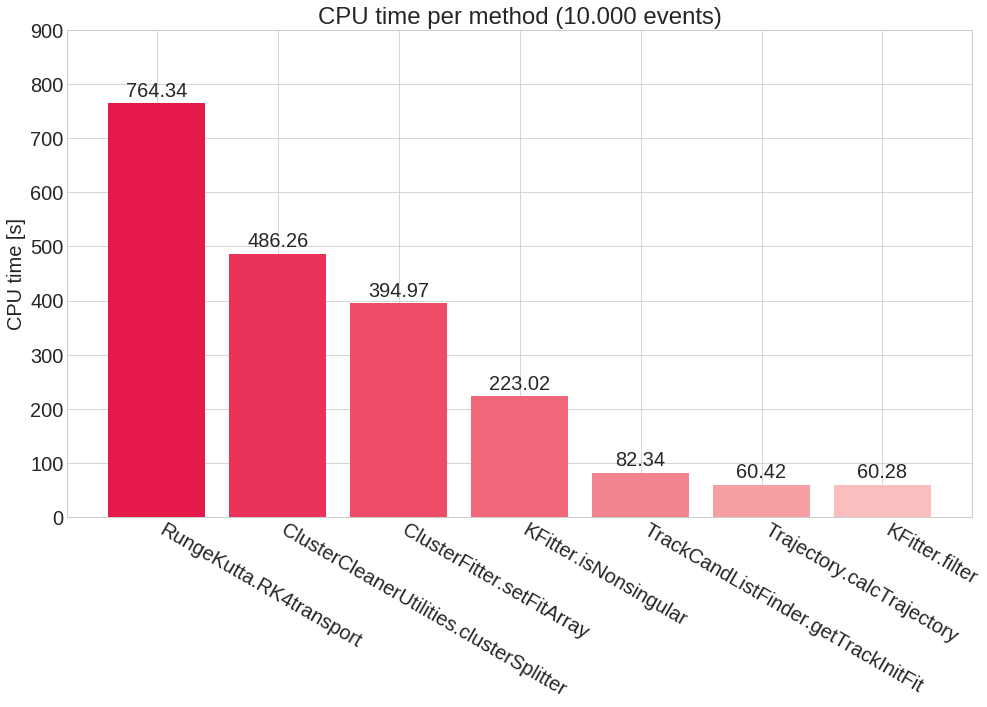
\includegraphics[scale=0.44]{methods_times/1_0.png}
    \caption{\label{fig:methods_times-1_0} Methods' CPU time on the original source code (version $1.0$).}
\end{figure}

\newpage

\subsection{Results} \label{ssec:prof_results}
Using the \textbf{jvisualvm} profiler, the time taken by each component of the CLAS12 offline software can be measured, thus finding the bottlenecks in the execution in order to prioritize work on them.
It's worth noting that all the profiled data presented in this publication is obtained via \textbf{jvisualvm} unless stated otherwise, running the CLAS12 software on $10.000$ events with real experimental data taken from the test file \texttt{clas\_004013.0.hipo}.

As a note before continuing, all figures that relate to profiling information will be always associated to a ``version''.
This is different from the versioning system utilized in the CLAS12 offline software, and is instead one used only in this work to quickly refer to different states of the software after each improvement, and thus, ``version $1.0$'' refers to the initial state of the code, before any changes are made by the author.

The methods taking up more than $2\%$ of the total CPU time before any change is made on the source code is shown in Figure \ref{fig:methods_times-1_0}.
A brief description of the methods in the figure are:

\begin{itemize}
    \item \textbf{Runge Kutta 4}: named \texttt{RK4transport} from the \texttt{RungeKutta} (\texttt{RK4} in Figure \ref{fig:methods_times-1_0}) class, the method is a direct implementation of the algorithm described in Section \ref{ssec:framework_rk4}, taking up a total of $35.1\%$ ($764.34$ seconds) of the total computation time.
    As is explained in detail in Section \ref{ssec:prop_magfield}, most of the time used in this method is taken up by a method to obtain the magnetic field at specific points.
    
    \item \textbf{Cluster Splitter}: named \texttt{clusterSplitter} from the \texttt{CCU} class, which is short for \texttt{ClusterCleanerUtilities}.
    As the name suggests, it refers to the process of splitting the clusters described in Section \ref{ssec:framework_cf} done via the Hough transform, which in simple terms consists of finding line shaped sub-clusters in the split cluster~\cite{hough1962method} and is described in detail in Appendix \ref{add:hough_transform}.
    
    The process is useful because it splits malformed clusters with poor performance to ones that are better fit, but, as can be seen in Figure \ref{fig:methods_times-1_0}, takes $22.4\%$ ($486.26$ seconds) of the total CPU time.
    This is attributed to the fact that it transforms every hit in the original cluster to a so-called ``Hough Space'' to find the split clusters, which is a slow process due to the raw number of hits in each cluster and the number of clusters.

    \item \textbf{Set Fit Array}: named \texttt{setFitArray} from the \texttt{ClusterFitter} (\texttt{CF} in the Figure) class, the method receives clusters and creates arrays from the hits in them which are later fit into a line by the \texttt{fitCluster} method from the same class.
    While the algorithm itself involves only sorting the cluster and then adding them to arrays, the method takes so much time ($18.2\%$ or $394.97$ seconds of the total CPU time) because it's called several times by many methods, especially the \texttt{findHitBasedClusters} method in the \texttt{ClusterFinder} class, and it sorts the cluster for each of these calls.
    
    \item \textbf{Is Nonsingular}: named \texttt{isNonsingular} from the class \texttt{KFitter} (\texttt{KF} in Figure \ref{fig:methods_times-1_0}), it's a method that returns \texttt{true} if a matrix is nonsingular and \texttt{false} otherwise, taking up a total of $10.2\%$ ($223.02$ seconds) of the total computation time.
    The method takes up this much time because it is called twice every time the \texttt{filter} method is called to check if the covariance matrix is singular, and it calculates the determinant of the matrix to do this.
    It's acceleration is discussed in detail in Section \ref{ssec:prop_matrices}.

    \item \textbf{Get Track Initial Fit}: named \texttt{getTrackInitFit} from the \texttt{TCLF} class, short for \texttt{TrackCandListFinder}.
    The method simply provides an initial fit to the Kalman Filter from which to start working, but it takes a total of $3.8\%$ ($82.34$ seconds) mainly due to lack of good programming practices.
    As can be seen later in Section \ref{ssec:val_refactoring_and_optimizations}, the method's time was lowered by a large factor simply by refactoring and applying simple optimizations to the code.
    
    \item \textbf{Calculate Trajectory}: named \texttt{calcTrajectory} from the \texttt{Trajectory} class (\texttt{Traj} in the Figure), this method receives a set of parameters from a track's state vector and, as the name suggests, it calculates and returns an estimated trajectory that the particle described by the vector could take.
    The method's time of $2.8\%$ ($60.42$ seconds) is attributed to the fact that it's ran many times in the code.
    
    \item \textbf{Filter}: represented by the \texttt{filter} method in the \texttt{KFitter} class, it's an implementation of the filtering component of the Kalman filter, described in detail in Section \ref{ssec:framework_ekf}.
    It takes in total of $2.8\%$ ($60.28$ seconds) of the CLAS12 CPU time and its acceleration is described along with the one for \texttt{isNonsingular} in Section \ref{ssec:prop_matrices}.
\end{itemize}

It is worth noting that to obtain the measurements given in this section, the CLAS12 code was profiled in \textbf{jvisualvm} via statistical sampling with a sampling period of $100$ [ms] and by profiling only the packages related to the Drift Chambers (DC): \texttt{org.jlab.service.dc} and \texttt{org.jlab.rec.dc}.
This was done to shorten the profiling sessions time by focusing only on the DC code.
    \newpage
    \secnumbersection{SOLUTION PROPOSAL} \label{sec:prop}

The approach used to improve on the software's computing time followed a logical order.
First, the algorithm is exhaustively analyzed and profiled to find the bottlenecks in the execution, so as to be able to focus the work on them.
Then, the cause for each significant bottleneck is identified and investigated, so as to propose solutions using the state of the art in the field, and after a good understanding of each problem is reached, they are addressed.
Finally, thorough validation sessions are attempted so as to be sure that the changes made don't affect negative the software's results and to secure that the computing time is effectively reduced.

\subsection{Refactoring and Optimizations} \label{ssec:refactoring_and_optimizations} % \subsubsection{Code Clean-up} \label{sssec:cleanup}
Before any large change or algorithm implementation is considered on the software, it was decided to do a so-called ``code-cleanup''.
This was considered necessary mainly because of two reasons:

First, the current implementation had a low readability, presenting various issues like uneven indentation style, non-compliance with the Java code conventions~\cite{sun1997java}, inconsistent and arbitrary variable and method names, among many others.
This can be seen in the link to the original repository provided at Section \ref{add:code_and_reproducibility}.

The second reason is the large presence of many unintentional, unmanaged architectural technical debt (technical debts and their classification are explained briefly in Appendix \ref{add:technical_debt}).
% While most technical debts are invisible without a detailed analysis, the symptoms for many of them can be clear to most experienced programmers.
Many instances of these debts were found in the DC code, in the form of repeated portions of code, a general lack of error checking and reporting and a general lack of comments in difficult-to-understand sections of code, among others.

Due to both these reasons and simply to improve the author's familiarity with the code, the previously mentioned clean-up was done.
The measures implemented in this process are the following:

    \begin{itemize}
        \item \textbf{Addition of comments}: A comprehensive list of the segments of code with a non-intuitive purpose was written.
        A small research was then performed for each point in the list, looking into the math, physics or general algorithms from which it could be derived.
        When this was found, a comment was written either providing a small explanation or referring to the name of the formula or algorithm used.
        When this research was unfruitful, the original author of the code was contacted so that she could provide enough information about the code segment so as to write this explanatory comment (Contact information is given in Appendix \ref{add:code_and_reproducibility}).
    
        Apart from the general comments, a complete JavaDoc documentation was added to the most important classes and methods in the DC code, with sparse documentation added also to hard-to-understand classes or methods in less critical classes.
    
        \item \textbf{Indentation Consistency}: Considering that the indentation style at the DC software was very inconsistent, this was fixed to improve readability.
        Now, the ``ideal length'' of indentations and the use of tab characters or space characters for it has been a long-running debate between programmers, so instead of finding the ``best option'' for it, the current standard used in most of the CLAS12 codebase was implemented, which simply is four space characters per indent.
    
        \item \textbf{Line Length Fixes}: While the code doesn't follow a rigorous standard, a line length of $100$ characters can be seen somewhat consistently thorough the CLAS12 codebase, sticking to the java conventions~\cite{sun1997java}.
        This line length is not strictly applied to the DC code, but instead some extremely long ($>300$ characters) segments of code are separated into various lines to aid readability.
    
        \item \textbf{Class, Method and Variables Names}: The standard Java conventions stipulate a consistent camel case naming standard, and while most of the code follows this style, the DC code tends to stray away from it in many ways.
        These include variables in lower case with or without underscores, variables and methods starting with an underscore, methods starting with uppercase, etc.
        The standard naming convention is applied to all of these instances.
    \end{itemize}

\subsubsection{Refactoring}\label{sssec:refactoring}
By definition, refactoring is the art of safely improving the design of existing code without changing its behaviour.
Changes done to the code through refactoring do not add new functionalities or represent design improvements, but only work to eliminate or reduce \textbf{code \textit{smells}}. % Note: I feel like refactoring does add design improvements but the usual java documentation on this says that by definition they don't so idk.
Code \textit{smells} are warning signs about potential problems in the code, meaning points that are worthy of a revision~\cite{wake2004refactoring}.

A small list of some the code \textit{smells} found in the DC code together with examples and the treatment done follows.
It is worth noting that this list is far from comprehensive, and just lists the \textit{smells} relevant to the discussion:
    \begin{itemize}
        \item \textbf{Long Methods}: Many methods with a very large amount of lines can be found thorough the code.
        In a normal situation this wouldn't be considered to be a big issue, but in the case of DC, many of these large methods contain repeated code or very similar segments, which in itself is considered a problem since it breeds inconsistencies and longer implementation times to any change done to the code.
        
        An example of this is the method \texttt{RK4transport} from the class \texttt{RungeKutta}, from the package \texttt{org.jlab.rec.dc.track.fit}, which is $269$ lines long.
        It's worth mentioning that the algorithm implemented in this method is \textbf{Runge Kutta 4}, and is described in Section \ref{ssec:framework_rk4}.

        The treatment for this problem is easy to implement, and involves simply splitting the method.
        What is done to do this is to extract the repeating segments into their own private methods, allowing then the original method to call these new methods.
        The benefit of this change is the elimination of duplicated code and a large performance improvement due to the elimination of unnecessary loops, which is explained further in Section \ref{sssec:optimizations}.
    
        In the mentioned example, the method can be split into various methods: First, the computation of $k_1$, $k_2$, $k_3$ and $k_4$ can all be done in the same method, reducing $172$ lines of code into $4$ method calls, with the new method being only $45$ lines long.
        After this, the final $RK4$ computation can be left as is, and some extra steps done to compute the covariance matrix can all be split into their own methods, easing the future debugging of the method and allowing each computation to be changed or optimized separately.
        The final \texttt{RK4transport} method is left with a total of $33$ lines of code with $7$ method calls.
        It's worth noting that this number can be further reduced to $20$ lines by packing intermediary variables into arrays, but to avoid the danger of reducing code readability it was considered a good idea to avoid this option.

        \item \textbf{Long Parameter Lists}: Similar to the last \textit{smell}, long parameter lists can be found thorough the DC code.
        In most cases specific to the software in study, these lists are expressed in the form of a long list of inputs for methods.
        An example for this is the \texttt{getTrackInitFit} method in the class \texttt{TrackCandListFinder} contained in the \texttt{org.jlab.rec.dc.track} package, where $20$ parameters are given to the method.
        These parameters are the integer \texttt{sector}, a long list of doubles: \texttt{x1}, \texttt{y1}, \texttt{z1}, \texttt{x2}, \texttt{y2}, \texttt{z2}, \texttt{x3}, \texttt{y3}, \texttt{z3}, \texttt{ux}, \texttt{uy}, \texttt{uz}, \texttt{thX}, \texttt{thY}, \texttt{theta1}, \texttt{theta3}, \texttt{iBdl}, \texttt{TORSCALE}, and an instance of the \texttt{Swim} class.
    
        Fixing such issues is usually easy, just requiring some degree of packaging for the parameters.
        For the example given, the previosly mentioned method is called by \texttt{GetTrackCands}, another method from the same class.
        In this method, three \textbf{cross} objects are unpacked to obtain the first $14$ doubles from the mentioned list, with two more doubles coming from clusters contained in the crosses and finally \texttt{iBdl} coming from the trajectory formed by the crosses.
        These \textbf{cross} objects are sets of two clusters from adjacent superlayers, while the \texttt{iBdl} variables denotes the integral of the magnetic field. % Note: I don't know exactly what iBdl is but no sources I found say more than "Integral of the magnetic field" so at least apparently physicists get it.
        The \texttt{sector} integer mentioned can also be obtained from the first cross.
        As can be seen, the $20$ input parameters given to the method can be replaced with three \texttt{cross} objects, the \texttt{TORSCALE} value and the instance of the \texttt{Swim} class previously mentioned, reducing the parameter list to four objects and only one parameter. % Note: Maybe an UML diagram or something like it might be useful here.
    
        \item \textbf{Commented and Dead Code}: This \textit{smell} consists in the presence of commented code, and is usually caused by either old code that the programmer decided to leave commented instead of deleting in case that it becomes useful in the future.
        Dead code is the phenomena that occurs when new methods are written and old and unused methods are never deleted.
        Both commented and dead code segments are present in large quantities in the DC software, and after a meeting between the author and the programmer it was decided to simply remove all this code since analyzing which segments would be useful or not would probably be too large a task for the minimal benefit provided by doing it.

        \item \textbf{Duplicated Code}: This \textit{smell} is characterized by two or more code fragments that look almost or completely identical.
        Duplication usually occurs when multiple programmers are working on different parts of the same program at the same time, but in the case of the DC software this can be attributed to accidents. % Note: More elaboration here might be useful.
        The solution to this problem is fairly simple: extract the duplicated code, create a new method to run this code and have both instances call this new method.
    
        In the case of the DC software, there is one instance where code duplication is very easily spotted; both the \texttt{RoadFinder} class from the \texttt{org.jlab.rec.dc.trajectory} package and the \texttt{CrossListFinder.TrajectoryParametriz} class from the \texttt{org.jlab.rec.dc.cross} package contain the exact same method, even using the same name, \texttt{evaluate}, and the code in this method does the same: fit a set of points into a line and return the parameters of the fit along with the $\chi^2$ probability and the number of degrees of freedom. % Note: Maybe this paragraph is too angry.
    
        \item \textbf{Data Class}: The final \textit{smell} that will be discussed in this work is the so-called ``data class'' \textit{smell}, which refers to a class that contains only fields and setters and getters to access them.
        In the case of the DC codebase, an example of this would be both the \texttt{StateVec} and the \texttt{CovMat} classes from the \texttt{org.jlab.rec.dc.track.fit} package.
        Both classes just define a state vector (described in Section \ref{ssec:framework_tf}) and a covariance matrix (described in Appendix \ref{add:covariance_matrix}), without providing any methods apart from the basic definition of the concepts.
    
        The treatment for this problem is through the encapsulation of the data class inside another class, ideally one that uses it.
        In the example, both these classes were encapsulated in another class named \texttt{StateVecs} from the same package.
    \end{itemize}

\subsubsection{Optimizations}\label{sssec:optimizations}
While cleaning up and refactoring the code, many optimizations were applied to the critical areas described in Section \ref{ssec:prof_results} so as to accelerate the bottlenecks and speed up the whole CLAS12 software.
These optimizations involve the addition of variables to precompute results instead of calculating them several times, the reduction of complexity orders by removing unnecessary loops, and the improvements brought by simply restructuring the code as described in the last Section.

% Note: Here I could talk about how the precomputation of results helped (and they helped a ton), and how to do the reduction of complexity with examples, especially considering the massive changes in performance this step brought to the code. I'd need some references for this, but I'm afraid I can't find much on that. % TODO: Implement the examples given here in the code.
\newpage
\subsection{Matrices Handling Changes} \label{ssec:prop_matrices}
% NOTE: Maybe this could use a plot?
Based on the profiling analysis shown in Section \ref{ssec:val_refactoring_and_optimizations}, This section focuses on reducing the CPU time of both the \texttt{isNonSingular} and the \texttt{filter} methods, which are explained in the \textbf{Update} segment of Section \ref{ssec:framework_ekf}.
For the calculation of the computational cost of mathematical operations, it is assumed that all ``basic'' operations: summation, subtraction, multiplication and division have a cost of $O(1)$.
The reasoning behind this decision is described in Appendix \ref{add:flops}.

It's worth noting that a very usual approach for accelerating matrix operations at the time of writing is leveraging the computation to GPUs, and it has been commonly used in particular to accelerate the KF itself~\cite{huang2011accelerating,blattner2011performance}.
This approach is not considered useful for CLAS12 because the matrices that are being handled are very small (the covariance matrix is only $5\times5$) and it is easy to realize that the time used to leverage the matrices to a GPU would likely make the software slower than the current implementation due to the time consumed in the memory transfer overhead~\cite{moravanszky2003dense}.

In the same spirit, neither the Strassen~\cite{strassen1969gaussian} or the Coppersmith-Winograd~\cite{coppersmith1990matrix} algorithms are considered to replace matrix multiplications or inversions since they're only useful for large matrices~\cite{ballard2012communication}.
As an example, the actual amount of operations required for computing the Strassen algorithm is $n^2 + n^{2.807}$, which for the case of a $5\times5$ matrix is $\sim117$ contrasted with the $125$ required by the na\"ive implementation and adding additional numerical instability~\cite{ballard2012communication}.
This reduction is small when compared with the specific optimizations that are described below, which eliminate matrix multiplication altogether for the methods brought into attention.

\subsubsection{Matrix Inverse} \label{sssec:prop_matrix_inverse}

To reduce the time spent by the update phase or filter method, the effort was mainly focused in the reduction of the time it takes to calculate the covariance matrix \textit{a posteriori} as seen in Equation \eqref{eq:ekf_Pk}.
The specific implementation of the equation presented in that section for the DC software is the following:

First, the determinant of the covariance matrix $P_{k|k-1}$ is computed and compared with $0$ to drop the track if the matrix is singular or near-singular.
Then, using the measurement data described in Section \ref{ssec:framework_tf}, the vector $\mathbf{h}_k$ is defined as:
    \begin{equation}
        \mathbf{h}_k = \begin{pmatrix}1\\ -\text{tan}(6t) - \frac{4w}{l}(1 - \frac{2y}{l})\\ 0\\ 0\\ 0\end{pmatrix}\,, \label{eq:mhc_hvec}
    \end{equation}
which is simply defined to project the state vector and covariance matrix to the tilted coordinate system from which the measurement is obtained.
From this, the matrix $P_{k|k}$ is computed as:
    \begin{equation}
        P_{k|k} = (P_{k|k-1}^{-1} + H_k)^{-1}\,, \label{eq:mhc_Pk}
    \end{equation}
where $H_k = \mathbf{h}_k^T\mathbf{h}_k$.
Finally, the $P_{k|k}$'s determinant is compared with $0$, again to drop the track if the new covariance matrix is singular.

To reduce the computation time of this calculation, the \textbf{Sherman-Morrison formula} (described in Appendix \ref{add:shermanmorrison_formula}) can be applied as long as $|P_{k|k-1}|\neq 0$~\cite{sherman1950adjustment}.
Applying the formula to Equation \eqref{eq:mhc_Pk}:
    \begin{equation}
        P_{k|k} = P_{k|k-1} - \frac{P_{k|k-1} \mathbf{h}_k \mathbf{h}_k^T P_{k|k-1}}{1 + \mathbf{h}_k^T P_{k|k-1} \mathbf{h}_k}\,. \label{eq:mhc_sm_det}
    \end{equation}
This helps to heavily reduce the total computation time since, as can be seen in the equation, no matrix inversions are required, which are very heavy operations~\cite{fatahalian2004understanding}.
It's worth noting that for this approach to be effective, the order in which the matrix-matrix, matrix-vector and vector-matrix multiplications in Equation \eqref{eq:mhc_sm_det} are applied is of utmost importance, so that no matrix-matrix multiplications are required.
This is done by first multiplying $P_{k|k-1}\cdot \mathbf{h}_k$ and $\mathbf{h}_k^T\cdot P_{k|k-1}$ in the fraction's numerator.

\subsubsection{Determinant Calculation} \label{sssec:prop_det}

To reduce the time spent on checking if the covariance matrices $P_{k|k-1}$ and $P_{k|k}$ are singular, various paths were taken.
First, two alternative ways for computing the matrix's determinant were proposed: The \textbf{Su-Chang formula}~\cite{su1996quick} and a method based on the Cholesky decomposition~\cite{geijn2011notes} of the matrix:

    \begin{itemize}
        \item \textbf{Su-Chang Formula}: The Su-Chang formula is a recursive algorithm that can be used to compute the determinant of a square matrix.
        It is explained in detail in Appendix \ref{add:suchang_formula}.
        As is described by Equation \eqref{eq:suchang_complexity} in the appendix, the number of operations required is $\frac{1}{3}(2n^3 - 3n^2 + 7n - 18)$, in contrast with the usual $n^3$ operations needed to directly compute the determinant using a LU decomposition~\cite{banachiewicz1937berechnung}.
        In the particular case of the KF from CLAS12, considering the covariance matrix's size is of size $5\times5$, the total number of computations required by the Su-Chang formula is $64$, while the direct computation of a determinant using the LU decomposition is $125$.
        
        \item \textbf{Cholesky Decomposition}: Over the real number field, the Cholesky decomposition or factorization is the decomposition of a positive-definite matrix into the product of a lower triangular matrix with its transpose, described in detail in Appendix \ref{add:cholesky_decomp}.
        A na\"ive algorithm implementing the Cholesky decomposition requires $\frac{1}{6}n(2n^2 + 3n + 1)$ operations, with $n-1$ additional operations to multiply the matrix's diagonal and $1$ to compute its square, which leaves the number of operations required at $\frac{1}{6}n(2n^2 + 3n + 7)$.
        For the studied case with $n=5$, the total number of computations required to obtain the matrix's determinant is $60$.
    \end{itemize}

Besides the computation of these three methods separately, another option was evaluated: Hardcoding each alternative.
Considering that the methods only work with a fixed size input matrix ($5\times5)$, it is possible to embed the direct calculation, Su-Chang formula, and Cholesky decomposition methods into the code and optimize the operations required as much as possible.
This optimization was done via reading the expression in algebraic form and counting all the multiplications between $2$ or more variables, returning a list with each one of these combinations along with how many times they were repeated, thus allowing the programmer to add the precomputation of these operations to the code.

It's worth noting that other efforts in this same field exist and are well-known~\cite{pelegri1988optimal,aho1989code} along with their implementations~\cite{fraser1991burg}.
This is because the problem is an instance of the \textbf{C-Reachability problem}, an extension of the \textbf{Reachability} problem often used in compiler construction theory, defined as:

\textit{Given a computational (potentially infinite state) system with a set of allowed rules or transformations with a given associated cost, find the set of rules with the smallest associated cost that reaches a certain state of the system from a given initial state}~\cite{pelegri1988optimal}.

Despite the fact that designing an implementation of a solution to this problem might help to further optimize the determinant calculation, this was ultimately considered excessive considering the scope of the problem and in view of the results presented at the end of this section, where the over-optimization starts suffering from setbacks related to the \textbf{Java HotSpot Performance Engine}~\cite{meloan1999java}.

Then, the fact that computing the determinants of both $P_{k|k-1}$ and $P_{k|k}$ is needed is disputed.
There are four possible cases to be analyzed:
    \begin{itemize}
        \item [(I)] $|P_{k|k}|=0\bigr||P_{k|k-1}|=0$,
        \item [(II)] $|P_{k|k}|=0\bigr||P_{k|k-1}|\neq0$,
        \item [(III)] $|P_{k|k}|\neq0\bigr||P_{k|k-1}|=0$,
        \item [(IV)] $|P_{k|k}|\neq0\bigr||P_{k|k-1}|\neq0$.
    \end{itemize}
If it's possible to prove that cases (II) and (III) are invalid, then it's clear that only one of the two determinants needs to be computed to assert that both matrices are non-singular and thus effectively half the computation time required to run these checks.

% \newpage

Based on Equation \eqref{eq:mhc_Pk}, the determinant of the covariance matrix $P_{k|k}$ can be defined as:
    \begin{align}
        |P_{k|k}| &= \Big|P_{k|k-1}^{-1} + \frac{H_k}{u}\Big|^{-1}\nonumber\\
        &= \Big|P_{k|k-1}^{-1} \cdot (I + P_{k|k-1}\cdot \frac{H_k}{u})\Big|^{-1}\nonumber\\
        &= |P_{k|k-1}| \cdot \Big|I + P_{k|k-1}\cdot \frac{H_k}{u}\Big|^{-1}\nonumber\,,\\
\intertext{Then, considering that matrix $I$ is non-singular by definition and that $P_{k|k-1}\cdot\frac{H_k}{u}$ can be expressed as the product of two vectors $\mathbf{v}^T\mathbf{u}$, the matrix determinant lemma is used (described in Appendix \ref{add:mat_det_lemma}):}
        &= |P_{k|k-1}| \cdot ((1 + \mathbf{v}^T\cdot  I^{-1}\cdot  \mathbf{u})|I|)^{-1}\nonumber\\
        &= |P_{k|k-1}| \cdot ((1 + \mathbf{v}^T\cdot  I\cdot  \mathbf{u}))^{-1}\nonumber\\
        &= |P_{k|k-1}| \cdot (1 + \mathbf{v}^T\cdot  \mathbf{u})^{-1}\,,\label{eq:mhc_nonsingular_dem}
    \end{align}
where, using $p_{ij}$ to denote the $j$'s column of the $i$'s row of matrix $P_{k|k-1}$ and $h_{k(2)}$ denotes $-\text{tan}(6t)-\frac{4w}{l}(1-\frac{2y}{l})$ (from Equation \eqref{eq:mhc_hvec}), $\mathbf{u}$ and $\mathbf{v}$ can be defined from:
    \begin{align*}
        P_{k|k-1}\cdot \frac{H}{u} &= 
        \begin{bmatrix}
            p_{11} & p_{12} & p_{13} & p_{14} & p_{15} \\
            p_{12} & p_{22} & p_{23} & p_{24} & p_{25} \\
            p_{13} & p_{23} & p_{33} & p_{34} & p_{35} \\
            p_{14} & p_{24} & p_{34} & p_{44} & p_{45} \\
            p_{15} & p_{25} & p_{35} & p_{45} & p_{55}
        \end{bmatrix}
        \times
        \begin{bmatrix}
            \frac{1}{u}        & \frac{h_{k(2)}}{u}   & 0 & 0 & 0 \\
            \frac{h_{k(2)}}{u} & \frac{h_{k(2)}^2}{u} & 0 & 0 & 0 \\
            0                  & 0                    & 0 & 0 & 0 \\
            0                  & 0                    & 0 & 0 & 0 \\
            0                  & 0                    & 0 & 0 & 0
        \end{bmatrix}
        \\
        &=
        \frac{\begin{bmatrix}
            p_{11} + p_{12}h_{k(2)} & p_{11}h_{k(2)} + p_{12}h_{k(2)}^2 & 0 & 0 & 0 \\
            p_{12} + p_{22}h_{k(2)} & p_{12}h_{k(2)} + p_{22}h_{k(2)}^2 & 0 & 0 & 0 \\
            p_{13} + p_{23}h_{k(2)} & p_{13}h_{k(2)} + p_{23}h_{k(2)}^2 & 0 & 0 & 0 \\
            p_{14} + p_{24}h_{k(2)} & p_{14}h_{k(2)} + p_{24}h_{k(2)}^2 & 0 & 0 & 0 \\
            p_{15} + p_{25}h_{k(2)} & p_{15}h_{k(2)} + p_{25}h_{k(2)}^2 & 0 & 0 & 0
        \end{bmatrix}}
        {u}\\
        &= \mathbf{u}\cdot \mathbf{v}^T\,,
    \end{align*}
where:
    \begin{align*}
        \mathbf{u}^T &= \left<p_{11} + p_{12}\,h_{k(2)}, p_{12} + p_{22}\,h_{k(2)}, p_{13} + p_{23}\,h_{k(2)}, p_{14} + p_{24}\,h_{k(2)}, p_{15} + p_{25}\,h_{k(2)} \right>\\
        \mathbf{v}^T &= \left<\frac{1}{u}, \frac{h_{k(2)}}{u}, 0, 0, 0 \right>\,,
    \end{align*}
then, continuing from Equation \eqref{eq:mhc_nonsingular_dem}:
    \begin{align*}
        |P_{k|k}| &= |P_{k|k-1}| \cdot (1 + \mathbf{v}^T \cdot \mathbf{u})^{-1}\\
        &= |P_{k|k-1}| \cdot \left(\frac{p_{22}h_{k(2)}^2 + 2p_{12}h_{k(2)} + p_{11}}{u} + 1\right)^{-1}\,,
    \end{align*}
and finally:
    \begin{equation}
        |P_{k|k}| = \frac{|P_{k|k-1}|\cdot u}{p_{22}h_{k(2)}^2 + 2p_{12}h_{k(2)} + p_{11} + u}\,. \label{eq:mhc_Pkk_definition}
    \end{equation}

From Equation \eqref{eq:mhc_Pkk_definition}, considering that $u$ is the uncertainty of the measurement and cannot be lesser than $\sim 300$ [ms] as is explained in Section \ref{ssec:framework_tf}, conditions (II) and (III) will be impossible if:
    \begin{equation}
        p_{22}h_{k(2)}^2 + 2p_{12}h_{k(2)} + p_{11} \geq 0\,. \label{eq:mhc_proof}
    \end{equation}

To prove this, the fact that square real numbers are always positive is used:
    \begin{align}
        \nonumber 0 &\leq \left(\sqrt{p_{22}} h_{k(2)} + \sqrt{p_{11}} \right)^2\\
        \nonumber &= p_{22}\,h_{k(2)}^2 + 2h\sqrt{p_{11}\,p_{22}}h_{k(2)} + p_{11}\,,\\
        \intertext{then, using the Cauchy-Schwarz inequality (explained in Appendix \ref{add:cauchy_schwarz}):}
        &\leq p_{22}\, h_{k(2)}^2 + 2h_{k(2)}\,|p_{12}| + p_{11}\,. \label{eq:mhc_subproof1}
    \end{align}

On a similar vein, it can be proven that:
    \begin{align}
        \nonumber 0 &\leq \left(\sqrt{p_{22}} h_{k(2)} - \sqrt{p_{11}} \right)^2\\
        \nonumber &= p_{22}\,h_{k(2)}^2 - 2h\sqrt{p_{11}\,p_{22}}h_{k(2)} + p_{11}\\
        &\leq p_{22}\, h_{k(2)}^2 - 2h_{k(2)}\,|p_{12}| + p_{11}\,. \label{eq:mhc_subproof2}
    \end{align}

Taking Equations \eqref{eq:mhc_subproof1} and \eqref{eq:mhc_subproof2} into account, it can be seen that:
    \begin{equation*}
        0 \leq p_{22}\, h_{k(2)}^2 + 2h_{k(2)}\,p_{12} + p_{11}\,,
    \end{equation*}
thus proving Equation \eqref{eq:mhc_proof}.

% From Equation \eqref{eq:mhc_Pkk_definition}, it's possible to analyze the conditions in which either (II) or (III) can happen:

%     \begin{itemize}
%         \item [(II)] $|P_{k|k}|=0\bigr||P_{k|k-1}|\neq0$: Since $|P_{k|k-1}|\neq0$, the only way in which $|P_{k|k}|=0$ can happen is if either one of three conditions is met:

%         \begin{itemize}
%             \item [(II.a)] $u=0$: this case is impossible, since the uncertainty of the measurement cannot go below $\sim300$ [ms], as is explained in Section \ref{ssec:framework_tf}.
            
%             \item [(II.b)] $p_{11}=\infty$ or $p_{22}=\infty$: this case is impossible since $p_{11}$ and $p_{22}$ are the variances of $x$ and $y$ respectively.
%             These $x$ and $y$ are random variables in a finite range that denote the position of the tracked particle inside the confines of the DC detector and the variance of a variable with a finite mean cannot be infinite by definition.
%             % Note: The detector's dimensions are roughly ((-400cm,400cm), (-400cm,400cm), (0cm, 850cm)). I could mention this but I feel like it isn't really necessary.
            
%             \item [(II.c)] $p_{12}=\infty$: if case (II.b) is indeed impossible, it follows that:
%                 \begin{align*}
%                     |p_{12}| &\leq \sqrt{p_{11}\cdot p_{22}}\\
%                     |\text{cov}(x,y)| &\leq \sqrt{var(x)\cdot var(y)}
%                 \end{align*}
%             due to the Cauchy-Schwarz inequality, which is briefly described in Appendix \ref{add:cauchy_schwarz}.
            
%             \item [(II.d)] $h_{k(2)}=\infty$: using Equation \eqref{eq:mhc_hvec}, $h_{k(2)}$ is defined as:
%                 \begin{equation*}
%                     h_{k(2)} = -\text{tan}(t) - \frac{4w}{l}\cdot(1 - \frac{2y}{l})
%                 \end{equation*}
%             and thus can only approach $\infty$ if either (II.d.1) $-\text{tan}(t)\longrightarrow\infty$, (II.d.2) $w\longrightarrow\infty$, (II.d.3) $y\longrightarrow\infty$ or (II.d.4) $l\longrightarrow0$:
            
%             \begin{itemize}
%                 \item [(II.d.1)] $-\text{tan}(t)\longrightarrow\infty$: impossible due to the fact that $t\in\{-30\degree,30\degree\}$ and both $\text{tan}(-30\degree)$ and $\text{tan}(30\degree)$ are finite.
                
%                 \item [(II.d.2)] $w\longrightarrow\infty$:  absurd since, as is described in Section \ref{ssec:framework_tf}, $w$ represents the wire's sag, and this variable cannot logically be infinite.
            
%                 \item [(II.d.3)] $y\longrightarrow\infty$: impossible for the same reasons stated in (II.a), since $y$ cannot be $\infty$ due to being limited to the confines of the DC detector.
            
%                 \item [(II.d.4)] $l\longrightarrow0$: impossible too considering that $l$ denotes the length of the wire from which the measurement is obtained (as defined in Section \ref{ssec:framework_tf}), and it is absurd to consider that a wire may have length $0$.
%             \end{itemize}
%         \end{itemize}
    
%         \item [(III)] $|P_{k|k}|\neq0\bigr||P_{k|k-1}|=0$: The only conditions in which this can be true are when $u\longrightarrow\infty$ or when the denominator in \eqref{eq:mhc_Pkk_definition} approaches $0$ faster than the numerator:
    
%             \begin{equation}
%                 p_{22}h_{k(2)}^2 + 2p_{12}h_{k(2)} + p_{11} + u \longrightarrow 0 \label{eq:mhc_denominator_check}
%             \end{equation}
%         the only conditions in which \eqref{eq:mhc_denominator_check} can be true is when any of these four conditions are met:
%             \begin{align}
%                 p_{22} &\neq 0, h_{k(2)} = \frac{-p_{12} \pm\sqrt{p_{12} - p_{22}(p_{11} + u)}}{p_{22}} \label{eq:mhc_dencheck_sol1}\\
%                 p_{22} &= 0, p_{12} \neq 0, h_{k(2)} = -\frac{p_{11} + u}{2p_{12}} \label{eq:mhc_dencheck_sol2}\\
%                 p_{22} &= 0, p_{12} = 0, p_{11} = -u \label{eq:mhc_dencheck_sol3}\\
%                 h_{k(2)} &= 0, p_{11} = -u \label{eq:mhc_dencheck_sol4}
%             \end{align}
    
%         Going through each possible case:
%         \begin{itemize}
%             \item [(III.a)] $u\longrightarrow\infty$: this is absurd since $u$ is a measurement of the uncertainty in the moment the measurement is taken.
    
%             \item [(III.b)] Equation \eqref{eq:mhc_dencheck_sol1}: \textbf{TODO: I STILL NEED TO FIGURE THIS ONE OUT!!}
    
%             \item [(III.c)] Equation \eqref{eq:mhc_dencheck_sol2}: it can be seen that, due to the Cauchy-Schwarz inequality:
%                 \begin{align*}
%                     |\text{cov}(x,y)| &\leq \sqrt{\text{var}(x)\text{var}(y)}\\
%                     |p_{12}| &\leq \sqrt{p_{11}p_{22}}\\
%                     |p_{12}| &\leq 0\\
%                 \intertext{which, considering that a covariance cannot be negative:}
%                     |p_{12}| &= 0
%                 \end{align*}
%             which is a contradiction with the original assumption that $p_{12} \neq 0$.
    
%             \item [(III.d)] Equation \eqref{eq:mhc_dencheck_sol3}: would be a contradiction because both $p_{11}$ and $u$ must be positive and setting $p_{11} = -u$ would mean that one of the two variables would be negative.
    
%             \item [(III.e)] Equation \eqref{eq:mhc_dencheck_sol4}: absurd for the same reason as (III.d).
%         \end{itemize}
%     \end{itemize}

Finally, it is noted that Equation \eqref{eq:mhc_Pkk_definition} can be used to compute the second determinant while running the \textbf{Update} part of the KF in a manner much faster than any of the other methods mentioned in this section, running only $9$ operations given that $|P_{k|k-1}|$ is already known ($5$ multiplications, $3$ additions and $1$ division).
% It is defined generally:

%     \begin{theorem}
%         \label{theorem:second_det}
%         For the case of an Extended Kalman Filter implemented for the reconstruction of data from Drift Chambers, let $P_{k|k-1}$ and $P_{k|k}$ be the covariance matrix of a state vector \textit{a priori} and \textit{a posteriori} respectively for step $k$, $(x,y)$ be the coordinates of the state vector at $k$, $u$ be the uncertainty of the measurement taken and $h_{k(2)}$ be the projector to the coordinate system of the measurement vector, then
%         \begin{equation*}
%             |P_{k|k}| = \frac{|P_{k|k-1}|\cdot u}{\mathrm{Var}(y)\,h_{k(2)}^2 + 2\,\mathrm{Cov}(x,y)\,h_{k(2)} + \mathrm{Var}(x) + u}\,.
%         \end{equation*}
%     \end{theorem}

Table \ref{tab:det_method_times} presents the total CPU time used up by each method for computing the determinant presented in this section.
In the first row the CPU time taken by computing both determinants is shown, as was done in the original formulation of the software, while the second row reflects the computation of only the first determinant, and the third the use of Equation \eqref{eq:mhc_Pkk_definition} to compute the second determinant.
The columns in the table are separated into two categories, the na\"ive and the hardcoded implementation of the algorithms.
Inside both categories the direct computation, the Su-Chang formula and the Cholesky decomposition-based methods are displayed for comparison.

    \begin{table}[ht]
        \begin{tabular}{@{}ll|lll@{}}
                                                            &          & Both determinants & First determinant & Special Method \\ \midrule
            \multicolumn{1}{l|}{\multirow{3}{*}{Na\"ive}}   & Direct   & $121.68$*         & $111.17$          & $117.27$       \\
            \multicolumn{1}{l|}{}                           & Su-Chang & $151.59$          & $129.40$          & $144.07$       \\
            \multicolumn{1}{l|}{}                           & Cholesky & $117.21$          & $102.73$          & $108.84$       \\ \midrule
            \multicolumn{1}{l|}{\multirow{3}{*}{Hardcoded}} & Direct   & $104.86$          & $109.02$          & $106.19$       \\
            \multicolumn{1}{l|}{}                           & Su-Chang & $103.45$          & $106.55$          & $104.34$       \\
            \multicolumn{1}{l|}{}                           & Cholesky & $108.10$          & $104.94$          & $\mathbf{102.09}$
        \end{tabular}
        \caption{\label{tab:det_method_times} CPU time [s] comparison between different determinant calculation methods.} Source: own elaboration.
    \end{table}

The time the determinant calculation takes in the original software before any changes are applied is marked with an asterisk, and the best time found is marked in bold.
The numbers presented are in seconds [s] and reflect the total time used by each method in the computation of the first $5,000$ events of the test file \texttt{clas\_004013.0.hipo} measured with the method and in the hardware described in Section \ref{sec:prof}.
Various conclusions can be drawn from the table:

First, the total time taken by various methods seem to be very inconsistent with the expected improvements.
This is attributed to the fact that Java optimizes dynamically using the \textbf{Java HotSpot Performance Engine}, which by design optimizes the parts of the code that are running slowly in run-time.
This comes with the counter-intuitive disadvantage that optimized code can actually end up running slower due to it being less of a priority to the engine, to which is added that the engine is better at accelerating simple code rather than code that is already hardcoded and optimized~\cite{meloan1999java}.
This performance is contrasted with the results of the hardcoded determinant calculation algorithms in C, where times of $118.98$, $52.34$ and $39.56$ nanoseconds per $5\times5$ matrix are reported for the direct, Su-Chang and Cholesky implementations.

Then, attention is drawn to the fact that the worst times are associated to the na\"ive Su-Chang method, but the hardcoded version presents much better results.
This is attributed to the fact that the method requires the initialization of various Matrix objects ($3$ per step in the determinant calculation), operations that weren't considered expensive in the calculation of the method's operation count but that seem to be in the matrix package utilized in CLAS12, \textbf{JAMA}~\cite{hicklin2000jama}.

Finally, the method selected is the one where the first determinant is computed via the hardcoded Cholesky decomposition-based determinant calculation, while the second is computed from Equation \eqref{eq:mhc_Pkk_definition}.
% The results presented in Section \ref{ssec:val_matrices} were obtained using this method.
\newpage
\subsection{Magnetic Field Interpolation} \label{ssec:prop_magfield}
    \begin{figure}[ht] % Note: Maybe a pie chart would be better for this?
        \centering
        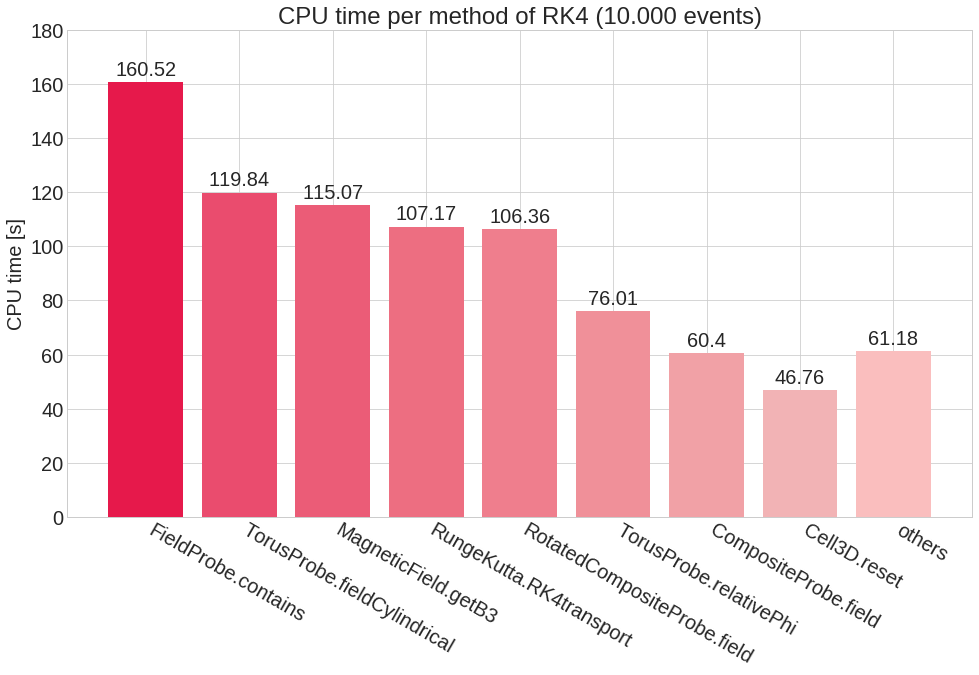
\includegraphics[scale=0.44]{bfield/rk4_composition}
        \caption{\label{fig:rk4_composition} CPU times consumed by each Runge Kutta 4 component.}
    \end{figure}

As seen in Figure \ref{fig:rk4_composition}, most of the Runge Kutta 4 algorithm's runtime is actually used by methods retrieving the magnetic field from the \texttt{swimmer} package.
These methods' purposes is to compute the magnetic field $\textbf{B}(x,y,z) = \langle \operatorname{B_1}(x,y,z),\operatorname{B_2}(x,y,z),\operatorname{B_3}(x,y,z)\rangle$ at a specific $(x,y,z)$ point inside the CLAS12 detector, which is done by placing virtual ``probes'' inside it. % Note: Maybe I should elaborate more on this.

To accelerate this computation, the possibility of using trilinear interpolation~\cite{bourke1999interpolation} for $\mathbf{B}$ was analyzed.
The option was considered favorable since the imprecision brought by interpolating the value instead of directly computing it could be diminished by the \textbf{update} part of the KF and by only using the interpolated magnetic field in a fixed number of iterations of the KF before using the real magnetic field for the remaining ones.
Appendix \ref{add:trilinear_interpolation} describes how trilinear interpolation works.

The algorithm used is a direct transcription of the definition of trilinear interpolation, and is defined in two steps.
First, obtain the regular grid and the measurements at each border, which is done by selecting a grid size $\left([\text{min}_x, \text{max}_x], [\text{min}_y, \text{max}_y], [\text{min}_z, \text{max}_z]\right)$ from which the magnetic field measurements are taken with step sizes defined as $\{\text{ss}_x, \text{ss}_y, \text{ss}_z\}$.
These parameters define a regular tridimensional grid and a measurement for the magnetic field for each point in this grid is obtained.

For the second step, the specific measurement in the location desired is obtained by evaluating the formula defined in \ref{add:trilinear_interpolation}.
In the case that the location is outside the range of the regular grid, the real magnetic field is computed for that point.

After the interpolation algorithm was implemented, the borders and the step size of the grid were left as parameters to be tuned.
First, $[\text{min}_z, \text{max}_z]$ were set to $[229 \text{cm}, 569 \text{cm}]$ since these are the limits of the $z$ variable in the detector.

    \begin{figure}[ht]
        \centering
        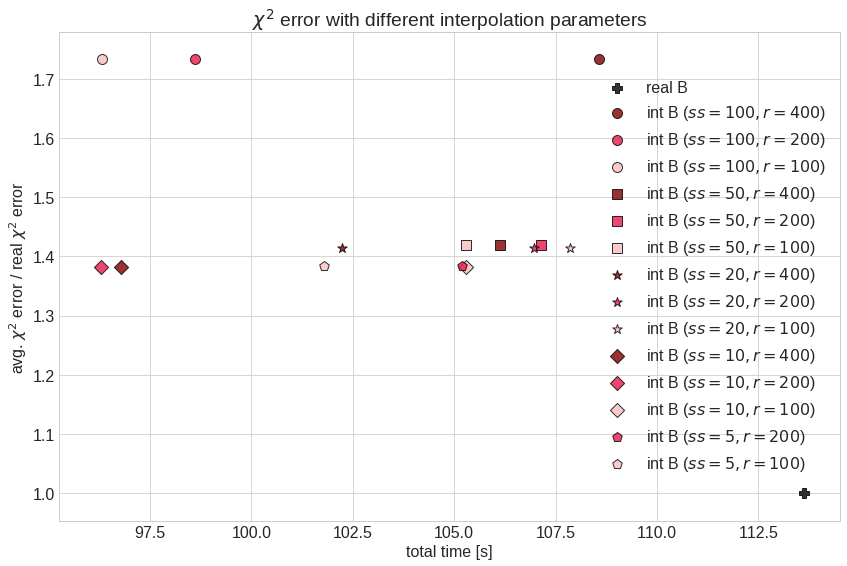
\includegraphics[scale=0.52]{bfield/chi2_vs_time}
        \caption{\label{fig:bfield_chi2_vs_time} $\chi^2$ error when doing the track fitting with the interpolated magnetic field divided by the obtained when using the real magnetic field vs required time. ``real B'' is the real magnetic field while ``int B'' is the interpolated magnetic field with its parameters in parentheses.}
    \end{figure}

To set the step size for each variable, $\text{ss}$ is defined such that $\text{ss} = \text{ss}_x = \text{ss}_y = \text{ss}_z$ for simplicity.
Then, the range $[\text{min}, \text{max}]$ and the variable $r$ are defined such that $\text{min} = \text{min}_x = \text{min}_y$ and $\text{max} = \text{max}_x = \text{max}_y$ and $r = \text{max} = \text{-min}$, to take advantage of the symmetries of the detector, which can be seen in Figures \ref{fig:dc_horizontal_cut} and \ref{fig:dc_vertical_cut} from Section \ref{ssec:framework_dc}.

Tests are ran by running the software using the interpolated magnetic field with different combinations of parameters, comparing them using the division of the $\chi^2$ error obtained by the one found when running the real field and measuring it against the time it takes to run the program.
The results are averaged over a set of $2.500$ estimated tracks and the results can be seen in Figure \ref{fig:bfield_chi2_vs_time}.
It is worth noting that some outliers are removed from the figure to aid with visualization.
The tested values for each were the following:
    \begin{align*}
        \text{ss} &\in \{5 \text{cm}, 10 \text{cm}, 20 \text{cm}, 50 \text{cm}, 100 \text{cm}, 200 \text{cm}\}\\
        r &\in \{100 \text{cm}, 200 \text{cm}, 400 \text{cm}\}
    \end{align*}

As seen in the figure, the interpolation parameters that provide the best results are $\text{ss} = 10 \text{cm}$ and $r = 200 \text{cm}$.

    \begin{figure}[ht]
        \begin{floatrow}
            \ffigbox[0.48\textwidth]{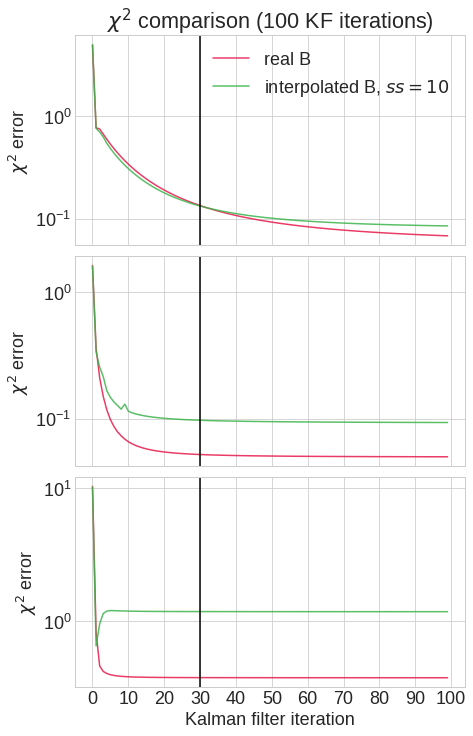
\includegraphics[height=0.72\textwidth] 
            {bfield/chi2_real_vs_ss10}}
                {\caption{\label{fig:bfield_real_vs_ss10} $\chi^2$ error comparison between real magnetic field and interpolated one with a step size of $10$ running the KF with $100$ iterations. A vertical black line denotes the $30$ usual KF iterations.}}
                
            \ffigbox[0.48\textwidth]{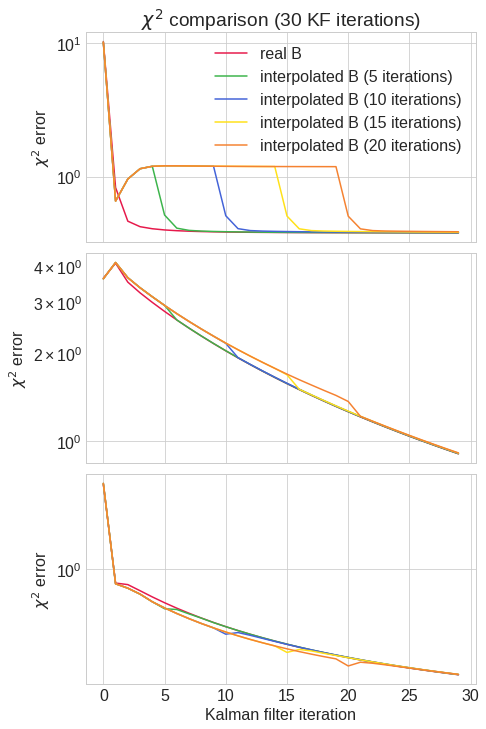
\includegraphics[height=0.72\textwidth] {bfield/chi2_real_vs_ni20}}
                {\caption{\label{fig:bfield_real_vs_ni20} $\chi^2$ error comparison between the real magnetic field and the interpolated one for different numbers of iterations running the KF with $30$ iterations.}}
        \end{floatrow}
    \end{figure}

Figure \ref{fig:bfield_real_vs_ss10} then shows the $\chi^2$ error of three distinct tracks running $100$ KF iterations, contrasting the error of the real magnetic field to that of the selected interpolated version.
As can be seen the figure, in most cases both version converge similarly but the one using the real magnetic field provides better results, albeit generally taking up more time.

Finally, a compromise that still provides good results is reached by running only the first KF iterations using the interpolated magnetic field and the last ones using the real one.
The number of iterations using the interpolated field tested are $0$, $5$, $10$, $15$, $20$, $25$ and $30$, but at the end all but the last one end up with the same final $\chi^2$ error.
Due to this, the number of interpolated magnetic field steps is decided based on the total DCHB and DCTB times when using each version, as presented in Table \ref{tab:interpolated_steps_times}.

It is worth noting that the total times per event listed here are slightly different than the ones presented in the validations of the method, and this is because these tests were ran on $3.000$ events instead of the usual $10.000$.
This decision is taken for the sake of expediency and because it shouldn't affect the results in a significant manner.

    \begin{table}[ht]
        \centering
        \begin{tabular}{@{}l|ll@{}}
        \toprule
        Name                  & DCHB time [s] & DCTB time [s] \\ \midrule
        Real magnetic field   & 130.42        & 48.78         \\
        5 interpolated steps  & 133.42        & 52.05         \\
        10 interpolated steps & 110.94        & 42.24         \\
        15 interpolated steps & 107.87        & 40.76         \\
        20 interpolated steps & 103.83        & 38.46         \\
        25 interpolated steps & 109.52        & 40.14         \\
        30 interpolated steps &  96.63        & 35.14         \\ \bottomrule
        \end{tabular}
        \caption{\label{tab:interpolated_steps_times} DCHB and DCTB times [s] using different interpolated steps.}
    \end{table}

As can be seen in Table \ref{tab:interpolated_steps_times}, the best times were obtained by running $30$ interpolated steps, but the final number of interpolated steps set in the code are $20$, the second best.
This decision is taken due to the fact that, as can be seen in Figure \ref{fig:bfield_real_vs_ni20}, if no steps are taken with the real magnetic field, the final $\chi^2$ error is much higher than the original one.
Figure \ref{fig:bfield_real_vs_ni20} shows the $\chi^2$ error obtained by using this method.

It's worth noting that the interpolation is only implemented in the Hit-Based tracking part of the KF since the Time-Based part requires as much precision as possible.
% Note: This could use a citation but it came from a meeting with Veronique. It's due to the fact that DCTB analyzes using a much finer grain than DCHB, and DCHB is mostly used to quickly filter tracks so that DCTB doesn't need to analyze all of them.
% \newpage
\subsection{Multithreaded Cluster and Track Finding Algorithms} \label{ssec:prop_multithreaded_ctf}
A multithreaded algorithm is an algorithm that takes advantage of the fact that most modern CPUs have more than one core, thus allowing them to concurrently run various execution threads on these multiple cores in order to take less time processing the same data. % Note: Maybe I should cite a book on this.
This is especially useful in the context that the CLAS12 software is ran at JLab, where many data events are computed concurrently, in different machines.
To understand why a multithreaded approach is useful, a bit of insight is needed on how the work in the CLAS12 execution hardware is distributed:

First, a number of threads per engine $T$ is defined in the CLARA configuration file, allowing for $T$ instances of the same engine to process different data events in the different cores at the same time.
Then, if the number of engines running in the production chain is $E$, at most a number of $T\cdot E$ threads will be running at the same time in the HPC cluster.
Dubbing the number of cores at the cluster $C$, a well-tuned configuration file is set so that $T\cdot E \approx C$ so as to utilize the cluster's capacity as best as possible.

Ideally, this setup would work in such a way that all the $C$ cores remain constantly running, but a problem arises due to the fact that the CLAS12 engines require to run in a sequential manner and, as seen in Figure \ref{fig:engines-times-sep2018} from Section \ref{ssec:prob_the_problem}, each engine takes a vastly different amount of time to run.
Because of this, the cores running the faster engines will be left waiting for the slower ones that come previous to them to finish their execution.

Based on this reasoning, a valid approach for accelerating the software is to distribute the work done in the slowest engines, DCHB and DCTB, onto more threads so that the computing time is improved and a better use of the available hardware is ensured.
Two methods for taking advantage of this idea are proposed: A multithreaded algorithm to use in cluster finding and one to use in track finding.

\textbf{Multithreaded Cluster Finding Algorithm}: Analyzing the cluster finding algorithm described in Section \ref{ssec:framework_cf}, it can be seen that there is no reason to do the \textbf{Clump Finding} step before the \textbf{Hit Prunning} one, considering that the second iterates through the hits on a layer-by-layer basis instead of based on the clumps found by the first.

Then, the \textbf{Out-of-Timers Removal}, the \textbf{Cluster Fitting} and the \textbf{Cluster Splitting} steps can be ran in parallel by assigning a thread to each clump found.
It is in theory possible to further parallelize the algorithm by assigning individual threads to each cluster found in the Cluster Splitting step and running the fitting done to them separately, but the estimated gain in computing time is very small due to the fact that only one fit is done on the split clusters, so the option was discarded.

\textbf{Multithreaded Track Finding Algorithm}: The track finding done in the DC code described in Section \ref{ssec:framework_tf} requires a set of measurements to run, which are taken from the hits in six different clusters.
Due to the geometry of the DC detector (which can be seen in Figure \ref{fig:dc_horizontal_cut} from Section \ref{ssec:prob_context}), finding pairs of clusters (dubbed crosses) in the two superlayers that conform a sector is trivial.

Then, all the combinations of three crosses that could potentially make sense as being formed by a particle's trajectory are considered different, independent tracks.
Via the Kalman filter, a fit is attempted for each of these tracks to find the ones that are most likely to be formed by an actual particle passing through the detector.
Considering that each track is fit separately and that they are independent from each other, a multithreaded algorithm is implemented where all the tracks in a data event are fit concurrently in different threads.
% \newpage
% \subsection{Fourth Order Adams-Bashforth-Moulton Method Proof of Concept} \label{ssec:prop_abm}
% Explain why it's a good idea, the separation between two regions and the amount of measurements with a regular step size that can be taken.
As can be seen in figure \ref{fig:dc_horizontal_cut} from subsection \ref{ssec:framework_dc}, the measurements can be divided in the three regions due to the geometry of the detector.
While most of the distances between measurements are usually at most $4$ or $5$ [cm], the distance between regions can be more than a meter.
Also, due to the way that the Kalman Filter works, after transporting the state vector from the first measurement site to the last, this vector needs to be transported back to run the KF again, which requires it to be moved for around $3.5$ meters.

Currently, this movement of the state vector is done through Runge Kutta 4, as is described in subsection \ref{ssec:framework_dc} with a step size $h=1$ so that the $z$ variable is updated by one centimeter in each RK4's iteration, occasionally updating it by $2$ [cm] when the magnetic field at that point is small enough.
Considering that for most particles the majority of the movement from regions $1$ to $2$, $2$ to $3$ and from $3$ back to $1$ the step size is kept at $1$ [cm], the option of changing RK4 for the Fourth order Adams-Bashforth-Moulton (ABM4) method is evaluated.

% Quickly explain the method itself and reference the addendum where it's explained in more detail.
ABM4 is a multi-step method used to solve initial value problems described in detail in \ref{add:abm4}.
The method can solve the same kind of problems as RK4, but it has the advantage that it only requires to evaluate the $\mathbf{f}(z,\mathbf{x})$ function once per iteration, whereas RK4 does this four times.

% Explain a little bit the implementation itself, how RK4 must be used 3 times at the beginning and one time by the end.
The change does not come without disadvantage however, since it requires the use of four previous steps to compute the next one as can be seen in equations \eqref{eq:abm4_explicit} and \eqref{eq:abm4_implicit} from the referenced addendum.
Due to this the step size must be kept constant through each step.
A common and simple-to-execute solution for this is to run RK4 for three steps after the initial state vector, and thus this option is implemented.
It's worth noting that due to the particular conditions of the problem, $z_{k+1}$ does not necessarily fulfill the condition that $z{k+1} = z_k + n h$ where $n$ is an arbitrary natural number, so it's usually impossible to reach the next measurement site from the last one using ABM4, but this is easily fixable by using RK4 at the last step of the process.

% TODO: TALK WITH CT AND SEE IF HE AGREES THAT WE SHOULD SCRAP THIS FOR THE TIME BEING AND MAYBE EXPLORE THE OPTION IN THE FUTURE.

% Explain why the algorithm couldn't be implemented; mention the error associated to the lack of magnetic field differentials.
% After the initial analysis is done, ABM4 is integrated into the code instead of RK4 and tests are ran, but the results are not as good as are expected, as can be seen in figure \textbf{TODO}. % TODO: Add a figure showing the huge errors in the state vector.
% This error is attributed to the issue with the implementation of the equations of motion that is expressed in subsection \ref{ssec:framework_tf}, where equations \eqref{eq:tf_dtx_dx}, \eqref{eq:tf_dtx_dy}, \eqref{eq:tf_dty_dx} and \eqref{eq:tf_dty_dy} cannot be implemented correctly because of the fact that the differentials of the magnetic field $\textbf{B}(x,y,z)$ are unknown, which introduces an instability to the method which causes it to converge to different results when compared to RK4. % TODO: If I'm gonna say that the method didn't work I'm gonna need a better explanation into why I think this is true.

% Still, considering that the theory checks up ABM4 can potentially work in contexts such as this for other particle detectors, and it can be a good idea to try and implement the method if additional information about the system is known in the future.
\newpage
\subsection{Multithreaded Kalman Filter Algorithm Proof of Concept} \label{ssec:prop_multithreaded_kf}

    \begin{wrapfigure}{r}{0.51\textwidth}
        \centering
        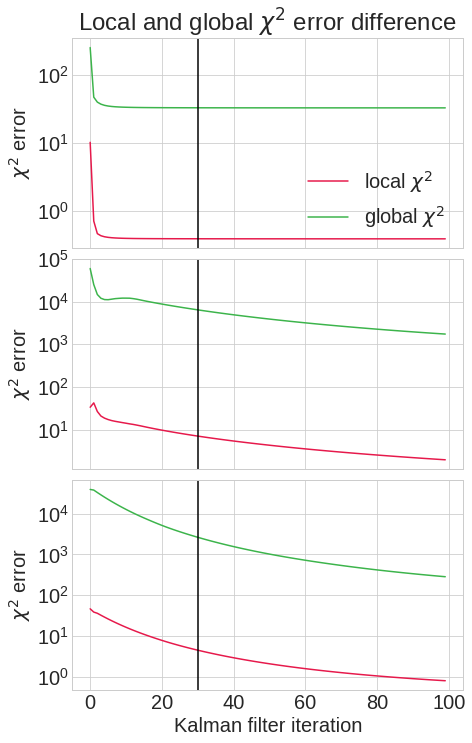
\includegraphics[width=1\textwidth]{multithreaded_kf/chi2error}
        \caption{\label{fig:mkf_chi2error} Local and global $\chi^2$ errors for a track in events \#$5$, \#$67$ and \#$103$ for $100$ KF iterations. The $30$ KF iterations commonly computed are marked by a black vertical line.}
    \end{wrapfigure}

A multithreaded Extended Kalman Filter (EKF) variant is proposed to accelerate the computation of the EKF in the code and to potentially obtain better solutions.
To understand why this option is deemed useful, it has to be noted that the EKF implementation described in Section \ref{ssec:framework_tf} contains a hardcoded stopping point for the EKF after $30$ iterations, with no dynamic analysis onto how good the solution found up to that point is or if the methods used have already converged.
Changing this might open the possibility of a multithreaded algorithm.

% DYNAMIC STOPPING POINT
Due to this, the first efforts were placed on finding this dynamic stopping point for the algorithm.
Naturally, this criteria must be related to the $\chi^2$ error, which is the variable that is being minimized by the method.
As mentioned before, a deifnition of the $\chi^2$ error is given in Appendix \ref{add:errors}.

The problem with this approach is that for every iteration of the EKF only the so-called ``local'' $\chi^2$ error is computed, while the ``global'' one is only computed once the EKF has finished.

% Note: if it's too hard to understand the local and global $\chi^2$ error then it might be better to leave this out for good.
The local $\chi^2$ error is computed while the EKF is running by projecting the state vector at a measurement site into the measurement itself and computing the squared difference divided by the uncertainty of the measurement.
The problem with this version of the error is that as the EKF runs, each state vector changes, and thus the error computed is different from the real one.

The global $\chi^2$ error is this ``real'' one, where each state vector near a measurement site is projected into it and the error is calculated.
The reason that the global error is only computed after the EKF has ran is that the process of updating the state vector across the particle trajectory is computationally-intensive, and thus doing it for each iteration of the EKF would be too expensive for the total computing time.

The problem that arises from this concept is that there are tracks where the convergence of the local $\chi^2$ error is not representative of the converge of the global one.
As can be seen in the first EKF iterations in the track from event \#$67$ in figure \ref{fig:mkf_chi2error}, the local and the global $\chi^2$ errors are not always correlated. % Note: I should find events where this lack of correlation is more apparent.

    \begin{figure}[ht]
        \centering
        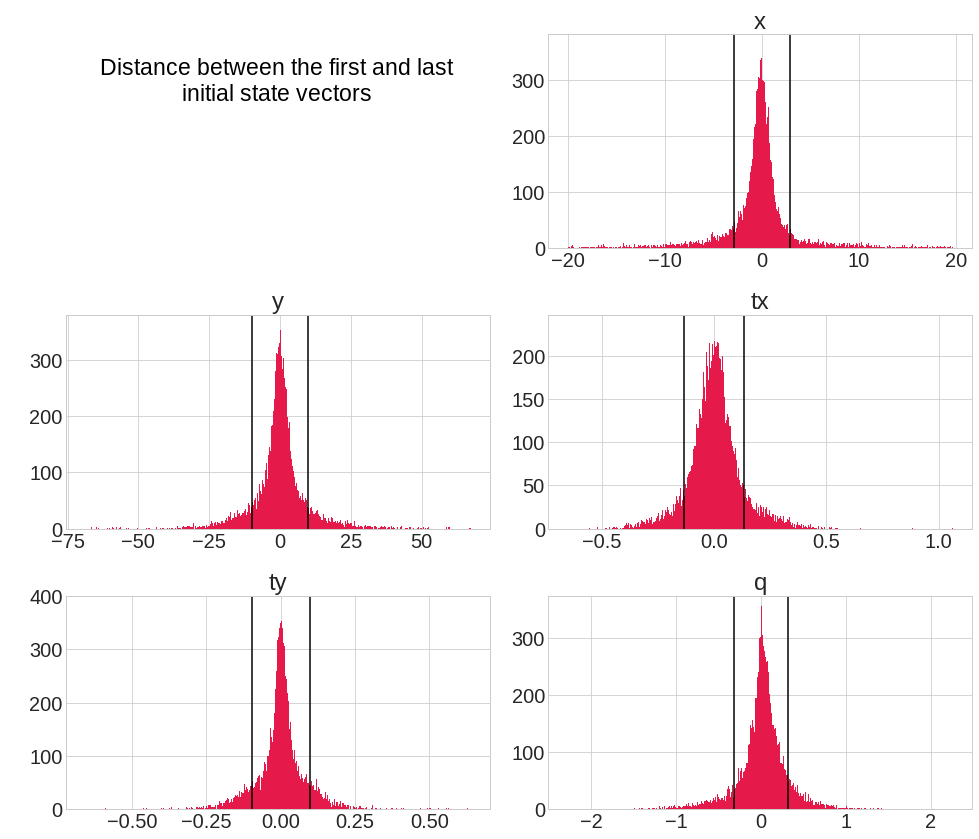
\includegraphics[scale=0.44]{multithreaded_kf/isv_distance}
        \caption{\label{fig:mkf_isv_distance} Distance between the first and the last initial vectors for the tracks found in $10.000$ events. The black lines mark a region where $80\%$ of the distances are contained.}
    \end{figure}

Then, the idea of computing different initial state vectors $\mathbf{x}(z) = \left<x, y, \theta_x, \theta_y, q\right>$ in parallel for each track was considered.
These different initial state vectors should be consistent, and this is pursued by comparing the different variables from the first and the last state vectors used by the Kalman filter.
This difference is recorded for all the tracks found in $10.000$ events and its distribution is evaluated.
A plot of this distribution for each variable in the state vector can be seen in Figure \ref{fig:mkf_isv_distance}.

    \begin{wrapfigure}{r}{0.51\textwidth}
        \centering
        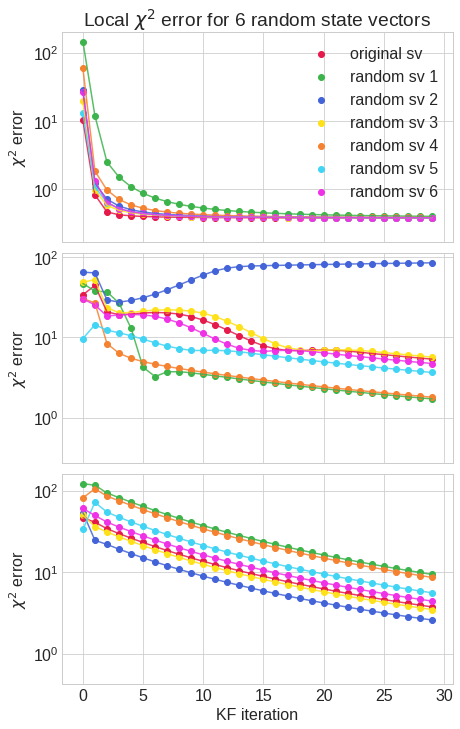
\includegraphics[width=1\textwidth]{multithreaded_kf/mkf_test}
        \caption{\label{fig:mkf_test} Local $\chi^2$ errors starting from $6$ random initial state vectors compared with the original in events \#$5$, \#$67$ and \#$103$ for $30$ KF iterations.}
    \end{wrapfigure}

To generate the initial state vector for the KF to run, a random perturbation inside a range that captures $80\%$ of the distance values (denoted as black vertical lines in Figure \ref{fig:mkf_isv_distance}) is added to the initial state vector and multiple instances of the KF are ran with these different initial state vectors. The resulting $\chi^2$ error obtained by running the KF in this manner for $6$ random initial state vectors can be seen in Figure \ref{fig:mkf_test}.

As can be seen in the figure, for the tracks in events $67$ and $103$ the final $\chi^2$ obtained from a random initial state vector was better than the one obtained for the original.
Special attention should be given to the ones obtained by the random state vectors $1$ and $4$ from event $67$ which are close to a fifth of the original one found.

% INCREASED POWER CONSUMPTION
It's worth noting that if a dynamic stopping point is implemented, that is to say, a point in which the KF is stopped before reaching the $30$ iterations, the multithreaded algorithm may provide better results in the same amount of time as the original one.

It's worth noting that while this algorithm may be able to provide better results in the same amount of time, the approach actually increases the total CPU-time and power consumption required to run the software.
This is due to the fact that multiple instances of the KF run in parallel.
In the case of the CLAS12 software as is ran in JLab, this additional power consumption meant that the algorithm was programmed but not implemented in the code due to power constraints.
    \newpage
    \secnumbersection{SOLUTION VALIDATION} \label{sec:val}

% Note: I could add the validation of each version by mentioning how many tracks are found in each and comparing them with the original tracks found through statistical error.
% Note: Number of tracks found per version by iterating through 10.000 events:
%     v1.0 : 15.575 - 11.248
%     v1.1 : 15.608 - 11.261
%     v1.2 : 15.606 - 11.259
%     v1.3 : 15.606 - 11.257

\subsection{Refactoring and Optimizations} \label{ssec:val_refactoring_and_optimizations}
The changes made described in Section \ref{ssec:refactoring_and_optimizations} brought a CPU time reduction much larger than anticipated, especially for the DCHB engine.
Contrasted to Figure \ref{fig:engines-times-sep2018}, where the time DCHB and DCTB took per event was $169.68$ [ms] and $47.76$ [ms] on average, the new times for each is $118.14$ [ms] and $44.34$ [ms] respectively, meaning an improvement of $30.1\%$ for DCHB and, less impressively, of $7.2\%$ for DCTB.

As shown in Figure \ref{fig:methods_times-1_1}, there are some differences in the percent of the total CPU time distributed on each engine, with a heavy reduction apparent in the \texttt{clusterSplitter} and \texttt{setFitArray} methods.
Using the versioning method mentioned in Section \ref{ssec:prof_results}, this version is named $1.1$.

    \begin{figure}[ht]
        \centering
        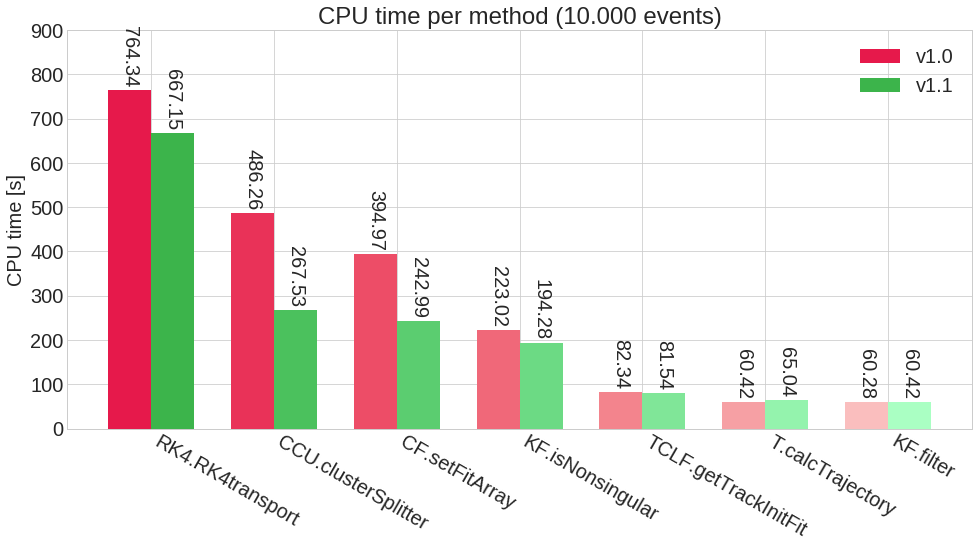
\includegraphics[scale=0.44]{methods_times/1_1}
        \caption{\label{fig:methods_times-1_1} CPU time per method, version $1.1$ contrasted with $1.0$.}
    \end{figure}

A comprehensive list of the improvements is presented:
\begin{itemize}
    \item \textbf{Runge Kutta 4}: The total reduction in the time spent in the \texttt{RK4transport} method was of a $12.7\%$ ($97.19$ seconds) for the $10.000$ events evaluated.
    This is attributed to the precomputation of values achieved via the refactoring of the code that was done after comparing the original code with the real Runge Kutta 4 algorithm.
    Since the original implementation makes very little use of the modularity inherent to the algorithm, the refactoring highlighted that the computations were done repeatedly since the new code is much shorter and easier to comprehend.

    \item \textbf{Cluster Splitter} and \textbf{Set Fit Array}: Both these methods were accelerated in a very similar manner to the one last described, reducing the total CPU time by $45.0\%$ (from $486.26$ to $267.53$ [s]) and by $38.5\%$ (from $394.97$ to $242.99$ [s]) respectively, thus making these two methods less of a priority when compared to RK4.
    
    \item \textbf{Is Nonsingular}: For this method a very small reduction in CPU time is perceived, just of $12.9\%$ (from $223.02$ to $194.28$ [s]) in total.
    No change was made to this method, so the reduction is associated to the addition of better exception handling in previous steps so that iterations with ``useless'' data are stopped before reaching this point in the computation.
    
    \item \textbf{Get Track's Initial Fit}, \textbf{Calculate Trajectory} and \textbf{Filter}: These methods' CPU time were preserved between versions, seeing only very minor change.
    This is attributed to the profiler's measurement error.
\end{itemize}
\subsection{Matrices Handling Changes} \label{ssec:val_matrices}

    \begin{figure}[ht]
        \centering
        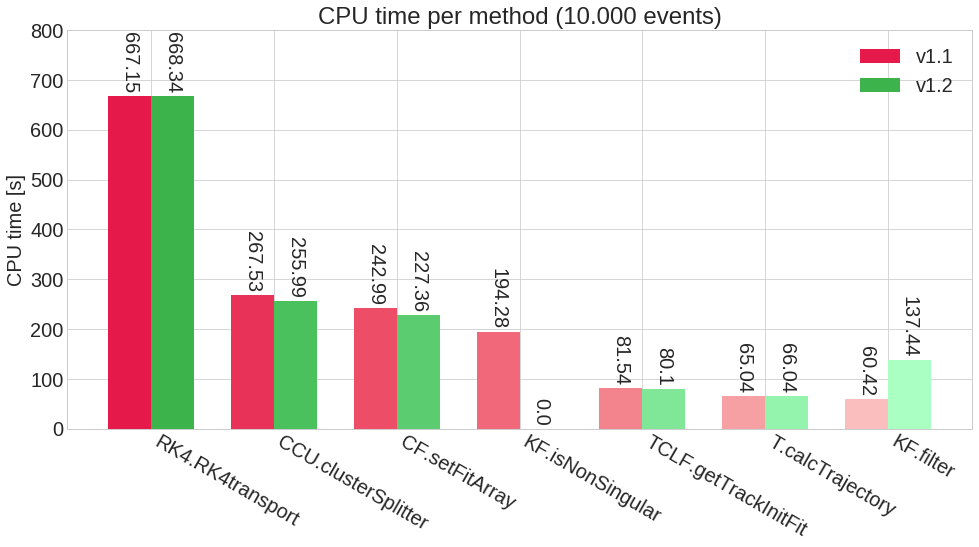
\includegraphics[scale=0.44]{methods_times/1_2}
        \caption{\label{fig:methods_times-1_2} Method CPU times, version $1.2$ compared with $1.1$.}
    \end{figure}

The changes described in Section \ref{ssec:prop_matrices} improve the total CPU time per event of DCHB and DCTB by $4.2\%$ (from $118.14$ to $113.19$ [ms]) and by $3.2\%$ (from $44.34$ to $42.93$ [ms]) respectively.
As shown in Figure \ref{fig:methods_times-1_2}, the \texttt{isNonSingular} method sees a reduction down to $0$ [s] while the \texttt{filter} method sees a significant increase of $127.5\%$ ($77.04$ [s]) and the rest of the methods see very little change, which is only attributed to error between measurements.

The increased time in the \texttt{filter} method is attributed to the fact that the time that was taken by the \texttt{isNonSingular} method is transferred to it due to the changes made to the code. % Note: I sincerely have no idea on to how this happened, I'm guessing it's one of those weird java things.
The net gain in time is of $46.0\%$ (from $254.70$ to $137.44$ [s] in total), which isn't great when considering that the total reduction seen in DCHB and DCTB's times is only of $6.36$ [ms] per event.

The contrast between all the work done and the unremarkable change is attributed to the fact that this work is focused on finely optimizing the code and finding the best methods available to solve the problems, which goes against the principles behind the Java HotSpot compiler as it favors simple-to-understand methods and optimizes them while the application is running, neglecting already optimized code~\cite{meloan1999java}.
This is opposite to the normal behaviour of more standard compilers like gcc, which in turn favors well-optimized code. % Note: Perhaps this last statement needs a citation.


\subsection{Magnetic Field Interpolation} \label{ssec:val_magfield}

    \begin{figure}[ht]
        \centering
        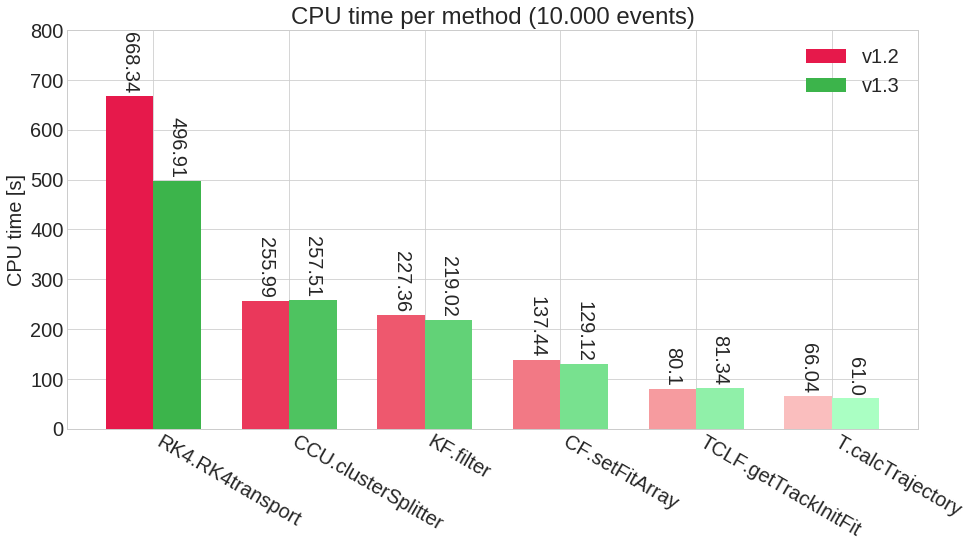
\includegraphics[scale=0.44]{methods_times/1_3}
        \caption{\label{fig:methods_times-1_3} Method CPU times, version $1.3$ compared with $1.2$.}
    \end{figure}
    
The time reduction brought by interpolating the magnetic field described in Section \ref{ssec:prop_magfield} was of $9.2\%$ (from $113.19$ to $102.79$ [ms]) per event for the DCHB engine, while no improvement was seen for DCTB because, as described in the subsection, it isn't considered affordable to lose precision in Time-Based tracking.

Figure \ref{fig:methods_times-1_3} clearly shows that the largest bulk of improvement was in the \texttt{RK4transport} method as should be expected, since this method calls the magnetic field methods that were slowing down the computation.
All the other changes in the different methods are attributed to random differences between the profiling sessions, which are to be expected considering that the profiling was done via statistical sampling, as described in Section \ref{sec:prof}.
\subsection{Multithreaded Cluster and Track Finding Algorithms} \label{ssec:val_multithreaded_ctf}
Considering that the nature of the changes done to the code in this version relate purely to using additional threads to compute results and do not reduce the CPU time, but only the throughput.
It's worth noting that the style of figures that's been used up until now is no longer appropriate, so another is used.

The total time for the DCHB and DCTB engines are compared by running only the multithreaded cluster finding algorithm (version $1.4.\text{a}$), only the multithreaded track finding (version $1.4.\text{b}$), and using both algorithms together (version $1.4$) to get the final total engine time for all the work in this document.
These improvements can be seen in Figure \ref{fig:engines_times-1_4}.

    \begin{figure}[ht]
        \centering
        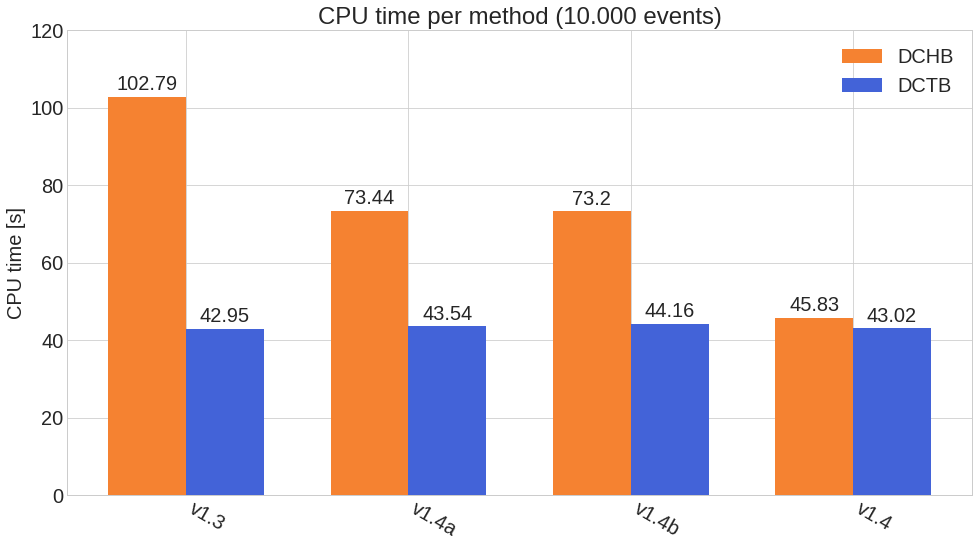
\includegraphics[scale=0.44]{engine_times/mctf_contrast}
        \caption{\label{fig:engines_times-1_4} DCHB and DCTB final CPU times, version $1.4$ compared with $1.3$. Versions $1.4.\text{a}$ and $1.4.\text{b}$ represent only the multithreaded cluster finding and track finding algorithms respectively, while version $1.4$ denotes both together.}
    \end{figure}

\newpage

It's very important to keep in mind that, unlike the other figures, the engine times improvement seen in this figure are not necessarily representative of the actual improvement that will be seen at JLab if and when the changes are implemented.
This is because, as mentioned previously, the hardware used to run the performance tests was a personal computer, and not the cluster where the final implementation will be used.
In its real context, the effectiveness of this version will depend in part on the number of free cores available while running the program, and thus the results obtained will fluctuate depending on this variable.

    \newpage
    \secnumbersection{CONCLUDING REMARKS} \label{sec:concluding_remarks}
The problem faced in this work is multifaceted: it requires to understand the physics behind how particle accelerators and detectors work, then analyze the algorithms to implement these physics in a computer, and finally to code these algorithms in the implementation's environment.
These different facets can also be seen in the contributions of this work.
The team of physicists at JLab see the benefit of a quicker software which allows to analyze the data produced by the detector faster, while the general community benefits from ideas related to particle accelerators, Kalman filters and state estimators in general.

    \begin{figure}[ht]
        \centering
        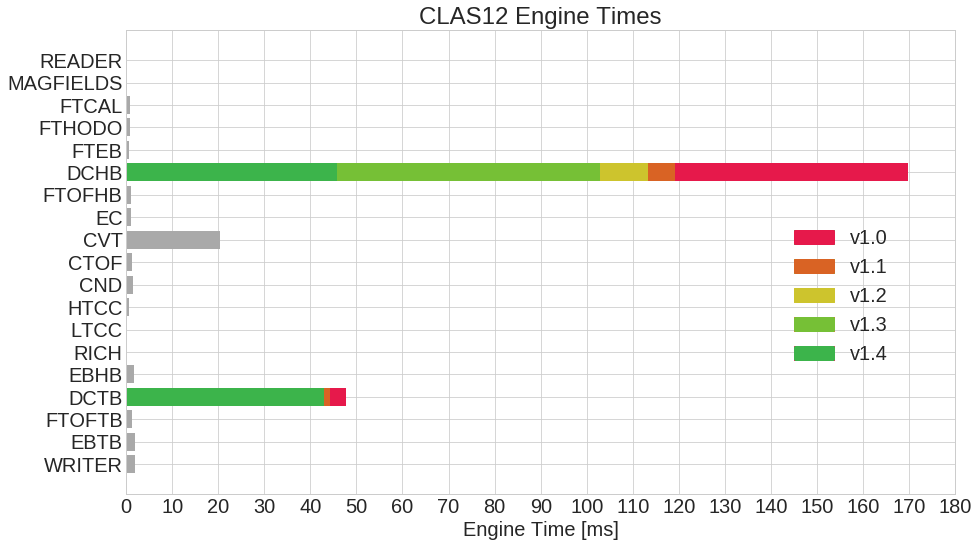
\includegraphics[scale=0.44]{engine_times/1_4}
        \caption{\label{fig:engines_times-final} Engine CPU times.}
    \end{figure}

Regarding the work done for JLab, the improvements on the DCHB and DCTB engines are considerable, as can be seen in Figure \ref{fig:engines_times-final}.
A comprehensive list of each version, it's associated changes to the code, its effect in the total computation time and how useful it is for the community in general follows:
    \begin{itemize}
        \item \textbf{v1.1}: This version consists of the refactoring and optimizations explained in Section \ref{ssec:refactoring_and_optimizations}.
        It's surprising to see that this version brings the largest improvement in computing time, considering that the changes done only apply to the quality of the coding itself and were not changes to the algorithms themselves.

        This odd behaviour is explained by two main reasons: First, the changes reduce a large amount of unnecessary computations.
        Second and more importantly, the fact that the code was simplified allowed the Java HotSpot Performance Engine to apply heavier dynamic optimizations in runtime to the program~\cite{hunt2011java}.
        
        While this version provides a large improvement for the CLAS12 software, its implementation is mostly only useful for JLab since it is a direct quality improvement of their code and doesn't mean any change for the community in general. % Note: Maybe I should be more detailed when talking about ``the community''?
        
        \item \textbf{v1.2}: This version consists on the implementation of different algorithms to improve the way matrices are handled by the Kalman Filter.
        This change doesn't provide a very significative improvement to the total computing time of CLAS12, which is attributed mostly to the matrix library used in the software, JAMA.
        While the changes brought heavily reduce the complexity of the operations completed in the software as is evidenced in Section \ref{ssec:prop_matrices}, they also require a higher amount of matrices to be initialized, which isn't too efficient in the library~\cite{hicklin2000jama}. % Note: I could add a figure that evidences this. If I look at the matrices computations while profiling it can be seen that around 9% of the total time spent is spent initializing matrices.
        
        However, the changes applied could produce a bigger improvement for other particle detectors' software or for other instances of the EKF, considering that the need for matrix inversions and multiplications is completely eliminated in the Update phase of the filter.
        A potential future work that is proposed to reap the benefit of the work done in this version would be to switch to another matrix library or implement a new one that takes better advantage of these changes.
        
        \item \textbf{v1.3}: This version relates to the implementation of a magnetic field interpolation algorithm as is described in Section \ref{ssec:prop_magfield}.
        Again, this change doesn't provide a very big difference on the final computing time of DCHB, but it has the advantage of producing such improvements with minimal effect on the precision of the results.
        As for the benefit that this work could provide for the community in general, its potential is limited by its use; while other publications provide interpolation methods with much higher accuracy~\cite{mackay2006divergence}, this one provides very quickly computed results which can be accurate enough for certain applications, as can be seen in Figure \ref{fig:bfield_slice}.
        
            \begin{figure}[ht]
                \centering
                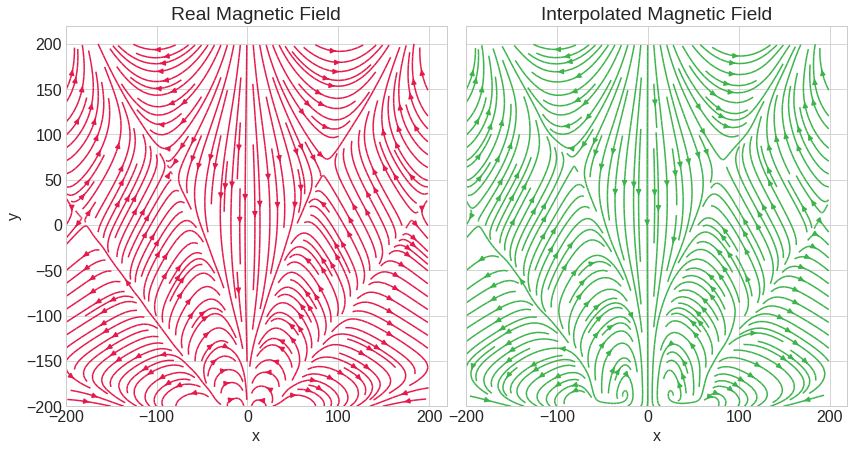
\includegraphics[scale=0.515]{bfield/bfield_slice}
                \caption{\label{fig:bfield_slice} Vertical cut through the magnetic field transverse to the beam line at $z=500$ [cm].}
            \end{figure}

        \item \textbf{v1.4}: This version simply shows an exploitable capability of particle detectors, which is that many hit clustering and particle tracking algorithms that are currently employed for particle detectors work with independent tracks, and thus are easily parallelizable~\cite{blum2008particle}.
        
        \item \textbf{Additional developments}: The work presented in subsection \ref{ssec:prop_multithreaded_kf}, while not implemented in CLAS12 due to specific constraints, provides useful insight into they improvement they could bring to other particle detectors.
        
        \newpage
        
        The alternative of utilizing the multithreaded KF algorithm proposed can potentially find better final tracks found if the additional computing time can be spared.
        Also, if more time is given to fine-tune this algorithm, it has the potential of improving computing time by analyzing different tracks with less KF iterations, thus diversifying the space used for initial state vectors.
    \end{itemize}

% PROPOSED FUTURE WORK
During the development of this project, some ideas were not evaluated or implemented because they fell out of the scope of this work or because they were not useful in the specific case of CLAS12, but may be useful for other particle detectors that employ Drift Chambers.
A list of these is offered with the hope that they will be investigated in future works:

    \begin{itemize}
        \item \textbf{Fourth Order Adams-Bashforth-Moulton method}: As can be seen in Figure \ref{fig:dc_horizontal_cut} from Section \ref{ssec:framework_dc}, the measurements can be divided in three regions due to the geometry of the detector.
        While most of the distances between measurements are usually at most $4$ or $5$ [cm], the distance between regions can be more than a meter.
        Also, due to the way that the Kalman Filter works, after transporting the state vector from the first measurement site to the last, this vector needs to be transported back to run the KF again, which requires it to be moved for around $3.5$ meters, or the entire length from sector $3$ to sector $1$.
    
\newpage

        Currently, this movement of the state vector is done through Runge Kutta 4, as is described in Section \ref{ssec:framework_dc} with a step size $h=1$ so that the $z$ variable is updated by one centimeter in each RK4's iteration, occasionally updating it by $2$ [cm] when the magnetic field at that point is small enough.
        Considering that for most particles the majority of the movement from regions $1$ to $2$, $2$ to $3$ and from $3$ back to $1$ the step size is kept at $1$ [cm], the option of switching RK4 for the Fourth order Adams-Bashforth-Moulton (ABM4) method for these intervals is evaluated.

        ABM4 is a multi-step method used to solve initial value problems described in detail in Appendix \ref{add:abm4}.
        The method can solve the same kind of problems as RK4, but it has the advantage that it only requires to evaluate the $\mathbf{f}(z,\mathbf{x})$ function twice per iteration, whereas RK4 does this four times.

        The change does not come without disadvantage however, since it requires the use of four previous steps to compute the next one as can be seen in equations \eqref{eq:abm4_explicit} and \eqref{eq:abm4_implicit} from the appendix.
        Due to this the step size must be kept constant through each step, and RK4 needs to be ran for three steps after the initial state vector.
        It's worth noting that due to the particular conditions of the problem, $z_{k+1}$ does not necessarily fulfill the condition that $z_{k+1} = z_k + n h$ where $n$ is an arbitrary natural number, so it's usually impossible to reach the next measurement site from the last one using ABM4, but this can be fixed easily by using RK4 between the last step reached by ABM4 and the measurement plane $z_{k+1}$.

        Due to specific difficulties and time constraints this option was programmed but not implemented, but it's considered a valuable option for future work.
    
        \item \textbf{Split cluster filtering}: While working with the software, it was observed that some split clusters separated using the cluster splitting algorithm described in Section \ref{ssec:framework_cf} are actually produced by what looks like one or a few particles and a large amount of noise.
        The split clusters then go through the track finding algorithm described in Section \ref{ssec:framework_tf} normally and a large portion of time is spent fitting each separately to then be scrapped as noise.
        
        This time could potentially be reduced by running a special track finding algorithm that analyzes them with more scrutiny before running the rest of the algorithm.
        Another option would be trying to fine tune the parameters in the cluster splitting algorithm so that, ideally, these noise clusters would be removed before it is attempted to find tracks from them.
    
        \item \textbf{Magnetic field interpolation parameter tuning}: Regarding the magnetic field interpolation proposed in Section \ref{ssec:prop_magfield}, the parameter tuning could use much more work which was not considered due to the large amount of time the tests would take.
        The option of fine tuning each parameter separately opens the possibility of a more precise or faster implementation by offering a smaller step size in some dimensions or different ranges for the $x$ and $y$ variables.
        
        \item \textbf{Alternate magnetic field interpolation methods}: Attention is also brought to the fact that only trilinear interpolation is used.
        Triquadratic or tricubic interpolation might produce more accurate results, but they were not attempted due to the fact that they could potentially be far slower than the original implementation, which would work against the original objective of interpolating the field in the first place.
        
        \item \textbf{Kalman Filter Fine Tuning}: The EKF implemented in CLAS12 works with various parameters, like the number of iterations, the Runge-Kutta 4 original step size and its criteria for increasing this step size, the convergence criteria for stopping the filter before reaching the maximum number of iterations, and the newly introduced number of iterations using the interpolated magnetic field.

        All of these parameters were set somewhat haphazardly, by trial and error.
        The option of running another Kalman Filter that trains the original one by fine-tuning these parameters is proposed, with the alternative of using methods from machine learning, which has already been done in the academy~\cite{abbeel2005discriminative}.
        
        \item \textbf{Hough-Transform-based cluster finding}: An option that was considered but quickly discarded due to time constraints is that of using the Hough Transform (described in Appendix \ref{add:hough_transform}) over the set of all the hits in one event instead of only to split clusters.
        
        While this option would probably be slower in CPU, it offers the possibility of leveraging this computation to a GPU, which has already been proved possible~\cite{braak2011fast}, even for the specific case of particle accelerators, such as the LHC~\cite{halyo2013gpu}.
        
        \item \textbf{FPGA-or-ASIC-based cluster finding}: Another option that was considered but not tried is that of migrating the cluster finding described in Section \ref{ssec:framework_cf} to hardware via Field Programmable Gate Arrays (FPGAs) or Application-Specific Integrated Circuits (ASICs).
        The proposal comes from the fact that the Clump Finding and Hit Pruning parts of the algorithm are very basic and can be done without any floating-point computation, task that famously can be hard for FPGAs~\cite{fagin1994field}.
        
        It might even be possible to run the whole cluster finding algorithm in FPGAs by discovering a good implementation of the \textbf{Cluster Fitting} and \textbf{Cluster Splitting} parts of the algorithm that don't heavily rely on floating-point operations.
    \end{itemize}

Special attention is brought again to the fact that the biggest improvement in the code is seen in version $1.1$, the ``code clean-up''.
The refactoring done was not completely thorough, and perhaps even larger changes can be obtained by reworking the DC software by rewriting most classes from the algorithm up.

\newpage

A final reflection on this same subject relates to the language choice for the CLAS12 software, Java.
In the current programming environment, where processing units' focus is shifting from complex and fast general purpose CPUs to lower-power, multi-core processor units, the software should be adapting alongside the hardware and a shift to languages with small memory footprint and well-defined states should be preferred.
This change of focus can be seen, for example, in the software development for the LHC, where clear guidelines have been stated to switch software to C++~\cite{foundation2017roadmap} and to use simpler date structures, drifting away from the objects common to object-oriented programming~\cite{cerati2016kalman}.

While originally the choice of using Java might have made sense, in the current context of high performance computing this option is disputed.
It has been repeatedly proven that C/C++ provides at least double the computing speed of Java and at most a quarter of the memory usage~\cite{prechelt2000empirical}, with even larger differences found in other studies~\cite{prechelt1999comparing}.
Changing the codebase to C/C++ can even be aided by the computing framework, CLARA, due to the fact that it supports services in both Java and C++~\cite{gyurjyan2013clara}, which means that the change could be applied gradually; thus allowing for incremental tests to be applied while this change is taking place.
    \newpage

    \setcounter{section}{8}
\secnumberlesssection{APPENDICES}
\subsection{On the Flops of Different Operations} \label{add:flops}
Floating point operations per second or flops is a measure for computer performance usually considered more accurate than the instructions per second. % Note: This might need a citation.
It is commonly stated that some operations require more flops than others, so different operations are considered separately when analyzing the computational complexity.
For the study done in this document, different operations are counted together for simplicity and due to the fact that, as can be seen in Table \ref{tab:op_times}, their computation time is not too different in modern architectures, or at least in a personal computer's CPU.

    \begin{table}[h]
        \centering
        \begin{tabular}{@{}ll@{}}
        \toprule
        operation & time {[}ns{]} \\ \midrule
        sum       & $1.7005$   \\
        mul       & $1.4478$   \\
        div       & $1.8587$   \\
        sqrt      & $1.7818$   \\ \bottomrule
        \end{tabular}
        \caption{\label{tab:op_times} Operation times in [ns].}
    \end{table}

Due to a very high variance in the operation time during different iterations of the same code in Java and the language's lack of capacity to do high-precision tests, the tests to obtain these values were performed in C.

The tests were ran by measuring the CPU time in the machine before and after each operation was done on pseudo-random double-precision floating point values using the \texttt{clock()} function from the \texttt{time.h} library.
Each operation was performed $10.000.000$ times and the average computation time was used to minimize statistical error on an Intel(R) Core(TM) i$5$-$6600$K CPU with $4$ cores running at $3.50$GHz with $8$GB of DDR$4$ $2133$MHz RAM.
The source code for this test can be seen in \texttt{https://gist.github.com/bleaktwig/} \texttt{211dab3a5f95b4e857f1f001d7b13654}.
\subsection{Error Measurements} \label{add:errors}
The quadratic error, mean squared error (MSE) or $\chi^2$ error of a procedure estimating a random variable measures the average of the squares of the errors between each measured variable and their estimated value.
With $\hat{y} = f(x)$ being a function of measured values $y$ and $n$ being the number of samples taken such that ${y_1, y_2, ..., y_n}$ are known and ${\hat{y}_1, \hat{y}_2, ..., \hat{y}_n}$ can be obtained from $\hat{y}_i = f(x_i)$, the quadratic error of the function can be defined as~\cite{taylor1997introduction}:
    \begin{equation*}
        \chi^2 = \frac{1}{n} \sum\limits_{i=1}^n \frac{(y_i - \hat{y}_i)^2}{\hat{y}_i}\,.
    \end{equation*}
In the case of the DC software, the quadratic error is used to describe how good a track fit is when compared to the measured data.
\subsection{Covariance Matrix} \label{add:covariance_matrix}
Given a random vector $\mathbf{x}$ of size $n$ defined as $\mathbf{x} = \{x_1, x_2, ..., x_n\}$, the covariance matrix $\Sigma$ of such vector is usually defined as:
    \begin{equation*}
        \Sigma = 
        \begin{bmatrix}
            \text{var}(x_1) & \text{cov}(x_1, x_2) & \dots & \text{cov}(x_1, x_n) \\
            \text{cov}(x_2, x_1) & \text{var}(x_2) & \dots & \text{cov}(x_2, x_n) \\
            \vdots & \vdots & \ddots & \vdots \\
            \text{cov}(x_n, x_1) & \text{cov}(x_n, x_2) & \dots & \text{var}(x_n)
        \end{bmatrix}\,,
    \end{equation*}
with $\text{var}(x_i)$ signifying the variance of the random variable $x_i$ and $\text{cov}(x_i, x_j)$ the covariance of variables $x_i$ and $x_j$.
Variances and covariances are defined as:
    \begin{align*}
        \text{var}(x) &= \frac{1}{m}\,\sum\limits_{i=1}^m (x_i - \bar{x})^2\\
        \text{cov}(x,y) &= \frac{1}{m-1}\,\sum\limits_{i=1}^m (x_i - \bar{x})(y_i - \bar{y})\,,
    \end{align*}
where $\bar{x}$ denotes the mean or average of $x$, and is defined as:
    \begin{equation*}
        \bar{x} = \frac{1}{m}\,\sum\limits_{i=1}^m x_i\,,
    \end{equation*}
where $m$ denotes the number of measurements.

Due to the fact that by definition neither variances or covariances can be negative and that $\text{cov}(x_i, x_j) = \text{cov}(x_j, x_i)$, the covariance matrix $\Sigma$ of a vector is always symmetric and positive-definite.
\newpage
\subsection{Jacobian Matrix} \label{add:jacobian_matrix}
For an arbitrary vectorial function $\mathbf{f}(\mathbf{x})$, the jacobian matrix is a matrix that lists all its first-order partial derivatives.
Assuming that the function $\mathbf{f}(\mathbf{x})$ can receive a generic input vector $\mathbf{x} = \{x_1, x_2, ..., x_n\} \in \mathbb{R}^n$ and produces an output $\mathbf{f}(\mathbf{x}) = \{f_1(\mathbf{x}), f_2(\mathbf{x}), ..., f_m(\mathbf{x})\} \in \mathbb{R}^m$, then the Jacobian matrix $J_f$ of $\mathbf{f}(\mathbf{x})$ is the $m\times n$ matrix defined in the following manner:
    \begin{equation*}
        J_f = 
        \begin{bmatrix}
            \frac{\partial f_1}{\partial x_1} & \frac{\partial f_1}{\partial x_2} & \dots & \frac{\partial f_1}{\partial x_n} \\[6pt]
            \frac{\partial f_2}{\partial x_1} & \frac{\partial f_2}{\partial x_2} & \dots & \frac{\partial f_2}{\partial x_n} \\[6pt]
            \vdots & \vdots & \ddots & \vdots \\[6pt]
            \frac{\partial f_m}{\partial x_1} & \frac{\partial f_m}{\partial x_2} & \dots & \frac{\partial f_m}{\partial x_n}
        \end{bmatrix}\,.
    \end{equation*}
\subsection{Hough Transform} \label{add:hough_transform}

    \begin{wrapfigure}{r}{0.45\textwidth}
        \centering
        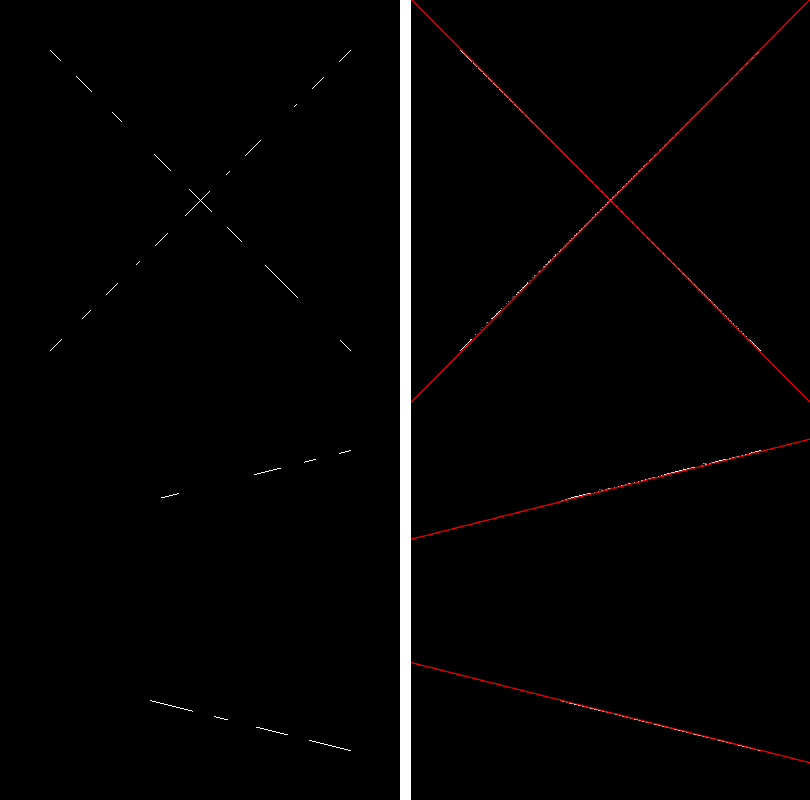
\includegraphics[width=1\textwidth]{hough_transform}
        \caption{\label{fig:hough_transform} Hough transform example. The red lines on the right image denote the lines found by the method.}
    \end{wrapfigure}

The Hough Transform is a method usually utilized to extract features in image analysis, originally proposed by Paul Hough~\cite{hough1962method}.
The method is used to detect simple shapes such as straight lines or circles in any set of points with given coordinates (usually from images) by finding groupings in these sets via a voting procedure over a set of parameterized properties.
An example of the detection of straight lines can be seen in Figure \ref{fig:hough_transform}.
In the left image the points are marked in white, while in the right image the lines found are marked in red.

For the case of detecting straight lines in two dimensions, the line is defined as $y = mx + b$ with its representation in its \textbf{Hessian normal form}~\cite{gellert2012vnr} is:
    \begin{equation*}
        r = x\cos{\theta} + y\sin{\theta}\,,
    \end{equation*}
where $r$ is the distance from the origin to the closest point in the line and $\theta$ is the angle between the $x$ axis and the line.
Given a point in the plane, the set of all lines going through that point corresponds to a sinusoidal curve in the $(r,\theta)$ plane.
A set of more than one point that form a straight line will produce multiple sinusoids crossing at the $(r,\theta)$ plane for that line, and thus, the original problem of detecting collinear points can be expressed as the problem of finding concurrent curves.
\subsection{Architectural Technical Debt} \label{add:technical_debt}
The term ``Technical Debt'' is attributed to a concept described as a debt that arises when ``shipping first time code''~\cite{cunningham1992wycash}.
This is a debt in the sense that the code written works correctly but will eventually require the programmer to use time to re-write it with the added knowledge of how it will interact with the rest of the code.
The term becomes significant when the programmer doesn't spend the time required to fix the code and continues working on the code base, causing the debt to accumulate ``interest'', so that when the issue is finally addressed it is much harder to do so due to all the code that works interconnected to this ``dirty'' code.

Technical debt can be intentional or unintentional, and managed or unmanaged.
An intentional debt refers to one incurred by a programmer who is aware of the future time it will take to fix the code, while an unintentional one to one incurred by accident due to either lack of knowledge about the ``engineering best practices'', not applying the correct abstractions, writing a simple but slow algorithm, among others.
A managed debt refers to one where the programmer is aware of the debt and plans to fix it before creating new components dependant on the code where the debt is owed, while an unmanaged debt refers to the contrary~\cite{allman2012managing}.

It is evident that an unintentional, unmanaged debt causes long term instability issues with a program, while an intentional and managed debt can be used as a tool by the programmer to provide quick fixes or releases, but taking the time later to repay the debt.
The two other possible cases are more rare; an intentional, unmanaged debt either means that the programmer is in a hurry or he/she simply doesn't care.
An unintentional managed debt is even more unlikely~\cite{allman2012managing} and may be simply described as a happy accident.
\subsection{Sherman-Morrison Formula} \label{add:shermanmorrison_formula}
Originally proposed by Jack Sherman and Winifred J. Morrison~\cite{sherman1950adjustment}, the Sherman-Morrison formula says that if $A\in\mathbb{R}^{n\times n}$ is a nonsingular matrix and $\mathbf{u}, \mathbf{v} \in\mathbb{R}^n$ are vectors:
    \begin{equation*}
        (A + \mathbf{u}\mathbf{v}^T) = A^{-1} - \frac{A^{-1}\mathbf{u}\mathbf{v}^T A^{-1}}{1 + \mathbf{v}^T A^{-1} \mathbf{u}}\,,
    \end{equation*}
given that $1 + \mathbf{v}^T A^{-1} \mathbf{u} \neq 0$.

\newpage

This formula is especially useful when $A^{-1}$ is unknown but $A$ is known, or in special cases such as the one seen in Equation \eqref{eq:mhc_sm_det}, where:
    \begin{align*}
        P_{k|k} &= (P_{k|k-1}^{-1} + \mathbf{h}\mathbf{h}^T)^{-1}\\
        &= P_{k|k-1} - \frac{P_{k|k-1} \mathbf{h} \mathbf{h}^T P_{k|k-1}} {1 + \mathbf{h}^T P_{k|k-1} \mathbf{h}}\,,
    \end{align*}
since it eliminates the need to compute the inverse of $P_{k|k-1}$ and, if the operations are resolved in a particular order, it even eliminates the need for multiplying matrices, which is an expensive operation by itself. 
% Note: If I add an addendum "On the complexity of operating matrices" this should ref there.
% \newpage
\subsection{Su-Chang Formula} \label{add:suchang_formula}
Originally proposed by Ching Tzong-Su and Feng Cheng Chang~\cite{su1996quick}, the Su-Chang formula proposed a method to compute the determinant of a square matrix $A$ by splitting it into a matrix $W\in\mathbb{R}^{(n-1)\times(n-1)}$, two column vectors $\mathbf{u}\in\mathbb{R}^{n-1}$ and $\mathbf{v}\in\mathbb{R}^{n-1}$ and a scalar $r\in\mathbb{R}$:
    \begin{align*}
        |A| &=
        \begin{vmatrix}
            W            & \mathbf{v} \\
            \mathbf{u}^T & r
        \end{vmatrix}\\
        &= r\cdot\Big|W - \frac{\mathbf{v}\mathbf{u}^T}{r}\Big|\,,
    \end{align*}
given that $r\neq0$.

A recursive algorithm can then be defined as:

    \begin{algorithm}[H]
        \caption{Su-Chang algorithm}
        \label{alg:suchang}
        \SetAlgoLined
        \DontPrintSemicolon
        \SetKwProg{Def}{def}{:}{}
        \Def{\upshape suchang\_det($A$: matrix, $n$: int)}{
            \uIf{\upshape $n$ == $1$}{
                \Return $a_{00}$\;
            }
            $W = 
            \begin{bmatrix}
                a_{0,0}     & a_{0,1}     & \dots  & a_{0,(n-1)}\\
                a_{1,0}     & a_{1,1}     & \dots  & a_{1,(n-1)}\\
                \vdots      & \vdots      & \ddots & \vdots\\
                a_{(n-1),0} & a_{(n-1),1} & \dots  & a_{(n-1),(n-1)}\\
            \end{bmatrix}$\;
            $\mathbf{v} = \left< a_{0,n}, a_{1,n}, \dots, a_{(n-1),n} \right>$\;
            $\mathbf{u} = \left< a_{n,0}, a_{n,1}, \dots, a_{n,(n-1)} \right>$\;
            $r = a_{n,n}$\;
            \Return $r \cdot$ suchang\_det\big($W - \frac{\mathbf{v}\mathbf{u}^T}{r}$\big)\;
        }
    \end{algorithm}

where $n$ is the square matrix $A$'s row and column dimension.

% From this, the algorithm's complexity can be obtained:
%
%     \begin{align*}
%         &\mathbf{v}\mathbf{u}^T &\rightarrow (n-i)\\
%         &\frac{\mathbf{v}\mathbf{u}^T}{r} &\rightarrow (n-i) + 1\\
%         &W - \frac{\mathbf{v}\mathbf{u}^T}{r} &\rightarrow (n-i)^2 + (n-i) + 1\\
%         &\Big|W - \frac{\mathbf{v}\mathbf{u}^T}{r}\Big| &\rightarrow \sum_{i=1}^{n-2} (n-i)^2 + (n-i) + 1\\
%         &r\cdot\Big|W - \frac{\mathbf{v}\mathbf{u}^T}{r}\Big| &\rightarrow \sum_{i=1}^{n-2} (n-i)^2 + (n-i) + 2
%     \end{align*}

If each step of the algorithm is denoted by $i$, it's easy to see that each step requires $(n-i)^2 + 1$ multiplications, $(n-i)^2$ subtractions and $1$ division.
From this, the mathematical complexity can be calculated:

    \begingroup
    \allowdisplaybreaks
    \begin{align}
        \text{C}(\text{suchang\_det}(A)) &= \sum_{i=1}^{n-2} ((n-i)^2 + 1 + (n-i)^2 + 1)\nonumber\\
        &= 2\sum_{i=1}^{n-2} ((n-i)^2 + 1)\nonumber\\
        &= 2\sum_{i=2}^{n-1} (i^2 + 1)\nonumber\\
        &= \frac{1}{3}(2n^3 - 3n^2 + 7n - 18)\,,\label{eq:suchang_complexity}
    \end{align}
    \endgroup
    
which is much less than the $n^3 + \mathcal{O}(n^2)$ usually required to compute a matrix's determinant through LU decomposition~\cite{banachiewicz1937berechnung}.

It's worth noting that other publications extend this algorithm, but only address the problem that arises when a component of the $A$ matrix's diagonal is $0$, and don't improve further its efficiency~\cite{chang1998more,chang2014determinant}.
\subsection{Cholesky Matrix Decomposition} \label{add:cholesky_decomp}
If $A\in\mathbb{R}^{n\times n}$ is a symmetric positive-definite matrix, there exists a lower diagonal matrix $L\in\mathbb{R}^{n\times n}$ such that:
    \begin{equation*}
        A = L\,L^T\,.
    \end{equation*}

Algorithmically, a na\"ive implementation for each component of $L$ is shown in algorithm \ref{alg:chol_decomp}.
    \begin{algorithm}
        \caption{Cholesky Decomposition}
        \label{alg:chol_decomp}
        \SetAlgoLined
        \DontPrintSemicolon
        \SetKwProg{Def}{def}{:}{}
        \Def{\upshape cholesky\_decomposition($A$: matrix, $n$: int)}{
            $l_{1,1} = \sqrt{a_{1,1}}$\;
            \For{$j\gets2$ \KwTo $n$}{
                $l_{j,1} = \frac{a_{j,1}}{l_{1,1}}$\;
            }
            \For{$i\gets2$ \KwTo $n$}{
                $l_{i,i} = \sqrt{a_{i,i} - \sum\limits_{p=1}^{i-1} l_{i,p}^2}$\;
                \uIf{$i \neq n$}{
                    \For{$j\gets i+1$ \KwTo $n$}{
                        $l_{j,i} = \frac{1}{l_{i,i}}\left(a_{j,i} - \sum\limits_{p=1}^{i-1} l_{i,p}\cdot l_{j,p}\right)$\;
                    }
                }
            }
        }
    \end{algorithm}

From the algorithm, it can be seen that the decomposition requires the calculation of $n$ square roots, $\frac{1}{2}n(n-1)$ divisions, $\frac{1}{6}n(n^2 - 1)$ multiplications, $\frac{1}{6}n(n^2 - 3n - 4)$ additions and $\frac{1}{2}n(n + 1)$ subtractions.
Summed together, these add up to a total of $\frac{1}{6}n(2n^2 + 3n + 1)$ operations.
\newpage
\subsection{Matrix Determinant Lemma} \label{add:mat_det_lemma}
The matrix determinant lemma can be defined as follows~\cite{brookes1998matrix}:
    \begin{lemma}
        If $A\in\mathbb{R}^{n\times n}$ is an invertible square matrix and $\mathbf{u}, \mathbf{v} \in\mathbb{R}^n$ are column vectors, it can be proven that:
            \begin{equation*}
                |A + \mathbf{u}\mathbf{v}^T| = (1 + \mathbf{v}^T A^{-1} \mathbf{u}) \cdot |A|\,.
            \end{equation*}
    \end{lemma}

The lemma is especially useful in cases where $|A|$ and $A^{-1}$ are already known, since it allows for the calculation of the determinant of $A$ updated by adding the matrix $\mathbf{u}\mathbf{v}^T$ to it without computing the new determinant from scratch.
\subsection{Cauchy-Schwarz Inequality} \label{add:cauchy_schwarz}
The Cauchy-Schwarz inequality or Cauchy-Bunyakovsky-Schwarz inequality is a very useful inequality which states that, if $\mathbf{u}$ and $\mathbf{v}$ are any vectors inside an inner product space, it can be proven that:
    \begin{equation*}
        |\langle \mathbf{u}, \mathbf{v} \rangle| \leq \|\mathbf{u}\|\|\mathbf{v}\|\,,
    \end{equation*}
where $\langle \cdot,\cdot \rangle$ is the inner product~\cite{strang2005linear}.

Considering that the expectation of a product of two random variables is an inner product, this leads to the covariance inequality:
    \begin{equation*}
        |\text{cov}(x,y)|^2 \leq \text{var}(x)\text{var}(y)\,,
    \end{equation*}
where $\text{var}(\cdot)$ denotes the variance of a variable and $\text{cov}(\cdot,\cdot)$ the covariance between two, and are defined in Appendix \ref{add:covariance_matrix}.
% \subsection{On the Computation of Matrix Operations} \label{add:matrix_complexity}
\subsection{Trilinear Interpolation} \label{add:trilinear_interpolation}

    \begin{wrapfigure}{r}{0.41\textwidth}
        \centering
        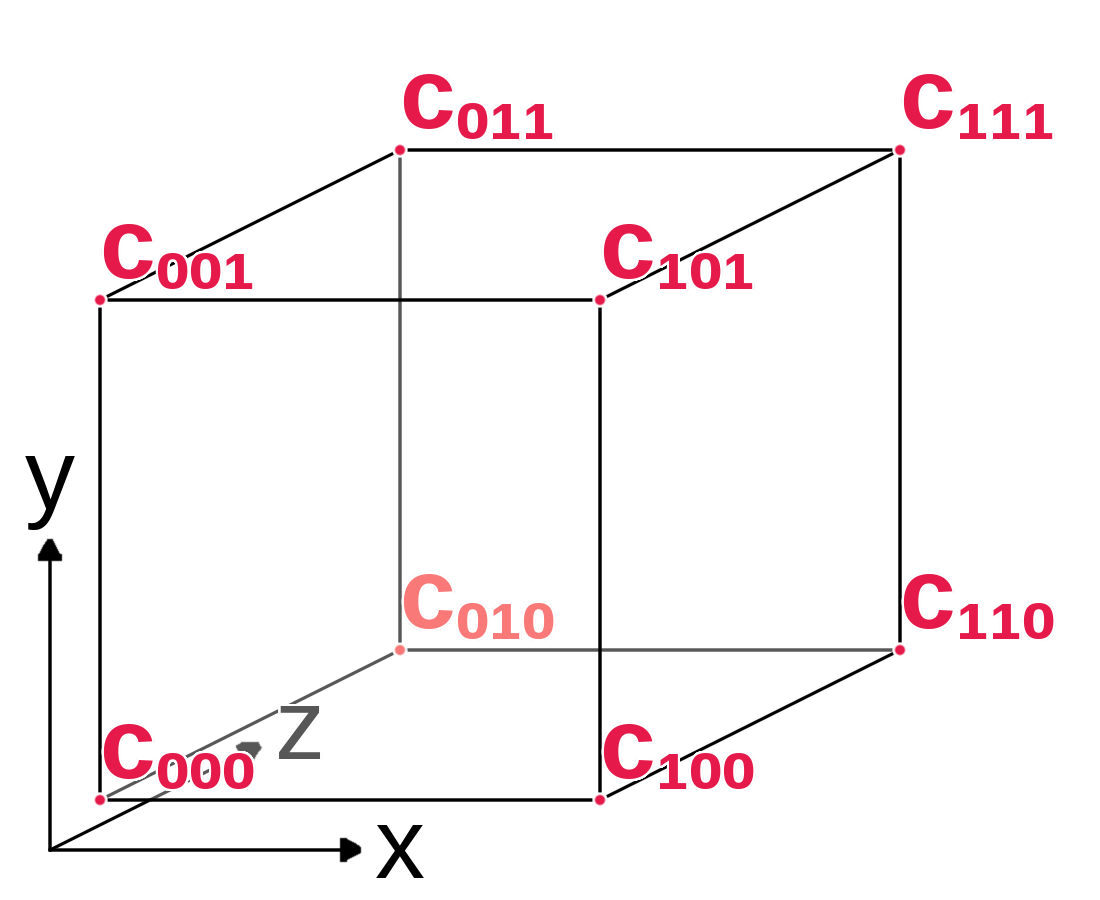
\includegraphics[width=1\textwidth]{bfield/trilinear_interpolation}
        \caption{\label{fig:trilinear_interpolation} Trilinear interpolation visual interpretation.}
    \end{wrapfigure}

Trilinear Interpolation~\cite{bourke1999interpolation} is a method that can be used to compute the value in a tridimensional space given that a regular grid of $(x,y,z)$ points and the value of the function to be interpolated $f$ is known for this set of points.

Given a point $(x,y,z)$ from which the value $f(x,y,z)$ is to be estimated, it is easy to see that the value lies inside a cube in the given regular grid with borders $(x_0, x_1)$, $(y_0, y_1)$, $(z_0, z_1)$, so that the values $c_{000}$, $c_{001}$, $c_{010}$, $c_{011}$, $c_{100}$, $c_{101}$, $c_{110}$, $c_{111}$, defined as $c_{000} = f(x_0, y_0, z_0)$, $c_{001} = f(x_0, y_0, z_1)$ and so on are already known, as seen in Figure \ref{fig:trilinear_interpolation}.

From this data, the values $x_d$, $y_d$ and $z_d$ can be obtained as:
    \begin{equation*}
        x_d = \frac{x - x_0}{x_1 - x_0},~ y_d = \frac{y - y_0}{y_1 - y_0},~ z_d = \frac{z - z_0}{z_1 - z_0}\,,
    \end{equation*}
from which linear interpolation can be done ``in steps'', first for $x$:
    \begin{align*}
        c_{00} = c_{000}(1 - x_d) + c_{100}x_d\\
        c_{01} = c_{001}(1 - x_d) + c_{101}x_d\\
        c_{00} = c_{010}(1 - x_d) + c_{110}x_d\\
        c_{00} = c_{011}(1 - x_d) + c_{111}x_d\,,
    \end{align*}
then for $y$:
    \begin{align*}
        c_0 = c_{00}(1 - y_d) + c_{10}y_d\\
        c_1 = c_{01}(1 - y_d) + c_{11}y_d\\\,,
    \end{align*}
and finally for $z$:
    \begin{equation*}
        c = c_0(1 - z_d) + c_1z_d\,,
    \end{equation*}
with $c$ denoting the interpolated $\tilde{f}(x,y,z)$ value.
\newpage
% \subsection{Multithreaded Algorithms} \label{add: multithreading}
\subsection{Fourth Order Adams-Bashforth-Moulton Method} \label{add:abm4}
The Fourth Order Adams-Bashforth-Moulton method or simply Adams-Bashforth-Moulton 4 (ABM4) is a multi-step method used to solve initial value problems similar to RK4 in use.
Solving the same equation as RK4, let an initial value problem for estimating $\mathbf{x}(z+h)$ be:

    \begin{equation*}
        \mathbf{\dot{x}} = \mathbf{f}(z,\mathbf{x}), \mathbf{x}(z_0) = \mathbf{x}_0\,,
    \end{equation*}

where the definitions are equivalent to the ones given in Section \ref{ssec:framework_rk4}.
To solve the problem using a step size $h$, first the fourth order Adams-Bashforth (AB4) method is proposed:
    \begin{equation}
        \label{eq:abm4_explicit} \mathbf{x}_{n+1}^* = \mathbf{x}_n + \frac{h}{24} (55\cdot \mathbf{f}(z, \mathbf{x}_n) - 59\cdot \mathbf{f}(z-h, \mathbf{x}_{n-1}) + 37\cdot \mathbf{f}(z-2h, \mathbf{x}_{n-2}) - 9\cdot \mathbf{f}(z-3h, \mathbf{x}_{n-3}))\,,
    \end{equation}
which is commonly denoted as the ``explicit'' AB4 method.
Then, from this result it's possible to compute a more accurate result for $\mathbf{x}_{n+1}$ using the fourth order Adams-Moulton (AM4) method, or the ``implicit'' AM4 method:
    \begin{equation}
        \label{eq:abm4_implicit} \mathbf{x}_{n+1} = \mathbf{x}_n + \frac{h}{24} (9\cdot \mathbf{f}(z+h, \mathbf{x}_{n+1}^*) + 19\mathbf{f}(z,\mathbf{x}_n) - 5\mathbf{f}(z-h,\mathbf{x}_{n-1}) + \mathbf{f}(z-2h,\mathbf{x}_{n-2})\,.
    \end{equation}
While the results of this method are not necessarily more accurate than the ones obtained by RK4 since both methods have the same convergence order, % Note: This could use a reference or an addendum explaining convergence order.
the method has the advantage that it only requires to compute $\mathbf{f}(\cdot,\cdot)$ twice for every time-step (assuming that the previous results are stored), whereas RK4 requires this function to be computed four times per time-step.
This can result in a serious improvement if the time it takes to compute $\mathbf{f}(\cdot,\cdot)$ is large.

One problem that arises from the implementation though is that at the beginning of the computation only $\mathbf{x}_0$ is known, and four steps are needed to start.
To solve this, it's not uncommon to use RK4 to compute $\mathbf{x}_1$, $\mathbf{x}_2$ and $\mathbf{x}_3$ and then start using ABM4.
% \subsection{Colorblind-Friendly Palette} \label{add:colorblind_palette}
\subsection{Code and Reproducibility} \label{add:code_and_reproducibility}
The original CLAS12-offline-software repository can be found in:

\texttt{https://github.com/JeffersonLab/clas12-offline-software}

while the commit it was in as the project started is \texttt{fb6d5b2} (link last accessed as of September $27$ $2019$).

\newpage

The repository's fork where the author's work can be found in is:

\texttt{https://github.com/bleaktwig/clas12-offline-software}

and the commit by the end of this project's development is \texttt{12924ec} (link last accessed as of September $27$ $2019$).

The contact information for the people behind the software, CLAS12 and Hall B is as follows:

    \begin{itemize}
        \item V. Ziegler, CLAS12 Software Project Coordinator (\texttt{ziegler@jlab.org}) 757-269-6003
        
        \item L. Elouadrhiri, Control Account Manager (\texttt{latifa@jlab.org}) 757-269-7303
        
        \item G. Young, Associate Project Manager for Physics (\texttt{young@jlab.org}) 757-269-6904
        
        \item V. D. Burkert, Hall B Group Leader (\texttt{burkert@jlab.org}) 757-269-7540
    \end{itemize}


    \newpage

    \bibliographystyle{apalike}
    \bibliography{21references}{}
\end{document}

% Note: The chapter references are hardcoded due to a bug in the format. If for any reason the chapters change order, figure out where the references are by searching for "CHAPTER REFERENCE".